%!TEX root = ../main.tex
\chapter{Timing study of hadron showers}
\label{chap:TimingPions}

In this chapter, the recorded pion data is compared to \geant v10.1 simulations using different hadronic models as explained in chapter \ref{chap:G4Simulation}.

\section{Dataset}

The pion dataset used in this study is selected based on criteria described in section \ref{sec:pionsel}. The same time calibration constants and corrections determined from muons and electrons is applied to the pion data. The table \ref{table:pion_runs} summarizes the runs and datasets used for the pion analysis. N$_{3 T_0}$ is the number of events after the selection on the time reference (see section \ref{section:time_ref}). N$_{sel.}$ is the number of events after the cut on the error of the time reference.

\begin{table}[htb!]
	\centering
	\caption{Table with the number of events selected in the pion dataset for the timing study.}
	\label{table:pion_runs}
	\begin{tabular}{@{} llllll @{}}
		\toprule
		Runs & Energy & Particle Type & N$_{3 T_0}$ & N$_{sel.}$ & $\frac{\text{N$_{sel.}$}}{\text{N$_{3 T_0}$}}$ \\
		\midrule
		\makecell{24306-24317 \\ 24381-24397} & 10 GeV & $\pi^-$ & 425517 & 349012 & 82\% \\
		\midrule
		24578-24612 & 50 GeV & $\pi^-$ & 1183790 & 1007889 & 85.1\% \\
		24339-24342 & 70 GeV & $\pi^-$ & 142813 & 122376 & 85.7\% \\
		\midrule
		\makecell{24223-24238 \\ 24273-24287\\ 24331-24336\\ 24358-24364} & 90 GeV & $\pi^-$ & 466927 & 395884 & 84.8\% \\
		\bottomrule
	\end{tabular}
\end{table}

\section{Time of first hit distribution}

Inside a hadronic shower, absorber materials with a high atomic number Z, thus containing a high number of neutrons, are expected to release a high number of evaporation neutrons. These neutrons then will deposit energy by two different mechanisms with different time scales relative to the first hard interaction.

First, the elastic scattering of neutrons in the active material especially with high hydrogen content will play a role at a few nanoseconds to tens of nanoseconds time scale, whereas neutron capture in the absorber material at the interface with the active material will contribute to several hundred or thousands of nanoseconds timescale due to the relatively long time of flight of thermal neutrons and the lifetime of such atomic states. Thus it is expected that hadronic showers will present an increase in the late component, i.e an increase in the right tail of the time distribution, compared to muons or electrons time distributions.

\begin{figure}[htbp!]
	\centering
	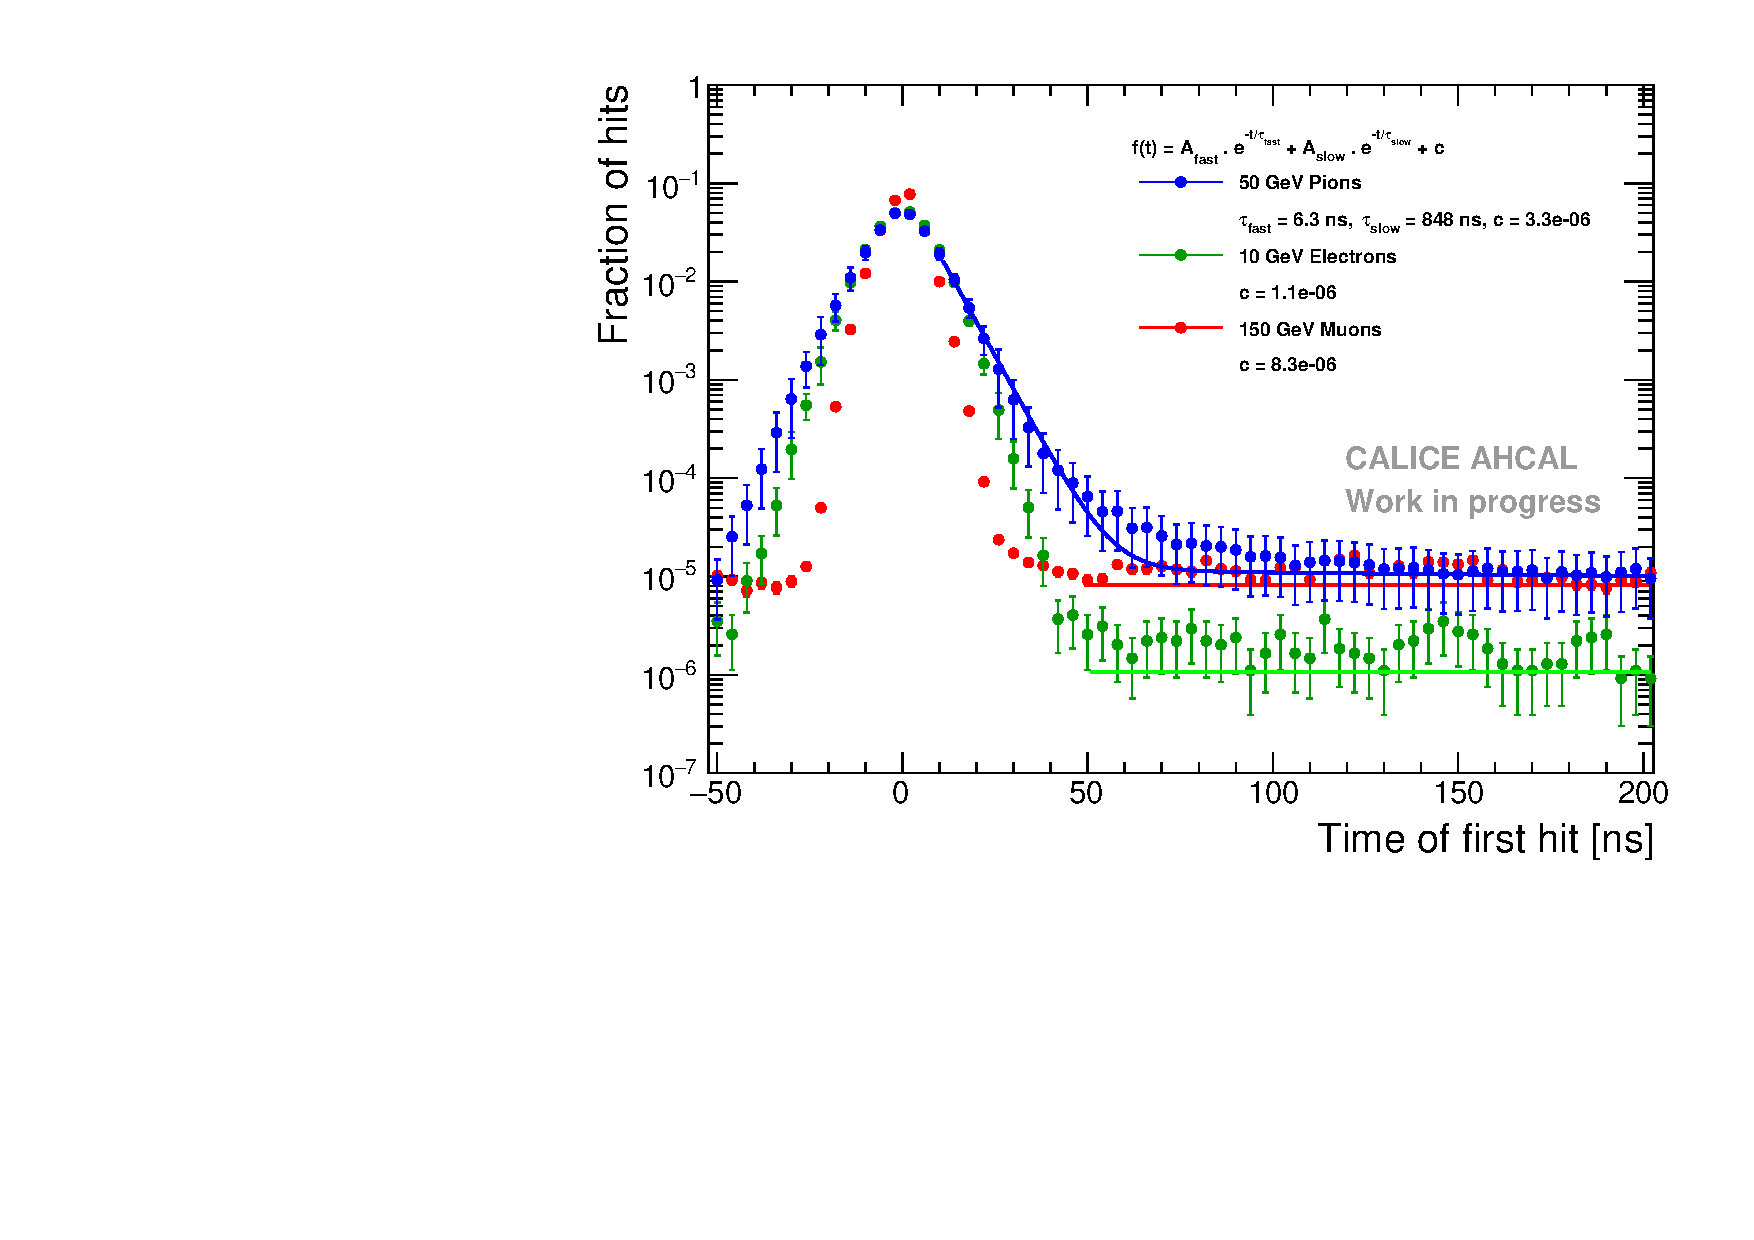
\includegraphics[width=0.6\textwidth]{../Thesis_Plots/Timing/Pions/Plots/Timing_dNdt_Comparison.pdf}
	\caption{Time of first hit for muons, electrons and pions in steel absorber in a range of -50 to 200 ns. The histograms are normalized to the number of events. The lines represent the fit to the data as explained in the text.}
	\label{fig:dNdt_Comparison}
\end{figure}

Figure \ref{fig:dNdt_Comparison} shows the time of first hit for muons, 10 GeV electrons and 50 GeV pions. Energy depositions from muons and electrons are instantaneous within a certain time window centered around 0 ns that is determined by the intrinsic time resolution of the detector. Some isolated hits are present in the tails most likely caused by SiPM thermal noise. This gives an idea of the noise level as well as the rejection of noise in the analysis. One can remark that the noise level in electron data is lower than in the muon data. The reason is not clear. It may come from the difference in beam rate and differences in the detector threshold configurations for different beams. For muons, around 2\% of hits are later than 50 ns compared to the core of the distribution between -50 and 50 ns. For electrons, 0.37\% of hits are later than 50 ns. For pions, about 1.5\% of hits are after 50 ns. However, the noise level is similar on both sides of the time distribution for muons and electrons giving confidence that the tails are coming from noise hits and not physics.

The pion time distribution presents a higher tail between 30 to 50 ns than the electron time distribution. In order to characterize the distribution, a model of the sum of two exponentials and a constant, similar as the T3B experiment \cite{Simon2013} is applied following the equation \ref{eq:dNdt_eq}:

\begin{equation} \label{eq:dNdt_eq}
	\frac{1}{N}\frac{dN}{dt} = A_{fast} \times e^{-\frac{t}{\tau_{fast}}} + A_{slow} \times e^{-\frac{t}{\tau_{slow}}} + c
\end{equation}

where $A_{fast}, \tau_{fast}$ and $A_{slow}, \tau_{slow}$ are the amplitudes and decays times of the modeled fast and slow component of the hadronic shower. Since the fit is performed on several orders of magnitudes, the same fitting method that the T3B experiment uses is applied. It is done in two steps. First, the slow component and the constant are fitted between 90 ns and \SI{2}{\micro\second}. Then, the parameters of the slow component and the constant are fixed and then the fast component is fitted between 10 ns to \SI{2}{\micro\second}.

With this procedure, a fast component of $6.03 \pm 0.41$ ns and a slow component of $848 \pm 365$ ns are fitted. The time constant of the fast component is in the same order of magnitude as given by T3B of 8 ns and is interpreted by the evaporation neutrons energy depositions in the active medium. But due to the time resolution of the AHCAL being in the same order of magnitude, it is difficult to confirm this origin.

However, the time constant of the slow component is very different than in the T3B experiment (around 80 ns in steel). This may be due to the contribution of SiPM noise which is in the order of \SI{1}{\micro\second}. It reduces the sensitivity to this slow component in the shower. One can remark that this model may be incomplete as the fitting function does match well the data in the transition region of 50 to 100 ns. This is similarly observed in the T3B data. The table \ref{table:dNdt_fit} sums up the fitted results.

\begin{table}[htb!]
	\centering
	\caption{Summary of the fit results in figure \ref{fig:dNdt_Comparison}.}
	\label{table:dNdt_fit}
	\begin{tabular}{@{} lccc @{}}
		\toprule
		Parameter & Muon & Electron & Pion \\
		\midrule
		$\tau_{fast}$ [ns] & - & - & $6.03 \pm 0.41$ \\
		$\tau_{slow}$ [ns] & - & - & $848 \pm 365$ \\
		$c$ & $(8.27 \pm 0.05) \times 10^{-6}$ & $(1.06 \pm 0.03) \times 10^{-6}$ & $(3.25 \pm 1.08) \times 10^{-6}$ \\
		\bottomrule
	\end{tabular}
\end{table}

Figure \ref{fig:dNdt_SimData_10GeV} shows the time distribution of first hits compared with three different physics lists for 10 GeV pions. Additional distribution for higher pion beam energies are shown in appendix \ref{appendix:TimingAdd}. For the core of the distribution under 50 ns, overall, all physics lists describe relatively well the data within the systematics.

From 10 to 50 GeV, the QGSP\_BERT\_HP physics list reproduces well the distribution. Above 50 GeV, the tail after 100 ns is also well described in the simulation, however, between 50 and 100 ns, the simulation slightly under-estimates the data although within the systematic uncertainty.

The QBBC physics list tends to over-estimate the late tail by around a factor 2. This does not agree with the observations made in the T3B experiment where the QBBC physics list agrees well with the time distribution for 60 GeV pions. It may be related to the use of different \geant versions because the T3B experiment has used \geant v9.4p03.

For all time of first hit distributions, the QGSP\_BERT physics list over-estimates the tail of the distribution by around a factor 10.

\begin{figure}[htbp!]
	\begin{subfigure}[t]{0.49\textwidth}
		\centering
		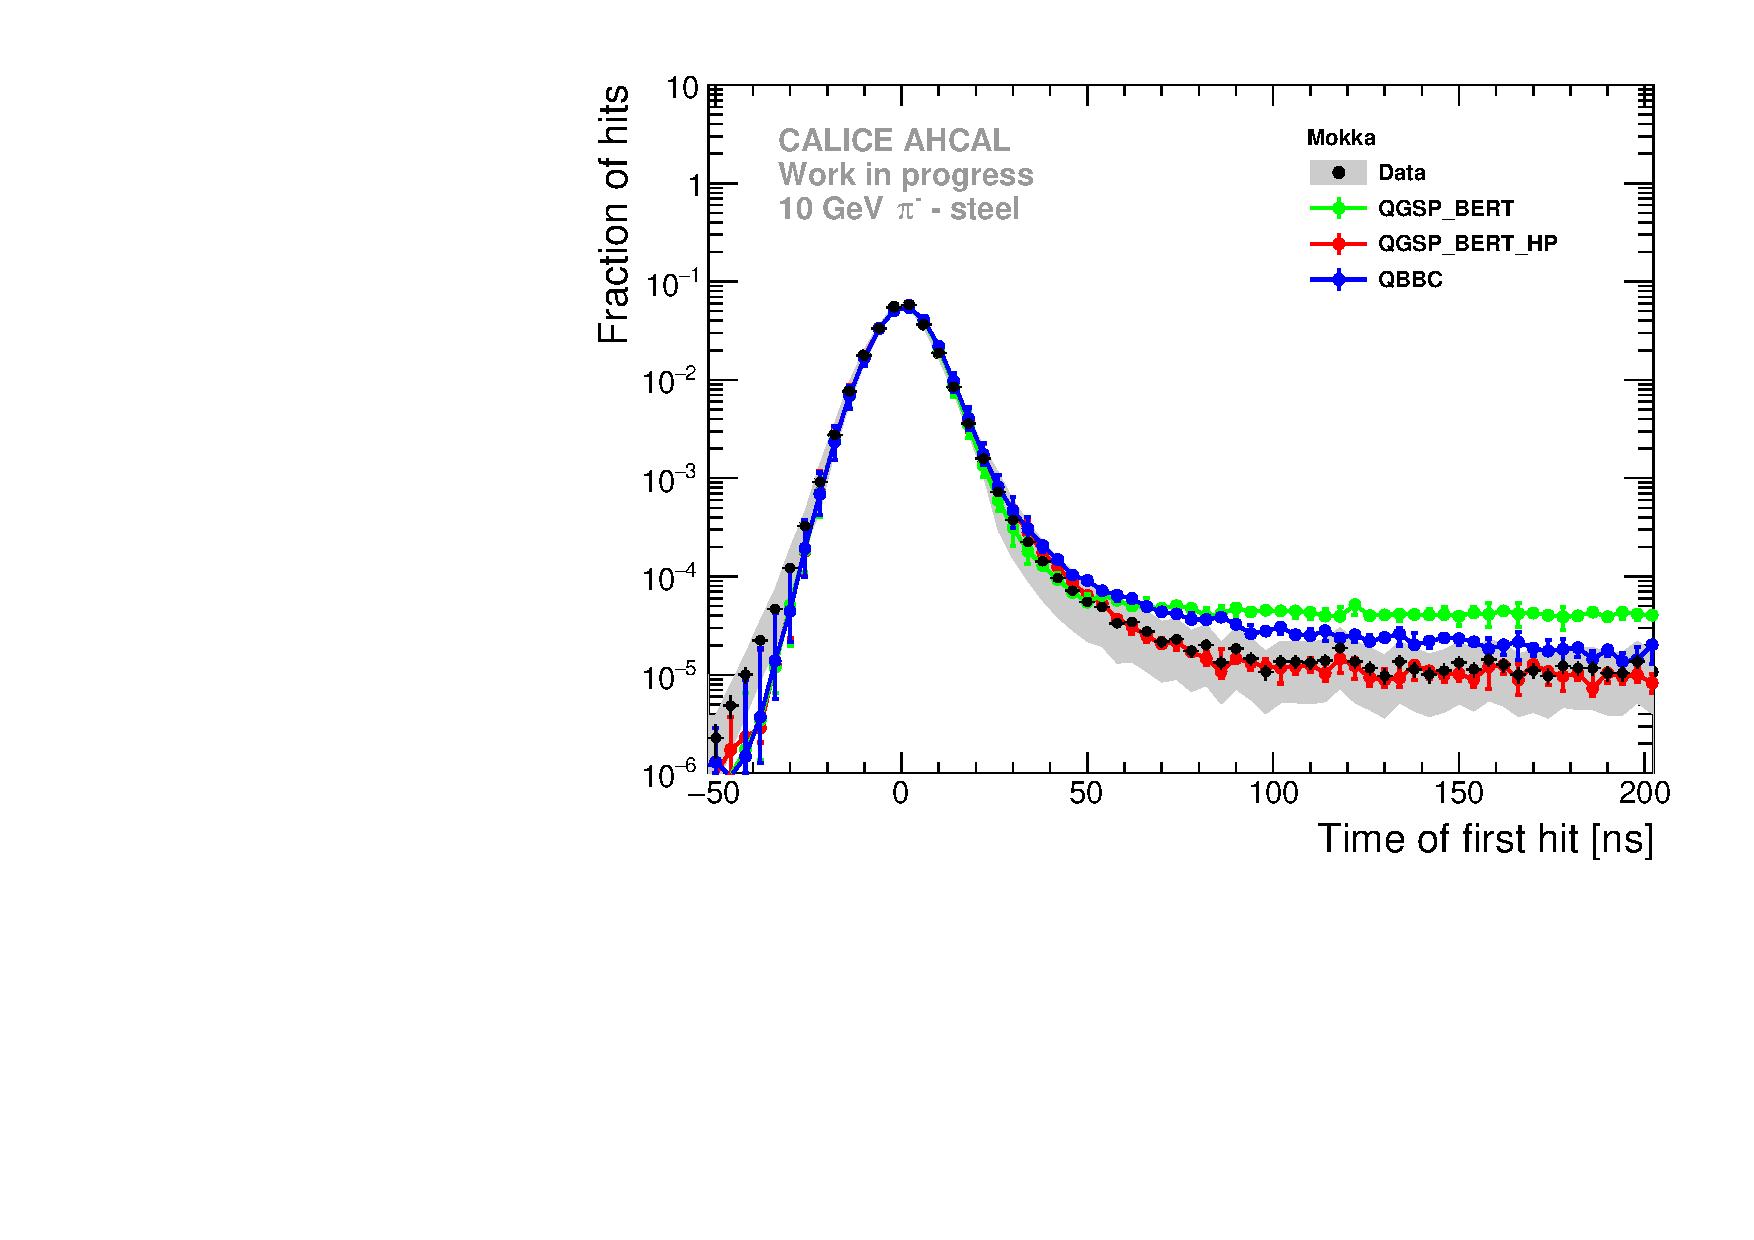
\includegraphics[width=1\textwidth]{../Thesis_Plots/Timing/Pions/Plots/Comparison_SimData_Pion10GeV_LateClusters.pdf}
		\caption{}
	\end{subfigure}
	\hfill
	\begin{subfigure}[t]{0.49\textwidth}
		\centering
		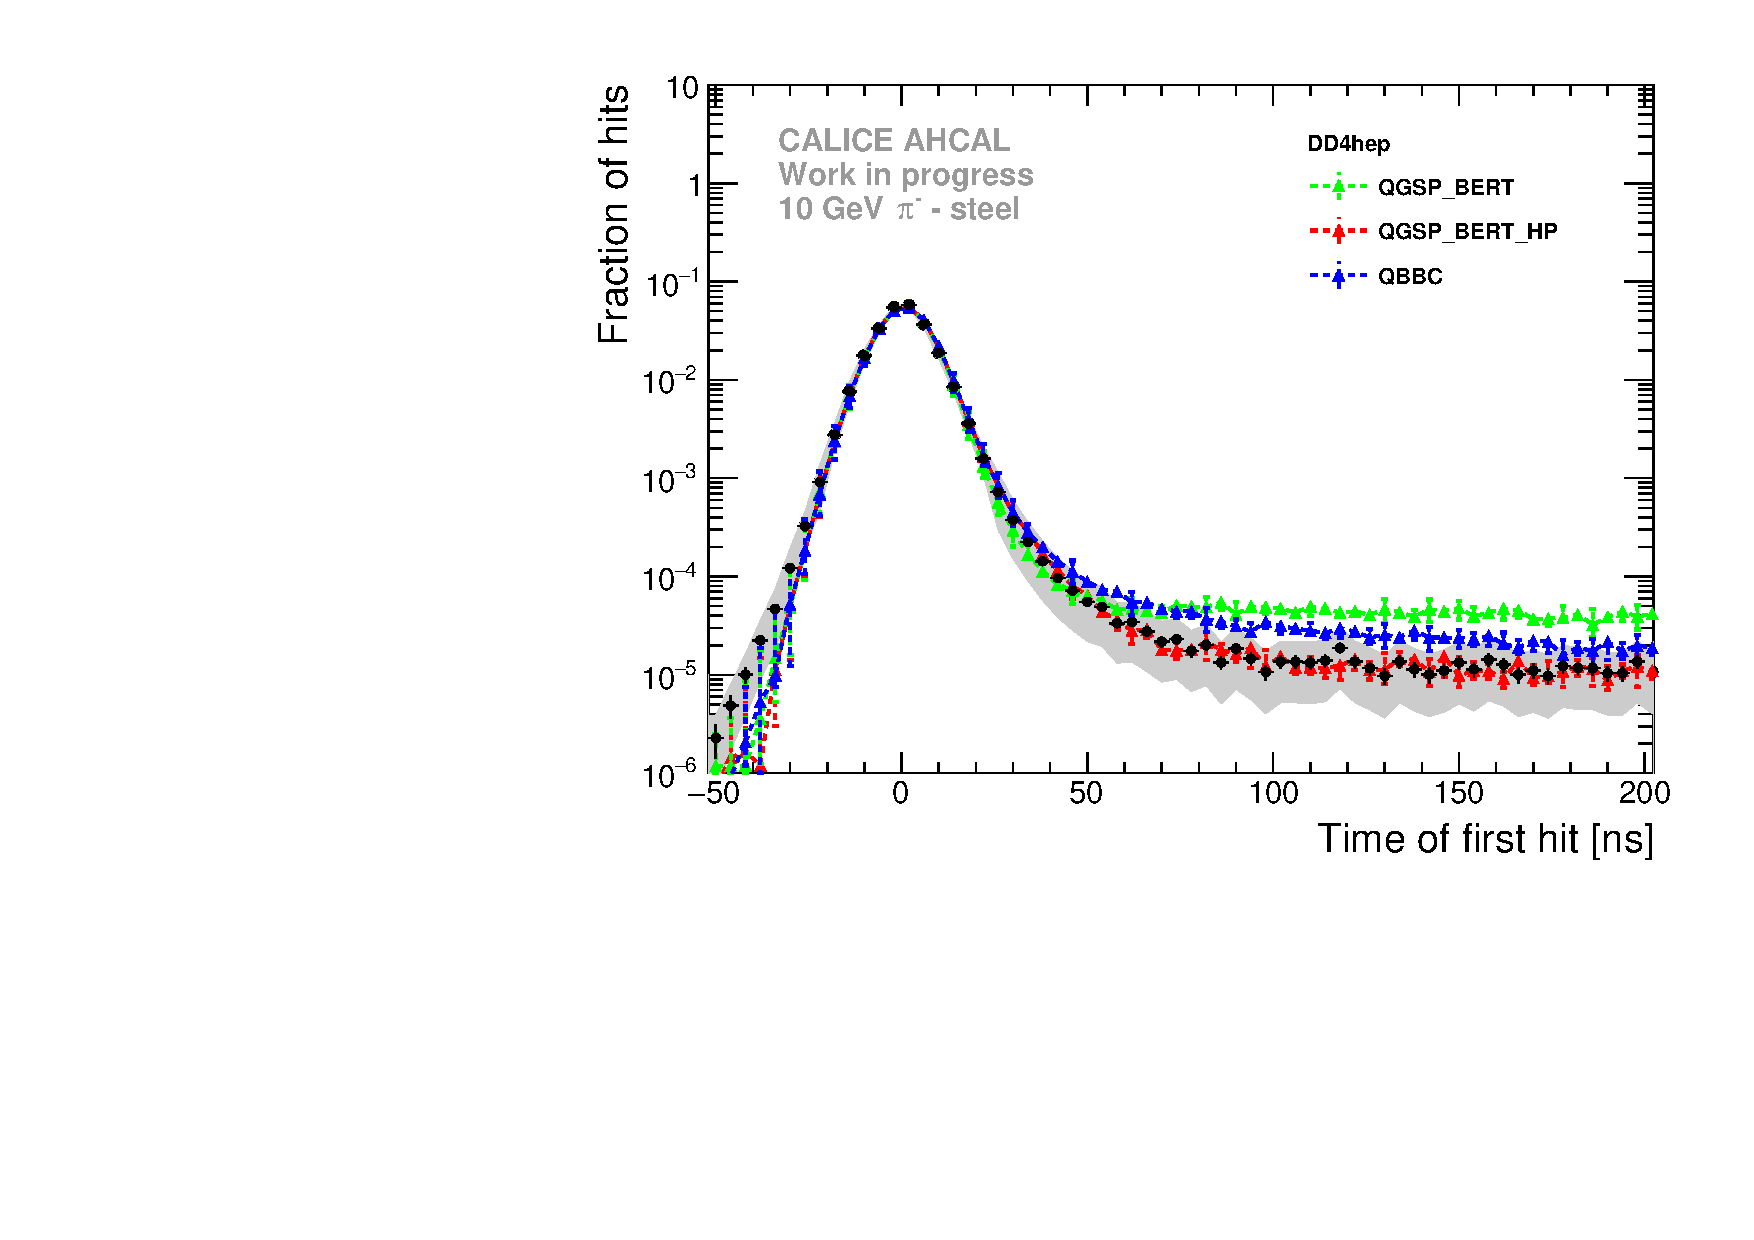
\includegraphics[width=1\textwidth]{../Thesis_Plots/Timing/Pions/Plots/Comparison_SimData_Pion10GeV_LateClusters_DD4hep.pdf}
		\caption{}
	\end{subfigure}
	\caption{Comparison of the time of first hit distribution for 10 GeV pions in data and three different physics list for \mokka (left) and \ddhep (right) simulations. The grey and color bands shows the statistical and systematic uncertainties.} 	\label{fig:dNdt_SimData_10GeV}
\end{figure}

\section{Energy dependence of the time of first hit}

The dependence in energy of the time of first hit has been studied in the following. It is expected that there is no energy dependence for muon and electron beams as these are quasi-instantaneous. On the other hand, for pions, it is expected that low energy hits mostly coming from neutron signals in the calorimeter are delayed.

The mean time of the first hit taken in a time window of -50 ns to 200 ns as a function of the hit energy is shown in figure \ref{fig:Energy_Comparison} for muon, electron and pion beams. For muons and electrons, no dependence on energy is observed as expected, all hits are instantaneous independent of their energy. For 10 GeV pions, a delay of 2-3 ns at 0.5 MIP is observed and decreases down to 0-1 ns above 1 MIP. For higher pion energies, the mean time of the first hit decreases between 0.5 and 1.5 MIP then increases for hit energies above 1.5 MIPs. This is not expected, thus individual distributions have been checked. An example is shown in figure \ref{fig:TimeBinsEnergy} for 90 GeV pions. After 1.5 MIP, the time distribution gets wider and the maximum of the distribution is de-centered slightly from 0 ns, therefore explaining the increase of the mean time of the first hit for hit energies over 1.5 MIP. This may be coming from an imperfect time correction as a function of the number of triggered channels in a chip (see section \ref{subsec:ped_shift}) as mostly high energy hits are coming from the electromagnetic core of the hadronic shower.

\begin{figure}[htbp!]
	\begin{subfigure}[t]{0.49\textwidth}
		\centering
		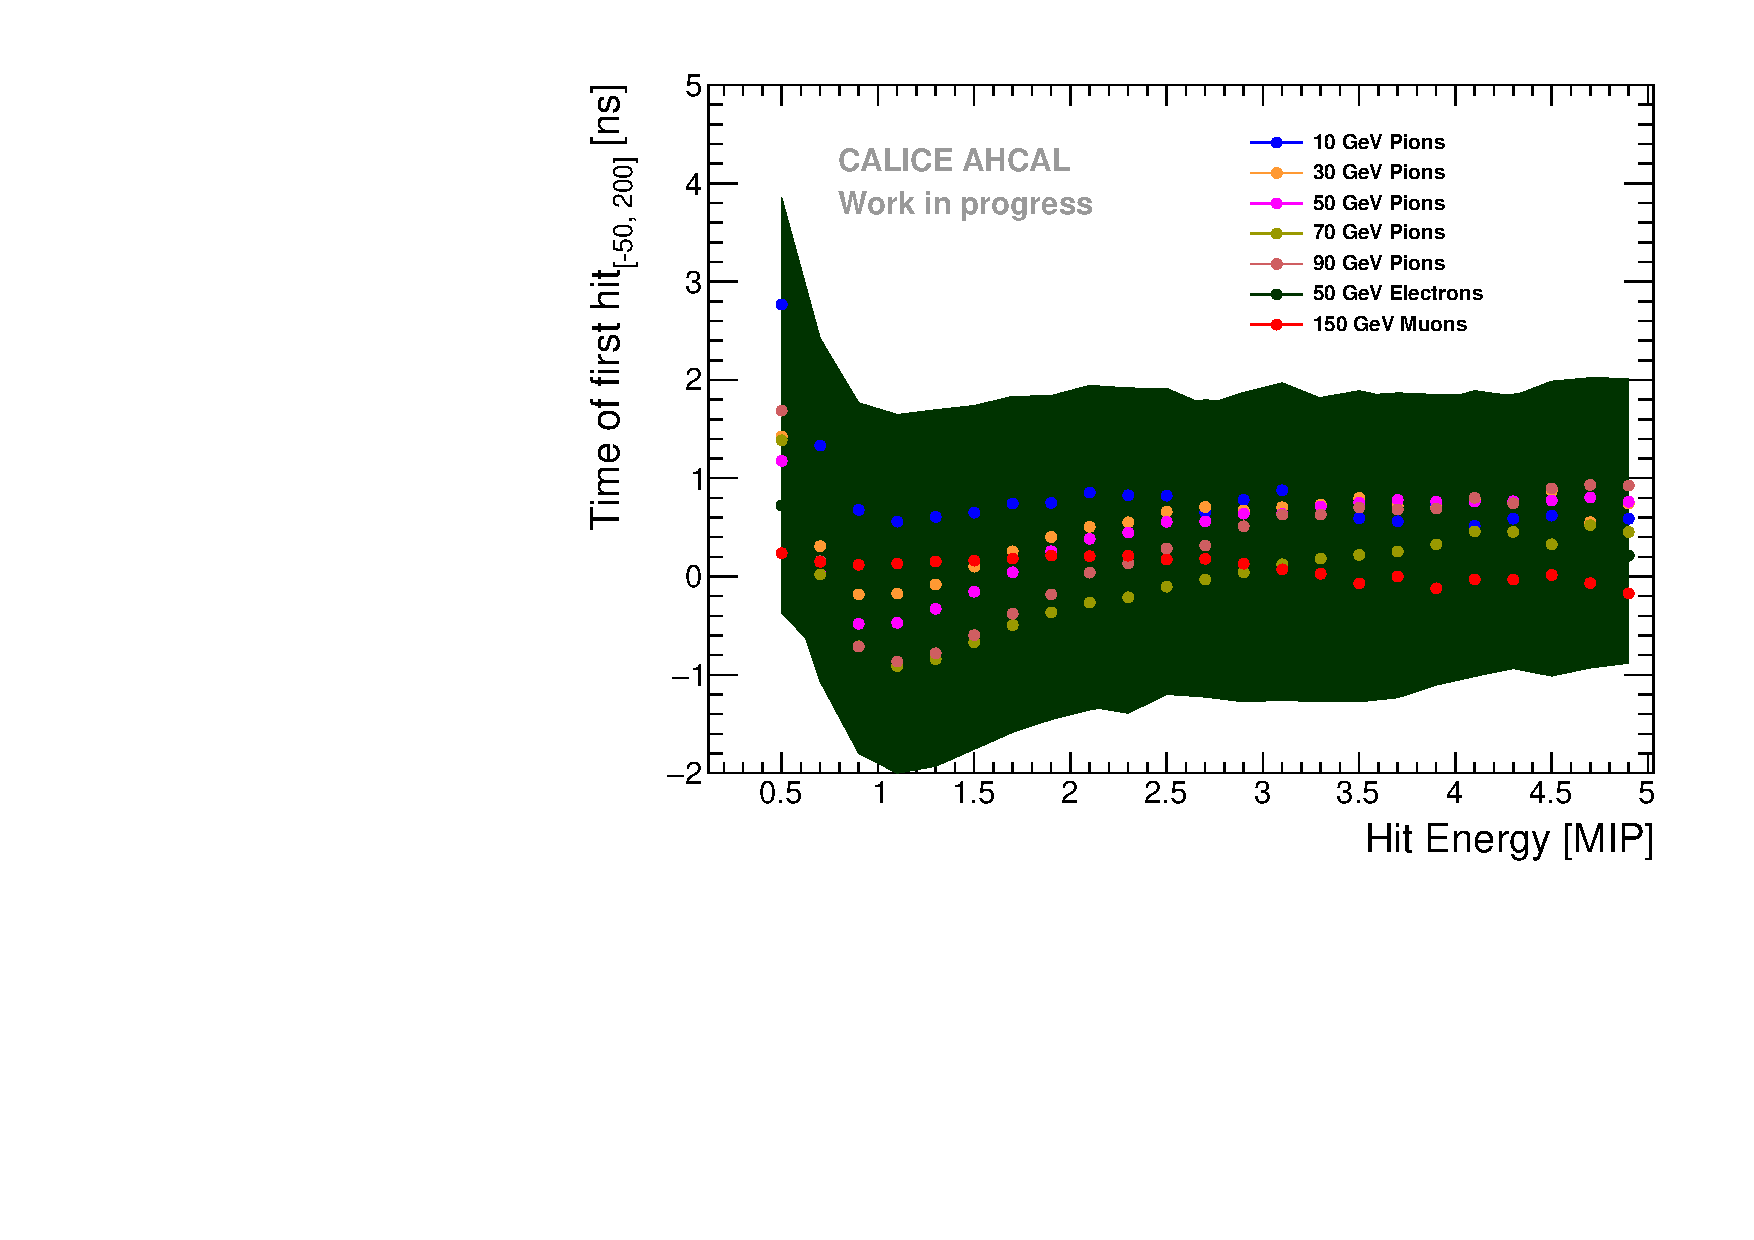
\includegraphics[width=1\textwidth]{../Thesis_Plots/Timing/Pions/Plots/Timing_Energy_Comparison_ShortAsymRange.pdf}
		\caption{} \label{fig:Energy_Comparison}
	\end{subfigure}
	\hfill
	\begin{subfigure}[t]{0.49\textwidth}
		\centering
		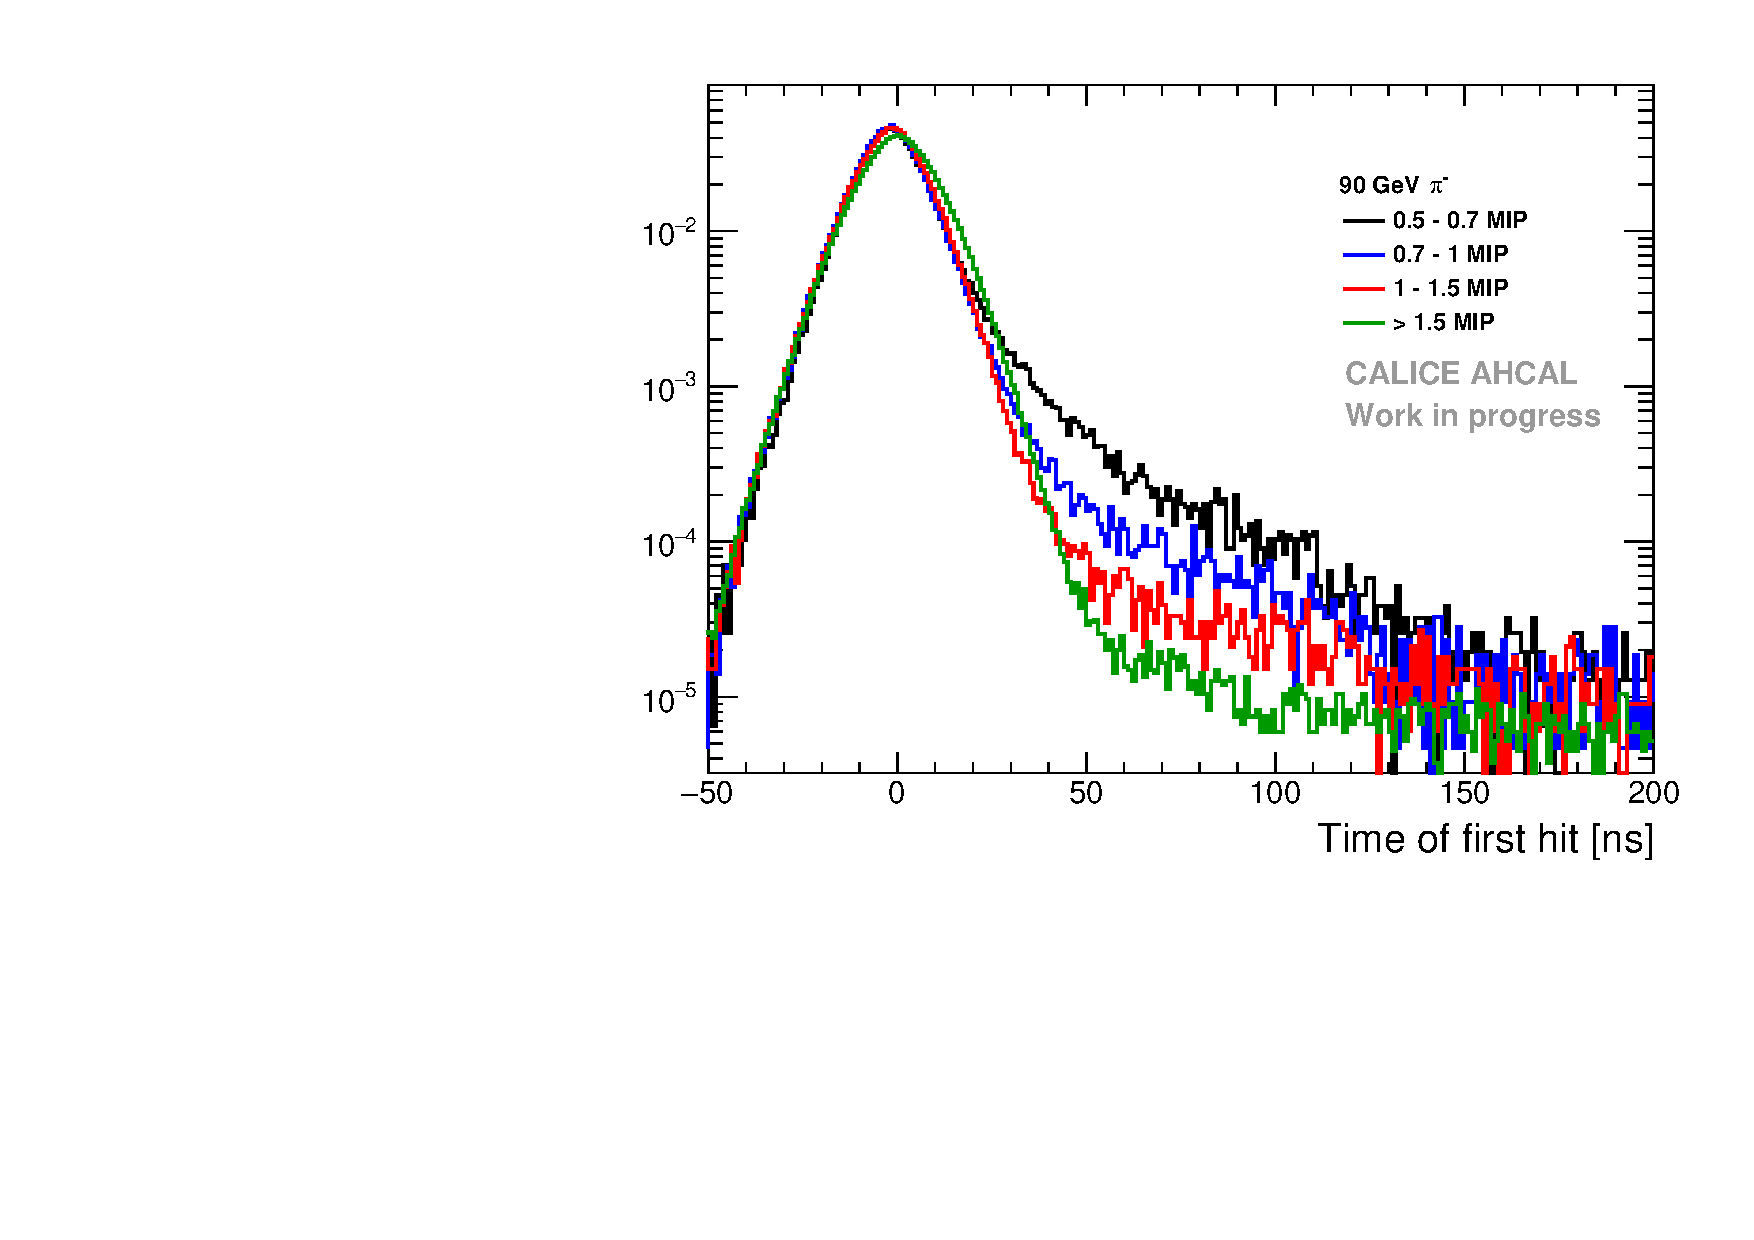
\includegraphics[width=1\textwidth]{../Thesis_Plots/Timing/Pions/Plots/TimeEnergyBinsPions.pdf}
		\caption{} \label{fig:TimeBinsEnergy}
	\end{subfigure}
	\caption{On the left, time of first hit as function of the hit energy for muons, electrons and pions in steel absorber in a range of -50 to 200 ns. The bands represent the systematic uncertainty. On the right, time distribution for 90 GeV pions for different hit energy ranges.}
\end{figure}

Figures \ref{fig:Energy_SimData_10GeV} and \ref{fig:Energy_SimData_90GeV} show the comparison of the mean time of first hit as a function of the hit energy in data and simulations for 10 GeV and 90 GeV pions. For other pion beam energies and the \ddhep simulation, the figures are available in appendix \ref{appendix:TimingAdd}. For 10 GeV pions, the simulation reproduces well the data within the systematics. For higher energies, a difference is visible in the region 0.5 to 1.5 MIP where the simulation is above the data. Above 1.5 MIPs, the data and simulations agree well. Firstly, a difference is visible between the QGSP\_BERT and QGSP\_BERT\_HP physics lists mainly between hit energies of 1-3 MIPs but, in general, the difference is smaller than the systematic uncertainty on the data. Secondly, the QGSP\_BERT and QBBC physics lists are very similar over the full hit energy range. Finally, all models show an increase of the mean time of first hit at small hit energies with higher beam energy. The data does not reflect this.

\begin{figure}[htbp!]
	\begin{subfigure}[t]{0.49\textwidth}
		\centering
		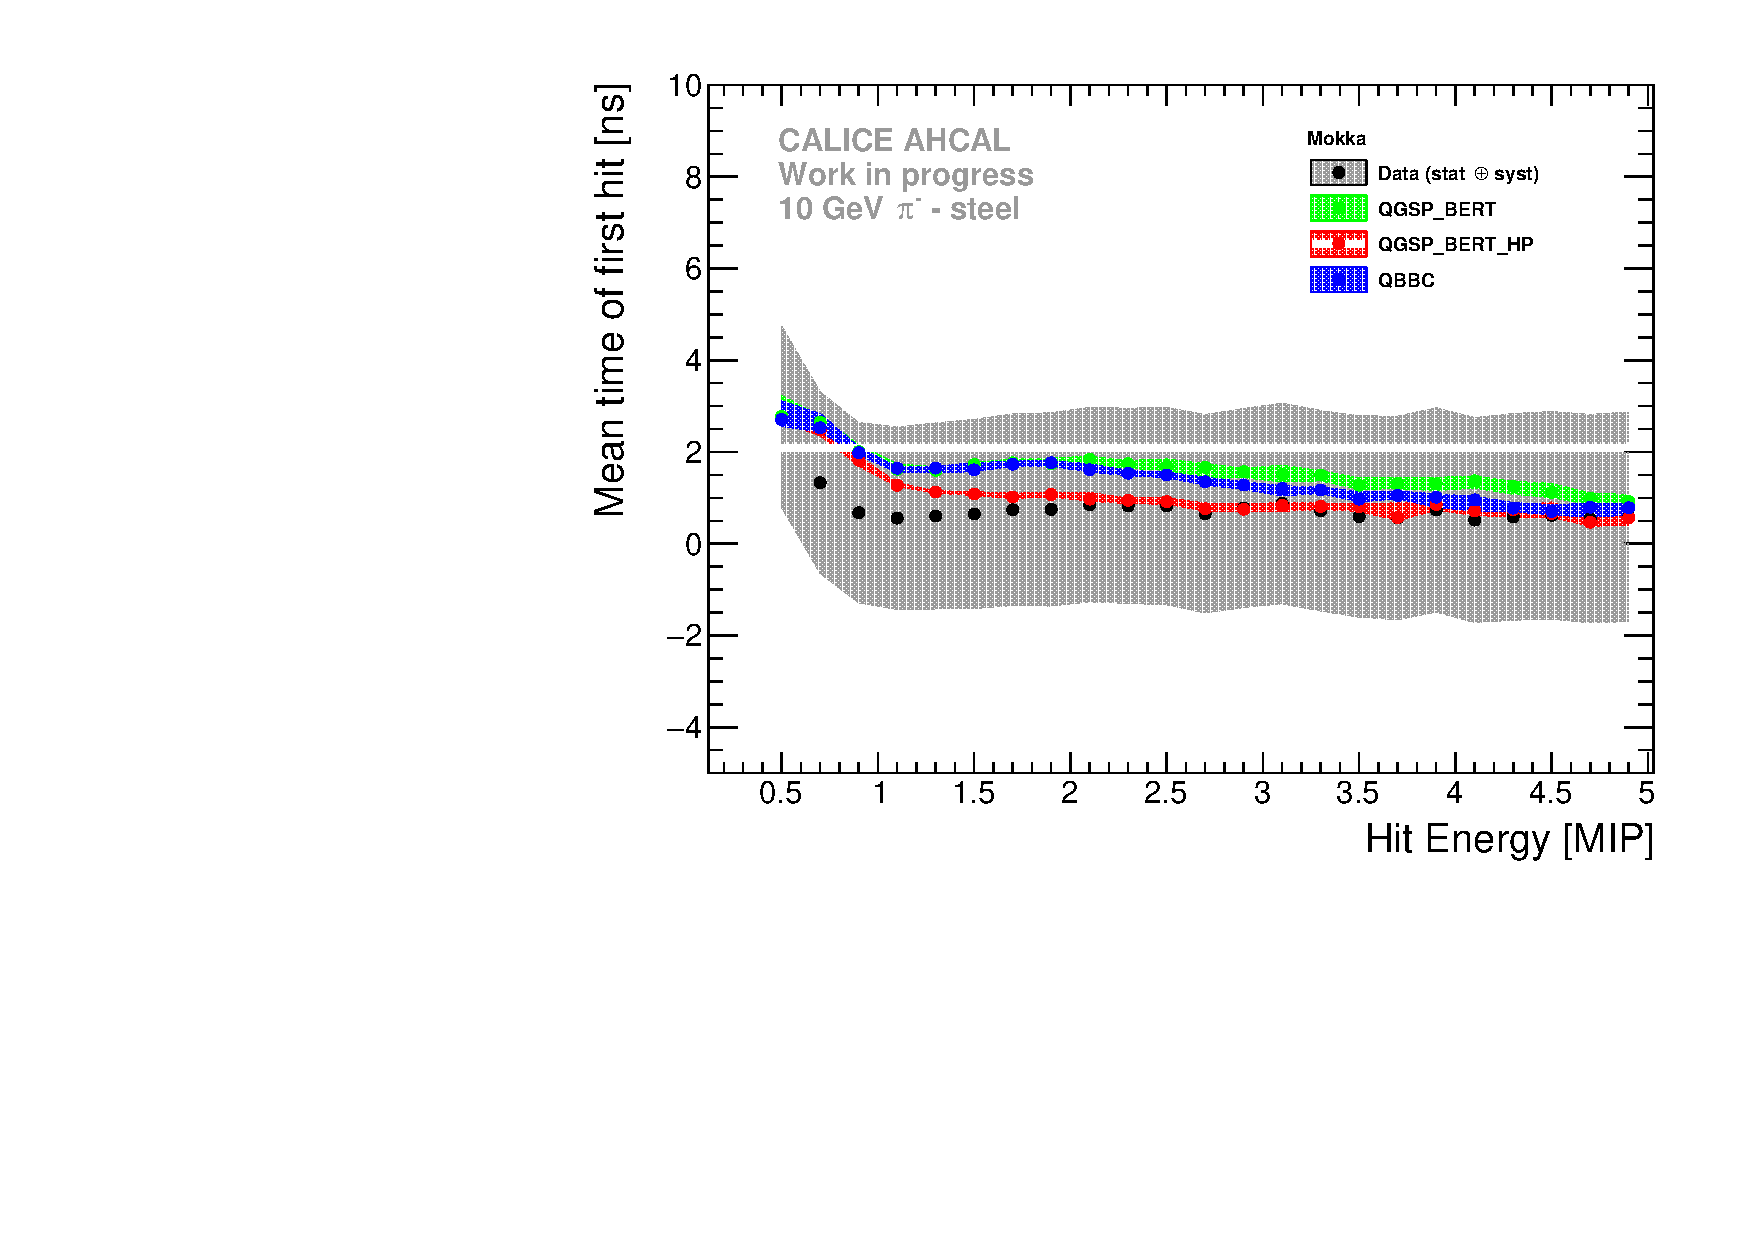
\includegraphics[width=1\textwidth]{../Thesis_Plots/Timing/Pions/Plots/ComparisonToSim/Time_Energy_10GeV_Mokka.pdf}
		\caption{} \label{fig:Energy_SimData_10GeV}
	\end{subfigure}
	\hfill
	\begin{subfigure}[t]{0.49\textwidth}
		\centering
		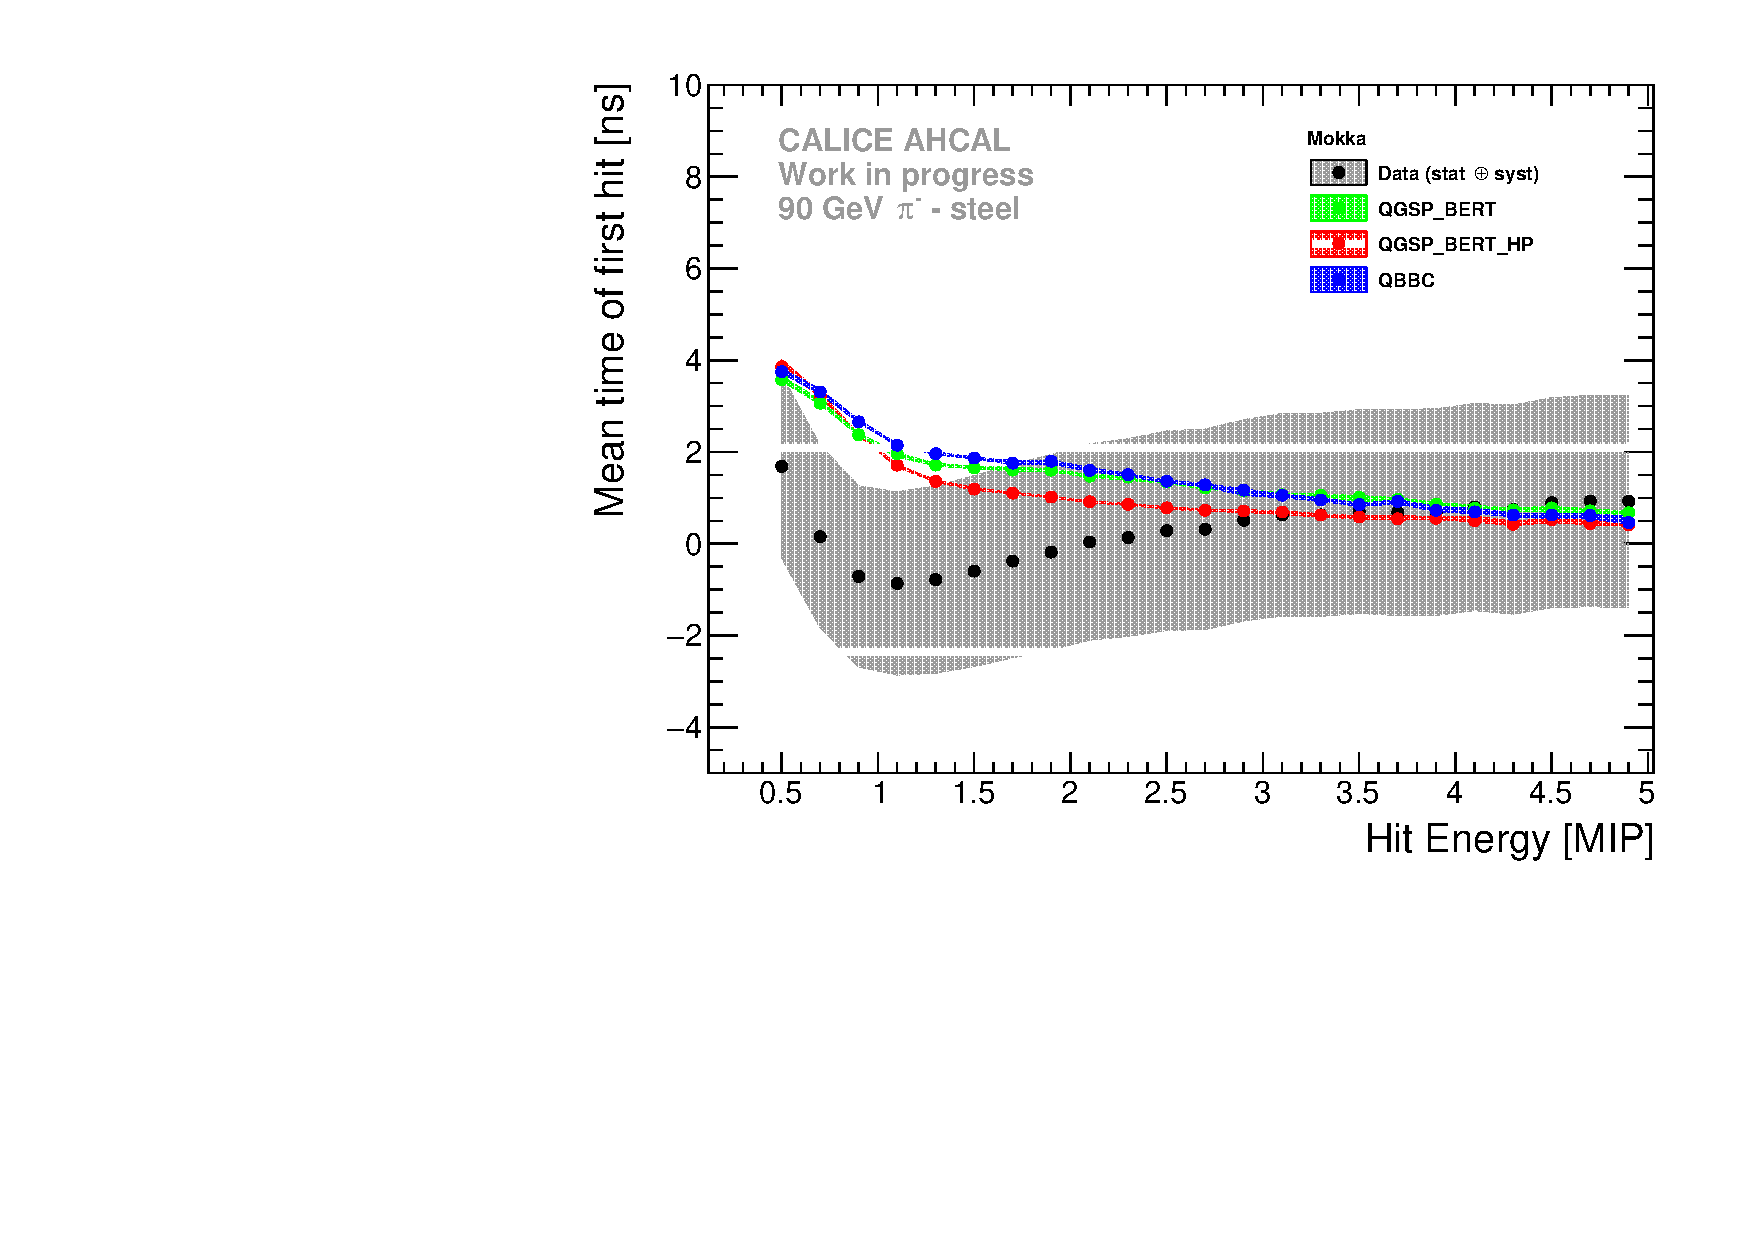
\includegraphics[width=1\textwidth]{../Thesis_Plots/Timing/Pions/Plots/ComparisonToSim/Time_Energy_90GeV_Mokka.pdf}
		\caption{} \label{fig:Energy_SimData_90GeV}
	\end{subfigure}
	\caption{Comparison of the mean time of the first hit as function of the hit energy in data and \mokka simulation for 10 GeV and 90 GeV pions. The grey and color bands shows the statistical and systematic uncertainties.}
\end{figure}

This comparison study seems to confirm that low energy hits are responsible for delayed energy depositions in the calorimeter, most likely due to low energy neutrons from capture and spallation processes. Higher energy deposits occur mostly in the prompt part of the hadron shower.

\section{Radial dependence of the time}
\label{sec:RadialTime}

The prompt component of a hadron shower is dominated by EM sub-showers and relativistic particles, whereas the delayed component is coming from mostly evaporation and spallation low energy neutrons. It is expected that the former is concentrated near the shower axis, while the latter, is spread out laterally as these neutrons can travel far away in the calorimeter before interacting.

This is investigated by looking at the mean time of first hit as a function of the hit distance to the shower center of gravity defined in the x-y plane of the calorimeter. For the muon data, the hit position in the detector relative to (0,0) is used. The mean time of the first hit as a function of the hit distance to the shower center of gravity is shown in figure \ref{fig:Radius_Comparison_SSF} for the layers 3 to 10 and in figure \ref{fig:Radius_Comparison_BL} the layers 11 to 14 separately. The layers needed to be separated because of a decrease of the mean time of first hit at the distance where there is a transition between a HBU (layers 3 to 10) and a 2 by 2 HBU (layers 11 to 14). This is thought that this effect may be related to the starting point of the pion shower. This is investigated in more details in section \ref{sec:TimeRadiusDepth}.

\begin{figure}[htbp!]
	\begin{subfigure}[t]{0.49\textwidth}
		\centering
		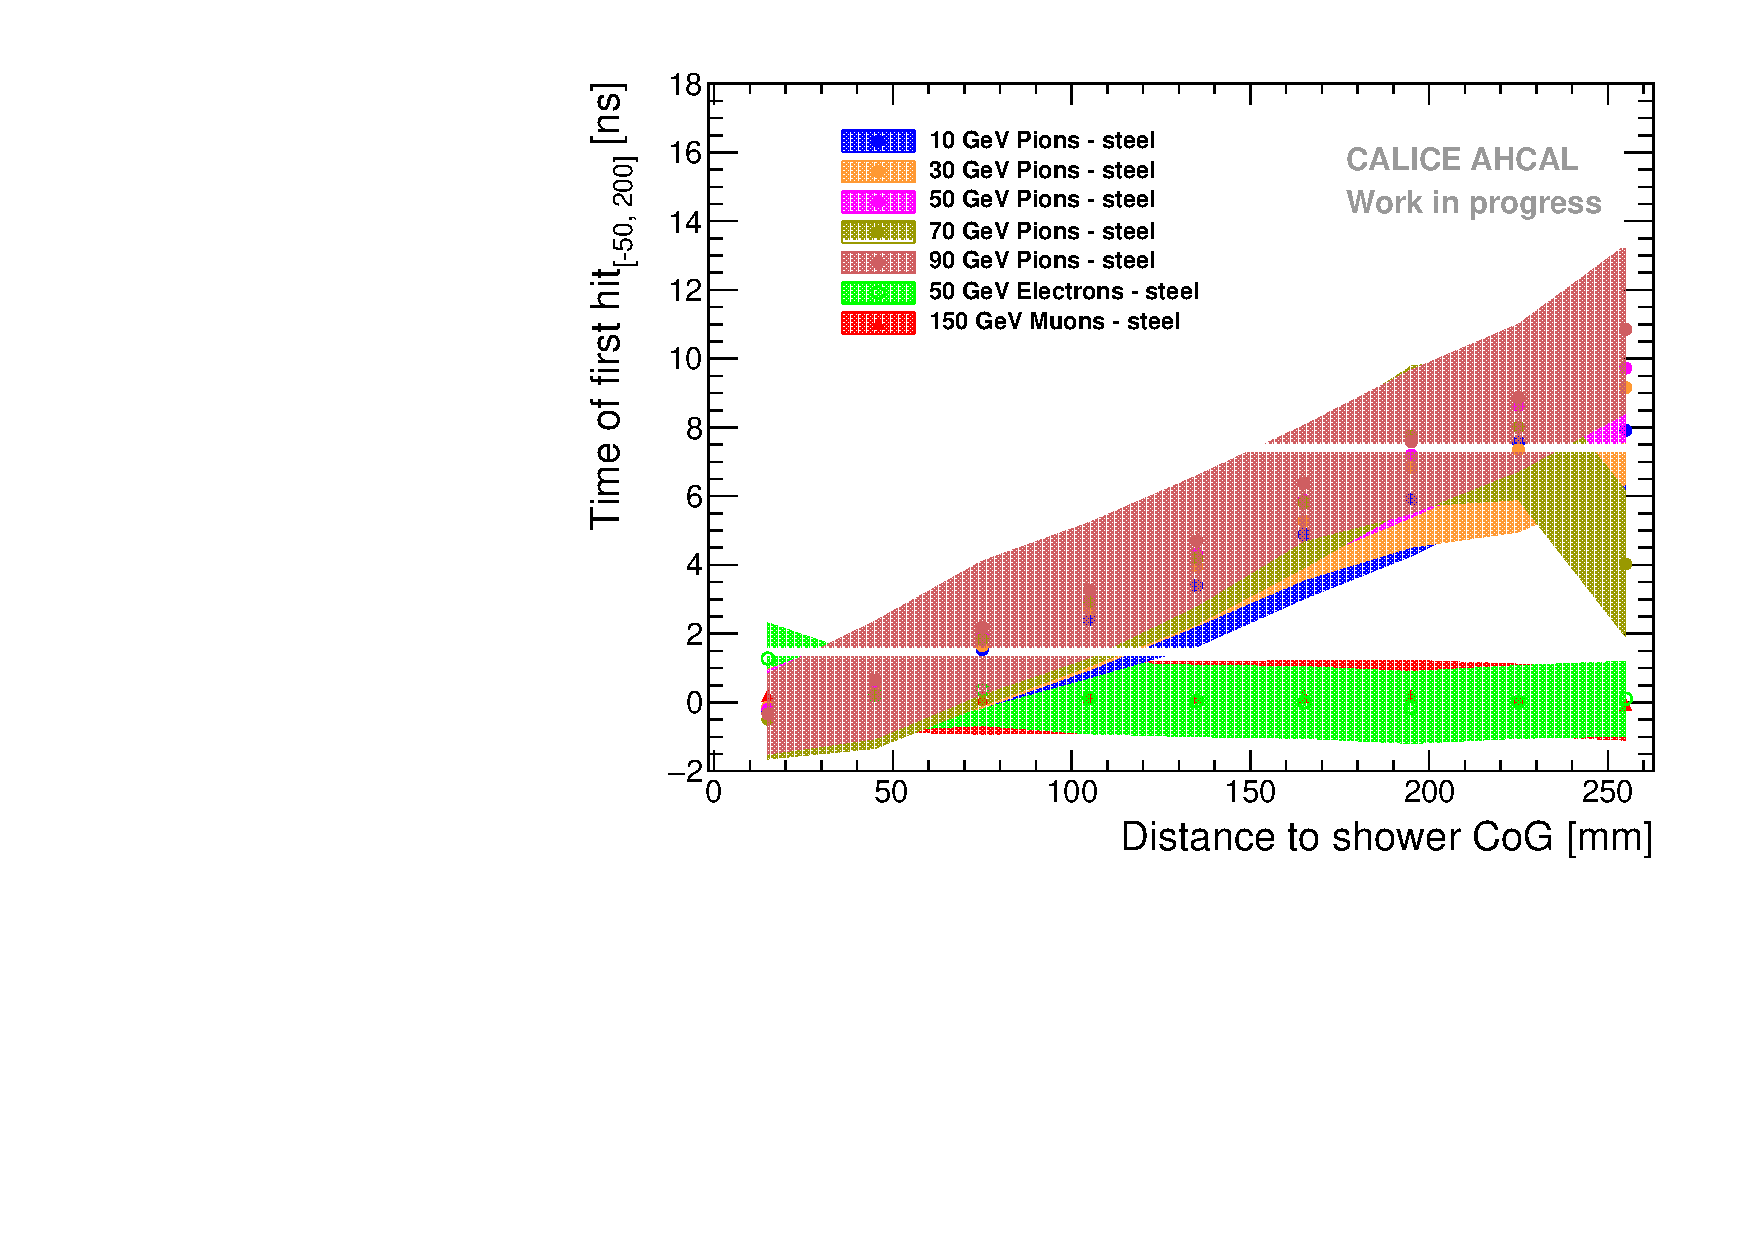
\includegraphics[width=1\textwidth]{../Thesis_Plots/Timing/Pions/Plots/Timing_Radius_Comparison_ShortAsymRange_SSF.pdf}
		\caption{Layers 3 to 10.}\label{fig:Radius_Comparison_SSF}
	\end{subfigure}
	\hfill
	\begin{subfigure}[t]{0.49\textwidth}
		\centering
		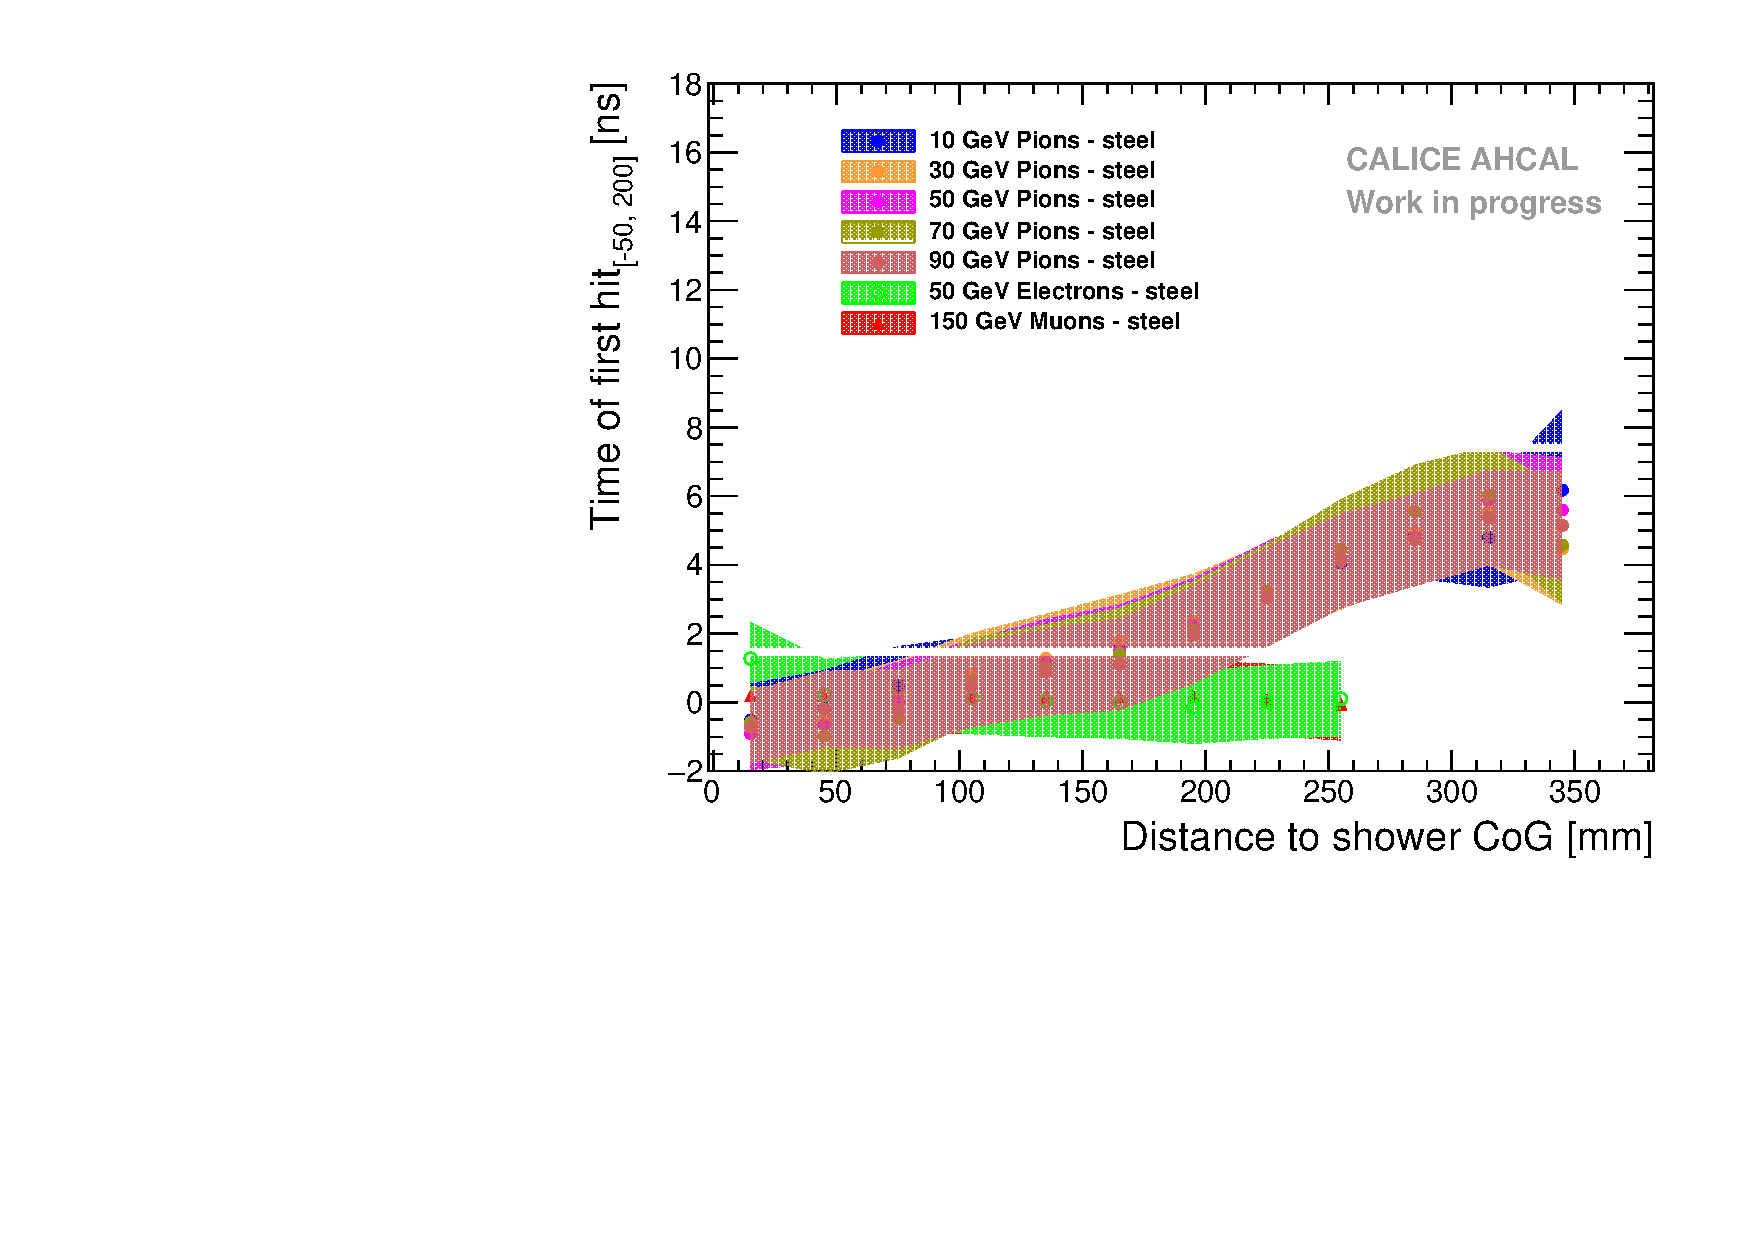
\includegraphics[width=1\textwidth]{../Thesis_Plots/Timing/Pions/Plots/Timing_Radius_Comparison_ShortAsymRange_BL.pdf}
		\caption{Layers 11 to 14.}\label{fig:Radius_Comparison_BL}
	\end{subfigure}
	\caption{Radial shower timing profile of the time of first hit for muon, electron and pion beams. The left plot shows the timing profile for the layers 3 to 10 and the right profile shows the timing profile for the layers 11 to 14. The reason for the separation is described in the text. The systematics are shown by the color bands.}
	\label{fig:RadialTiming}
\end{figure}

For muons and electrons, the mean time of the first hit does not vary with the increase of radius showing that the processes involved are prompt and independent of the position. On the contrary for hadronic showers, it shows an increase of the mean time of the first hit as function of the hit distance to the shower axis. As well, there is no dependence on the energy of the shower. However, the layers 3 to 10 present a steeper slope by around 50\% than for the layers 11 to 14 (from $\sim$1 ns per tile to $\sim$0.5 ns per tile).

Nevertheless, the observation is consistent with the expectation of the core of the shower depositing promptly most of the energy via EM sub-showers and relativistic particles near the shower axis. This is followed by a hadronic halo which contributes to delayed signals that may be from mainly neutron-induced processes. For the layers 3 to 10, the mean time of first hit varies between 0 ns at small radius and 10 ns at 25 cm. For the layers 11 to 14, it varies between 0 ns near the shower axis, 4 ns at 25 cm and 6 ns at 35 cm.

\begin{figure}[htbp!]
	\begin{subfigure}[t]{0.49\textwidth}
		\centering
		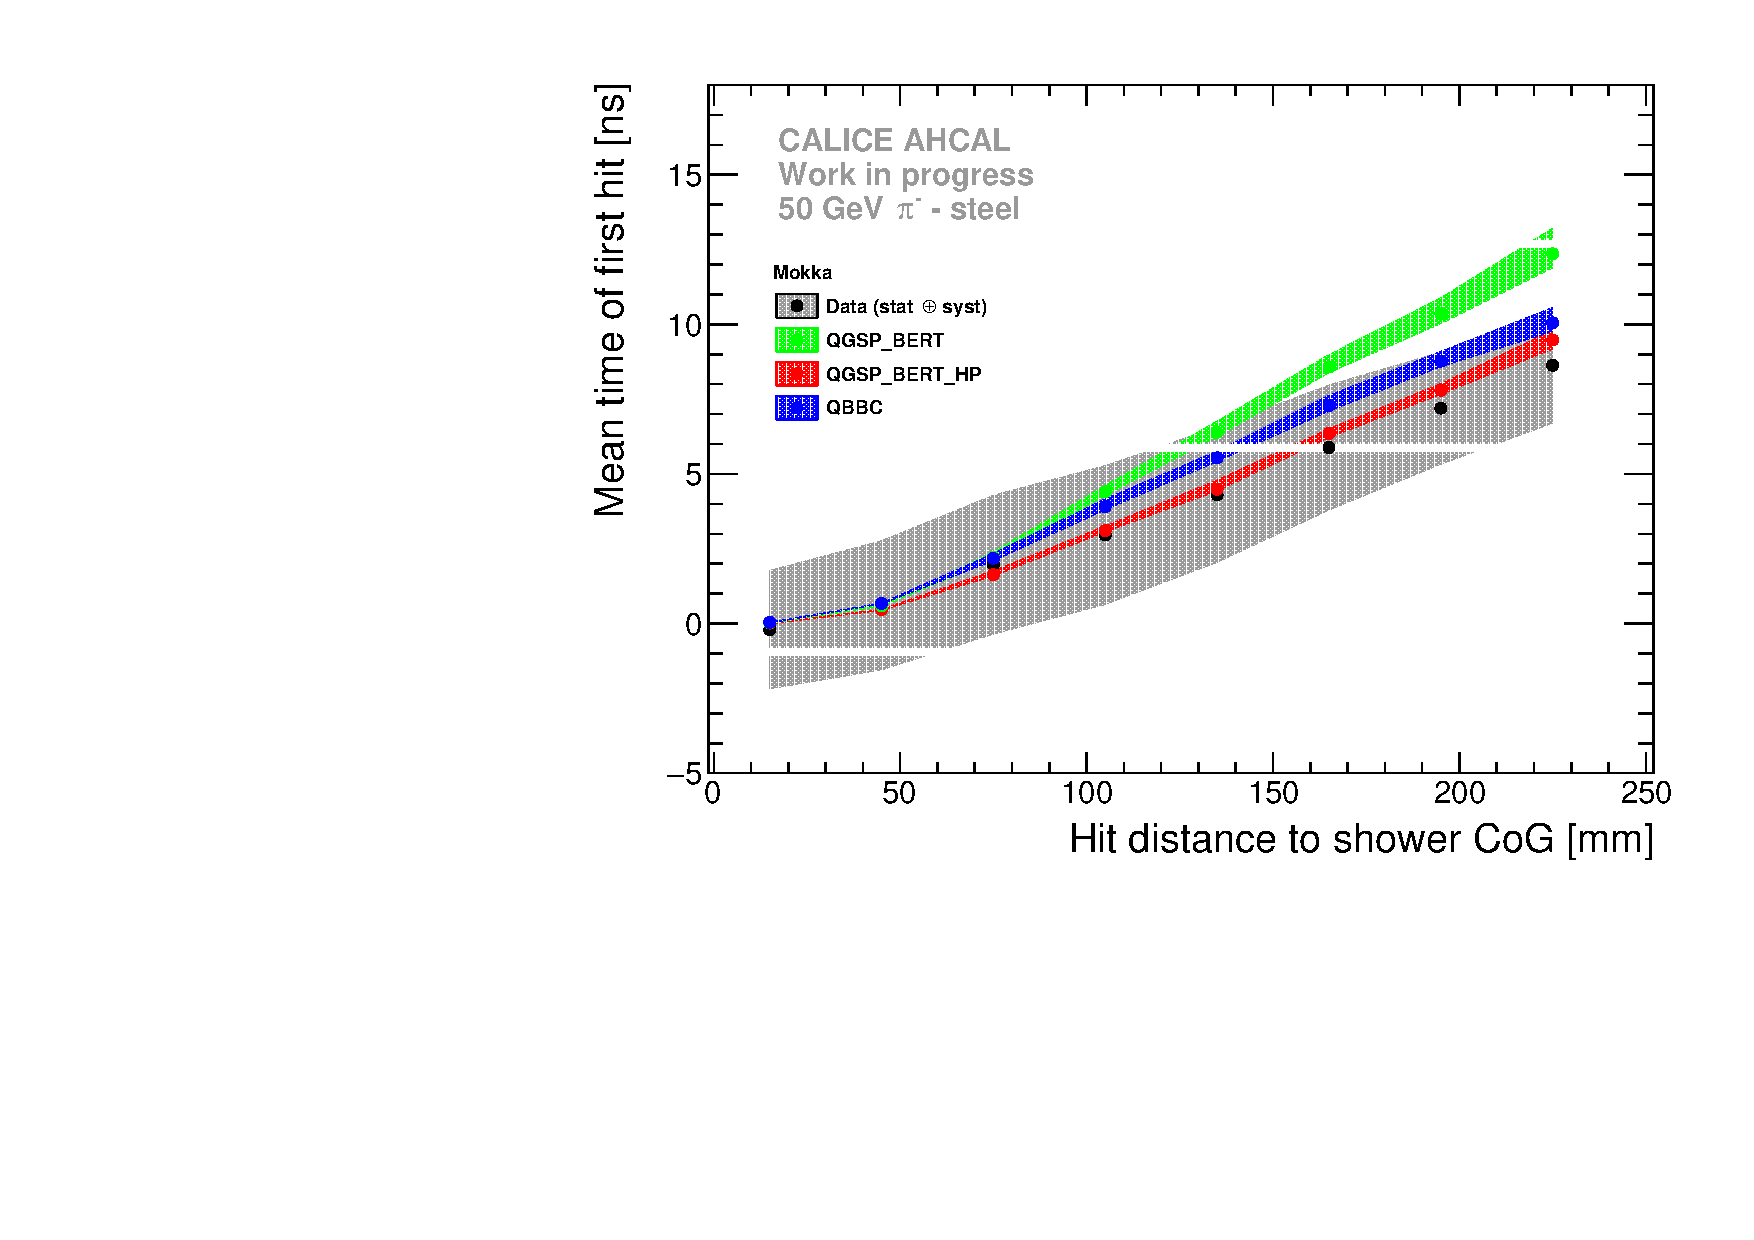
\includegraphics[width=1\textwidth]{../Thesis_Plots/Timing/Pions/Plots/ComparisonToSim/Time_Radius_50GeV_SSF_Mokka.pdf}
		\caption{Layers 3 to 10} \label{fig:Radius_SSF_SimData_50GeV}
	\end{subfigure}
	\hfill
	\begin{subfigure}[t]{0.49\textwidth}
		\centering
		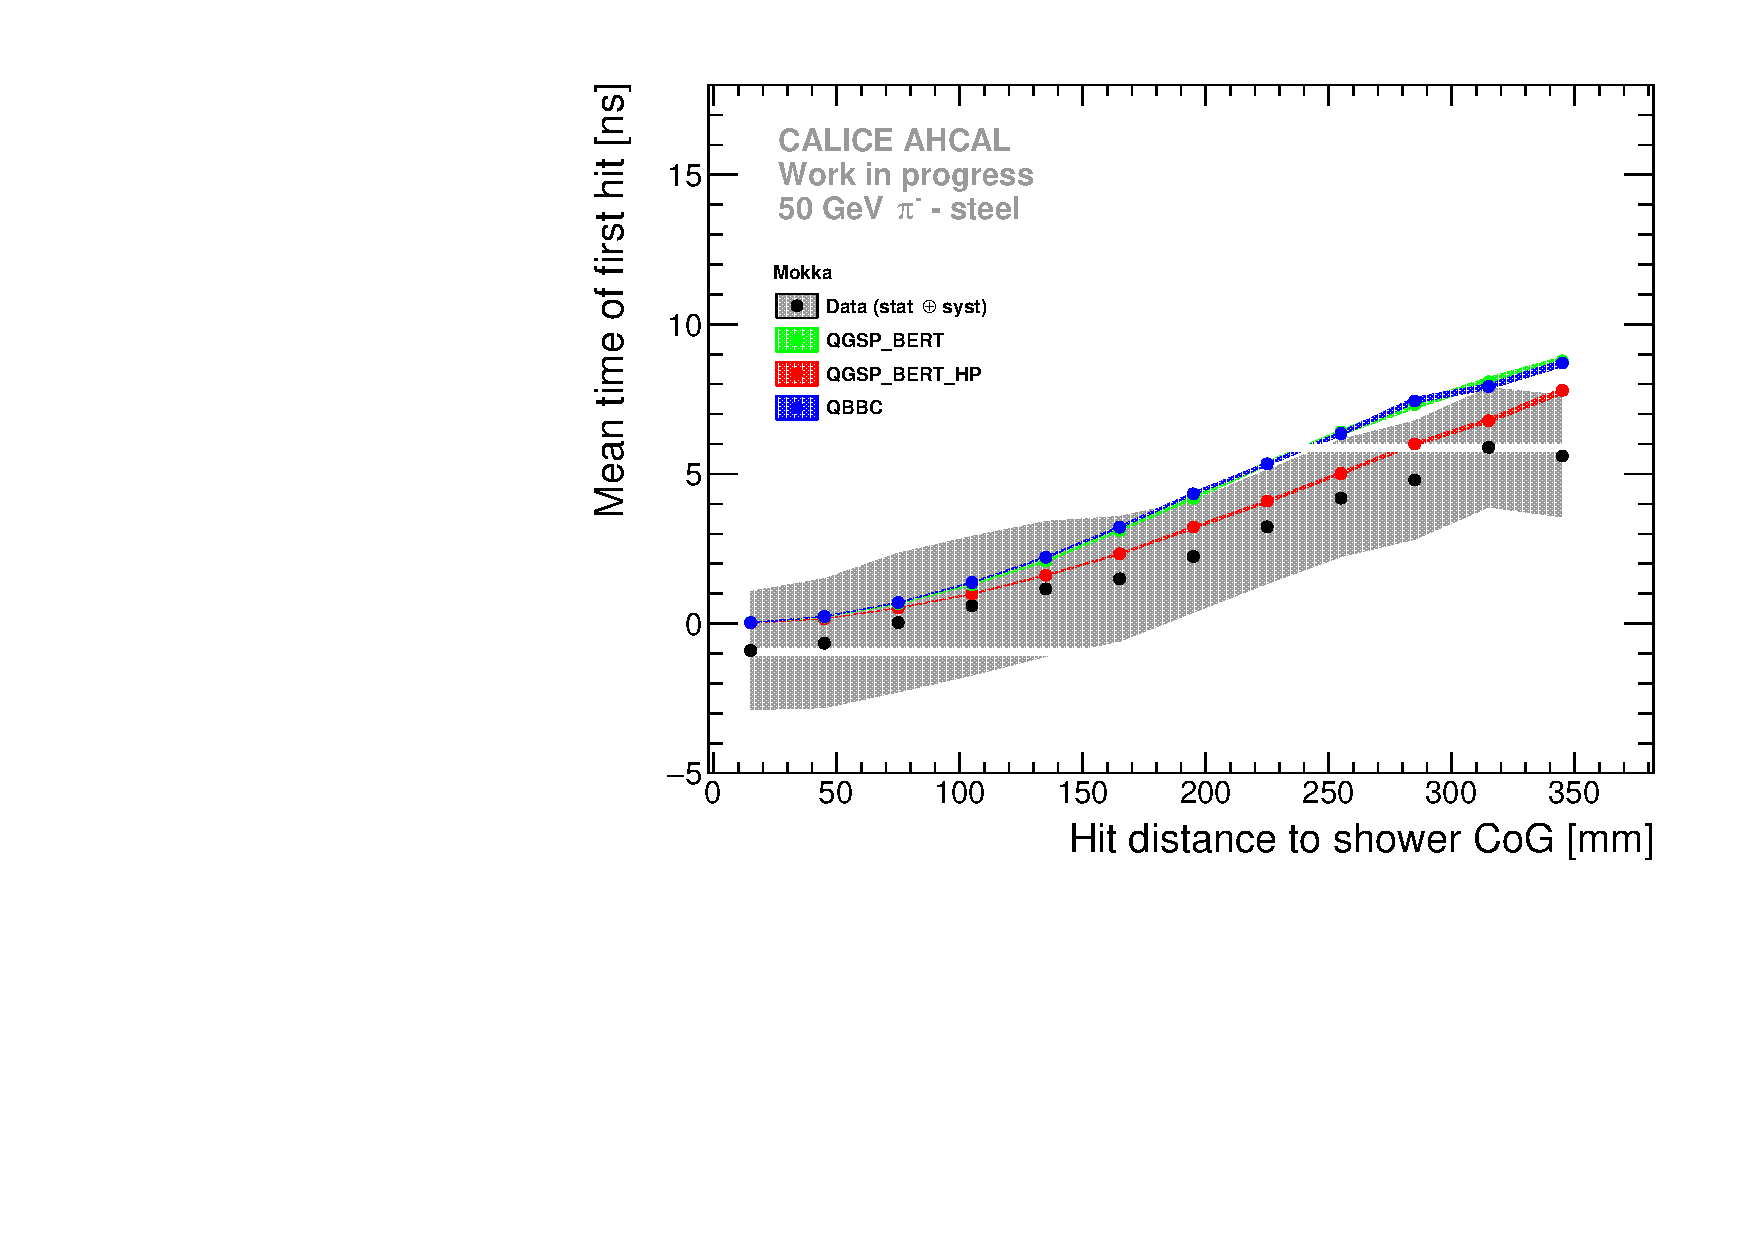
\includegraphics[width=1\textwidth]{../Thesis_Plots/Timing/Pions/Plots/ComparisonToSim/Time_Radius_50GeV_BL_Mokka.pdf}
		\caption{Layers 11 to 14} \label{fig:Radius_BL_SimData_50GeV}
	\end{subfigure}
	\caption{Comparison of the time of first hit as function of the hit distance to the shower axis in data and \mokka simulation for 50 GeV pion for the layers 3 to 10 on the left and for layers 11 to 14 on the right. The grey and color bands shows the systematics.}
	\label{fig:Radius_SSF_SimData_50GeVComparison}
\end{figure}

The radial dependence of the time of first hit of 50 GeV pion showers is compared to simulations as shown in figure \ref{fig:Radius_SSF_SimData_50GeVComparison}. For other energies and simulations, the figures can be seen in appendix \ref{appendix:TimingAdd}. For the layers 3 to 10, the QBBC and QGSP\_BERT\_HP physics lists reproduce well the data within systematics. The QGSP\_BERT physics list agrees well under a 10 cm distance and then starts to deviate from data up to 4-6 ns at 23 cm. Concerning the layers 11 to 14, over the full energy range, the QGSP\_BERT\_HP physics list agrees the best with the data. The QBBC and QGSP\_BERT physics lists agree with data up to around a 10 cm distance and then both lie above the data for higher distances, varying between few ns to 3-4 ns between 17 cm to 35 cm distance. This study shows that without the precision neutron tracking in simulation, too many late energy depositions are created that are spread far away from the shower axis.

\subsection{Time dependence with the shower depth}
\label{sec:TimeRadiusDepth}

The dependence of the mean time of first hit as function of the hit distance to the center of gravity of the shower for different layers, i.e. corresponding to different shower depths, is shown in figure \ref{fig:Radius_Indivi}. One can notice that there is a dependency of the slope of the curve as function of the layer. Layer 3 shows a much steeper slope of around 1.8 ns per tile than for the layer 14 at 0.6 ns per tile. The study has been compared to simulation with the QGSP\_BERT\_HP physics list as well and the same behavior is described by the simulation as shown in figure \ref{fig:Radius_Indivi_Sim}. In simulation, the layer 3 shows a slope of around 1.7 ns per tile and the layer 14 show a slope of 0.5 ns per tile. This dependency is not fully understood and seems counter intuitive as one would expect more later hits in the last layers. One possibility is that the late component for the first layers could come from the Albedo effect \cite{ELLSWORTH1982167} and backscattered neutrons.

\begin{figure}[htbp!]
	\begin{subfigure}[t]{0.49\textwidth}
		\centering
		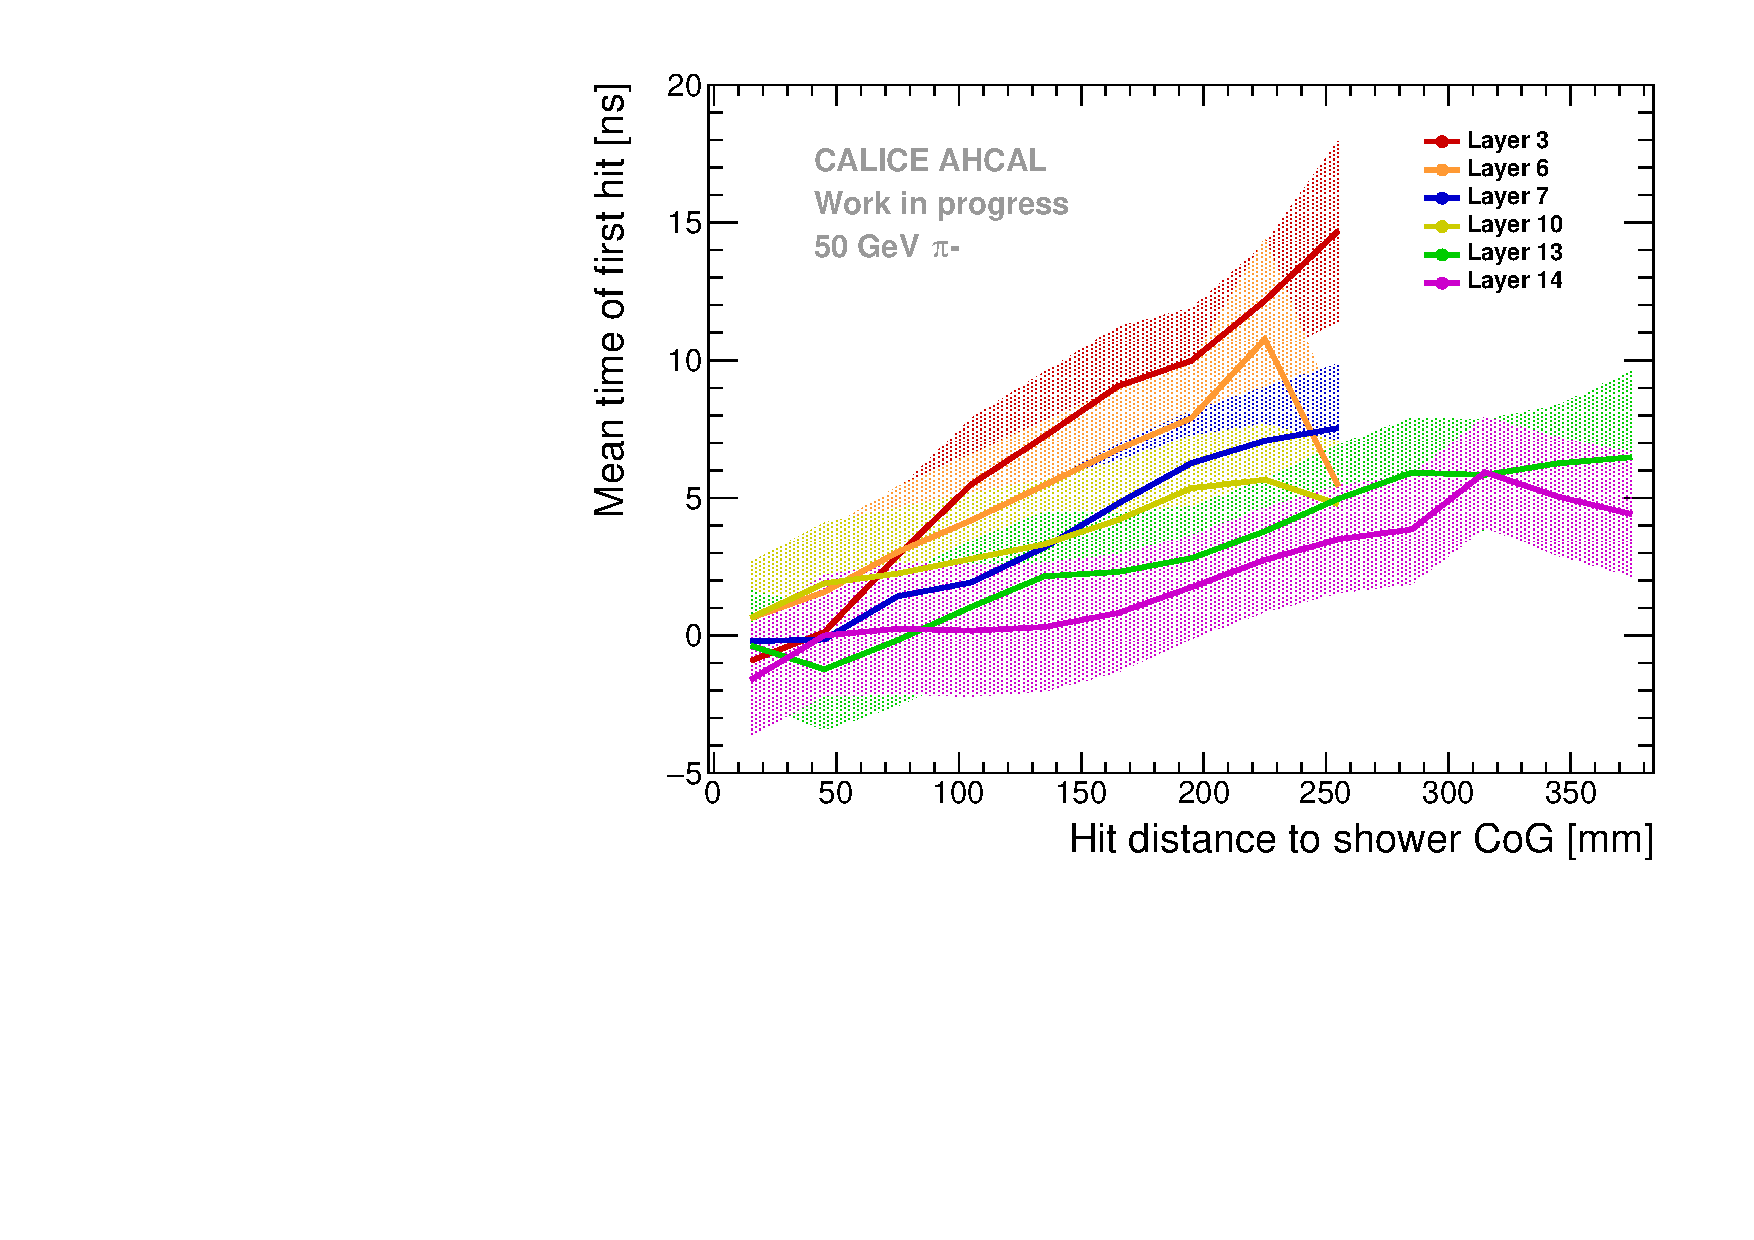
\includegraphics[width=1\textwidth]{../Thesis_Plots/Timing/Pions/Plots/Timing_Radius_Comparison_ShortAsymRange_IndividualLayers.pdf}
		\caption{}\label{fig:Radius_Indivi}
	\end{subfigure}
	\hfill
	\begin{subfigure}[t]{0.49\textwidth}
		\centering
		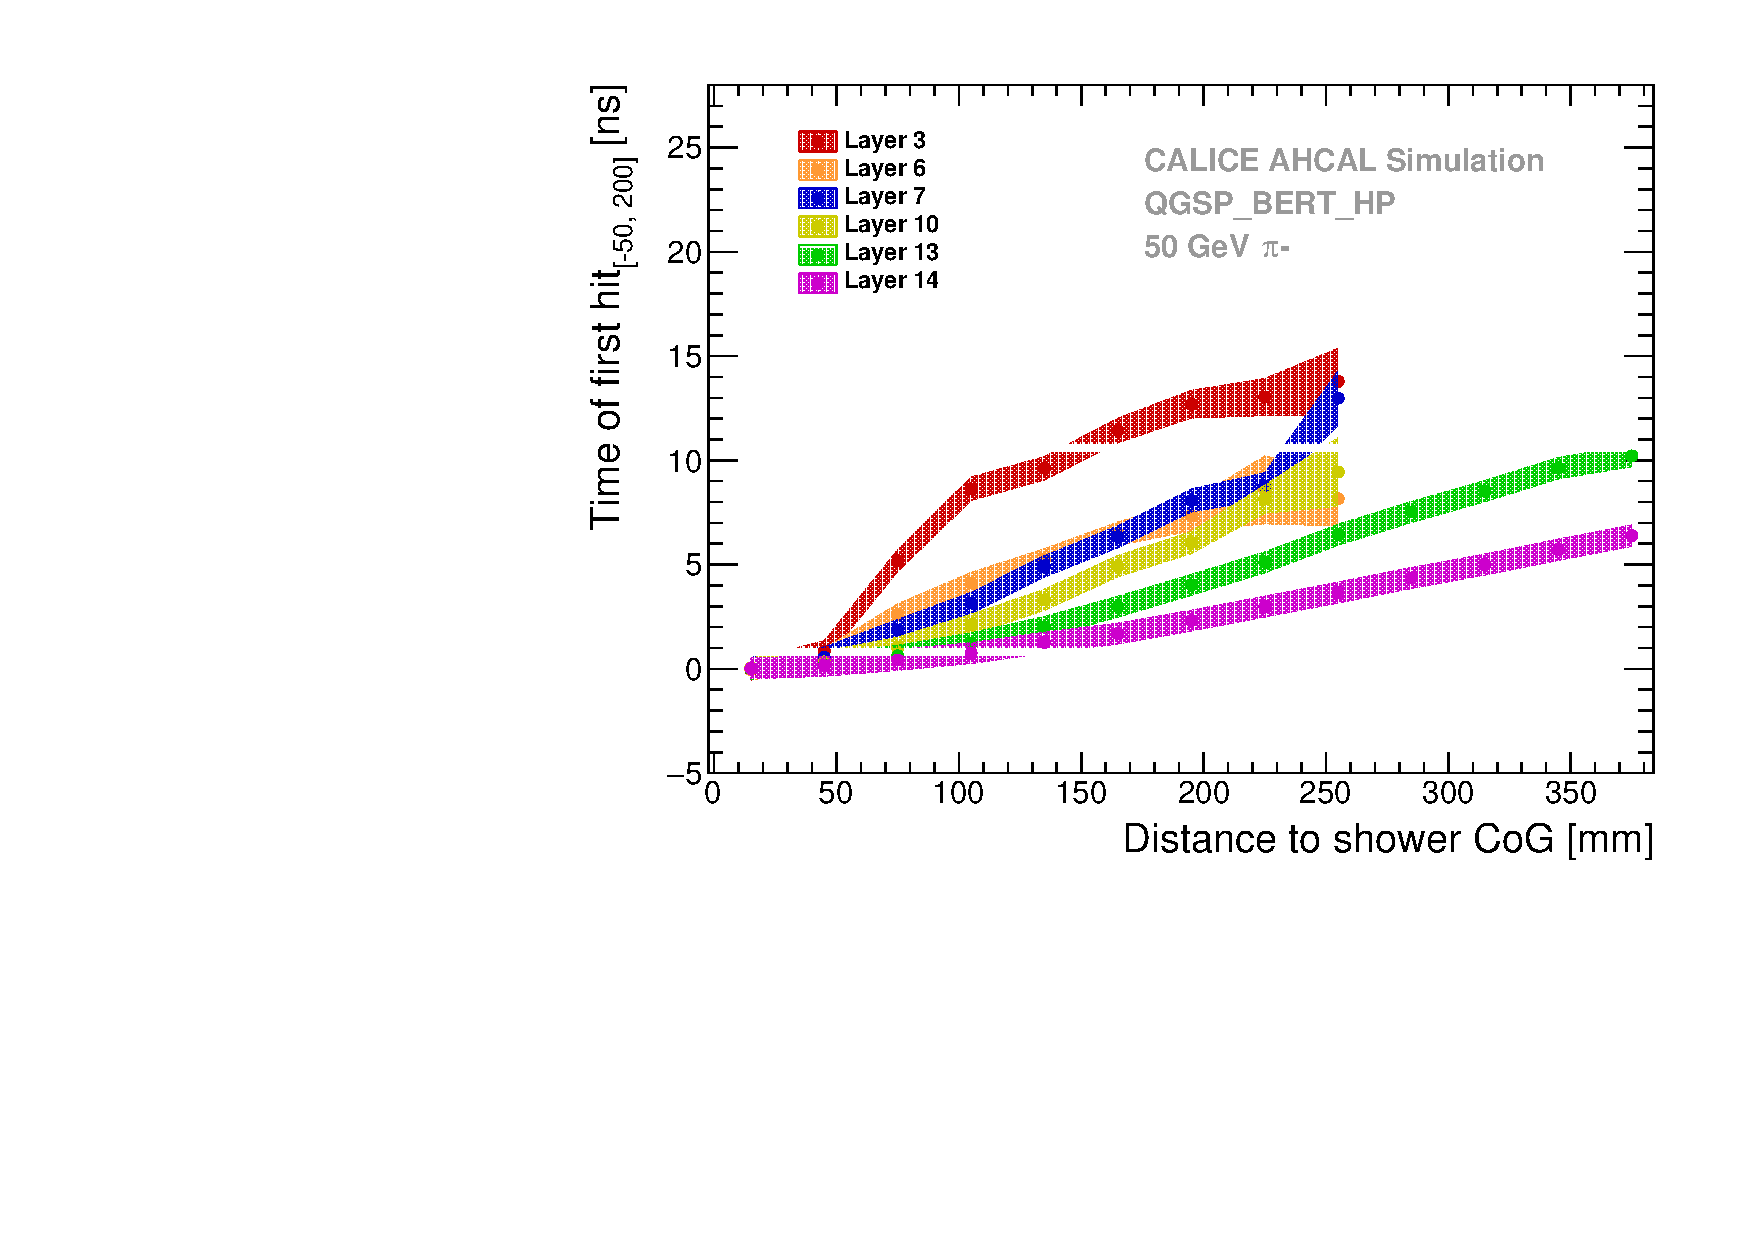
\includegraphics[width=1\textwidth]{../Thesis_Plots/Timing/Pions/Plots/Timing_Radius_Comparison_ShortAsymRange_IndividualLayers_Sim.pdf}
		\caption{}\label{fig:Radius_Indivi_Sim}
	\end{subfigure}
	\caption{Mean time of first hit as function of the hit distance to the center of gravity for 50 GeV pions for different layers. On the left, it is shown for data. On the right, it is shown for simulation using the QGSP\_BERT\_HP physics list. Both figures shows the same behavior with a decrease of the curve slope for deeper layers in the calorimeter.}
	\label{fig:Radius_IndiviAll}
\end{figure}

To understand this effect, the mean time of first hit as a function of the hit distance to the shower axis is investigated at a constant distance between a layer and the first hard interaction (\acrshort{fhi}) layer. To do this, the shower start finder algorithm is based on previous work \cite{CaN026} in order find the layer of the first hard interaction. However, slight modifications had to be done due to the fact that some of the layers in the front of the detector show a bad performance with many non-working channels.

The basics of the algorithm is to find the primary pion track and to determine the shower start layer. To determine the shower start layer $s_{layer}$, the number of hits $n_{Hits}^{i, i+1}$ in the layer $i$ and $i+1$ is counted. If $n_{Hits}^{i, i+1} > 6$, the shower is considered started between layer $i$ and $i+1$. To determine the correct layer, the energy sum between layer $i$, $i+1$, $i+2$ and $i+3$ are checked in order to determine the correct layer for the start of the shower. In the case of a layer is identified as the FHI, a cross-check on the length of the primary track is made. The length of the primary track is required to be over three hits. The performance of the algorithm is evaluated by looking at the difference between the reconstructed layer of the FHI and the Monte-Carlo truth information on the start of the shower. This is shown in figure \ref{fig:FHIAlgo}. The performance of the algorithm is good enough in order to get a good estimate of the FHI layer but it has a small tendency to reconstruct the FHI at a deeper layer.

\begin{figure}[htbp!]
	\begin{subfigure}[t]{0.49\textwidth}
		\centering
		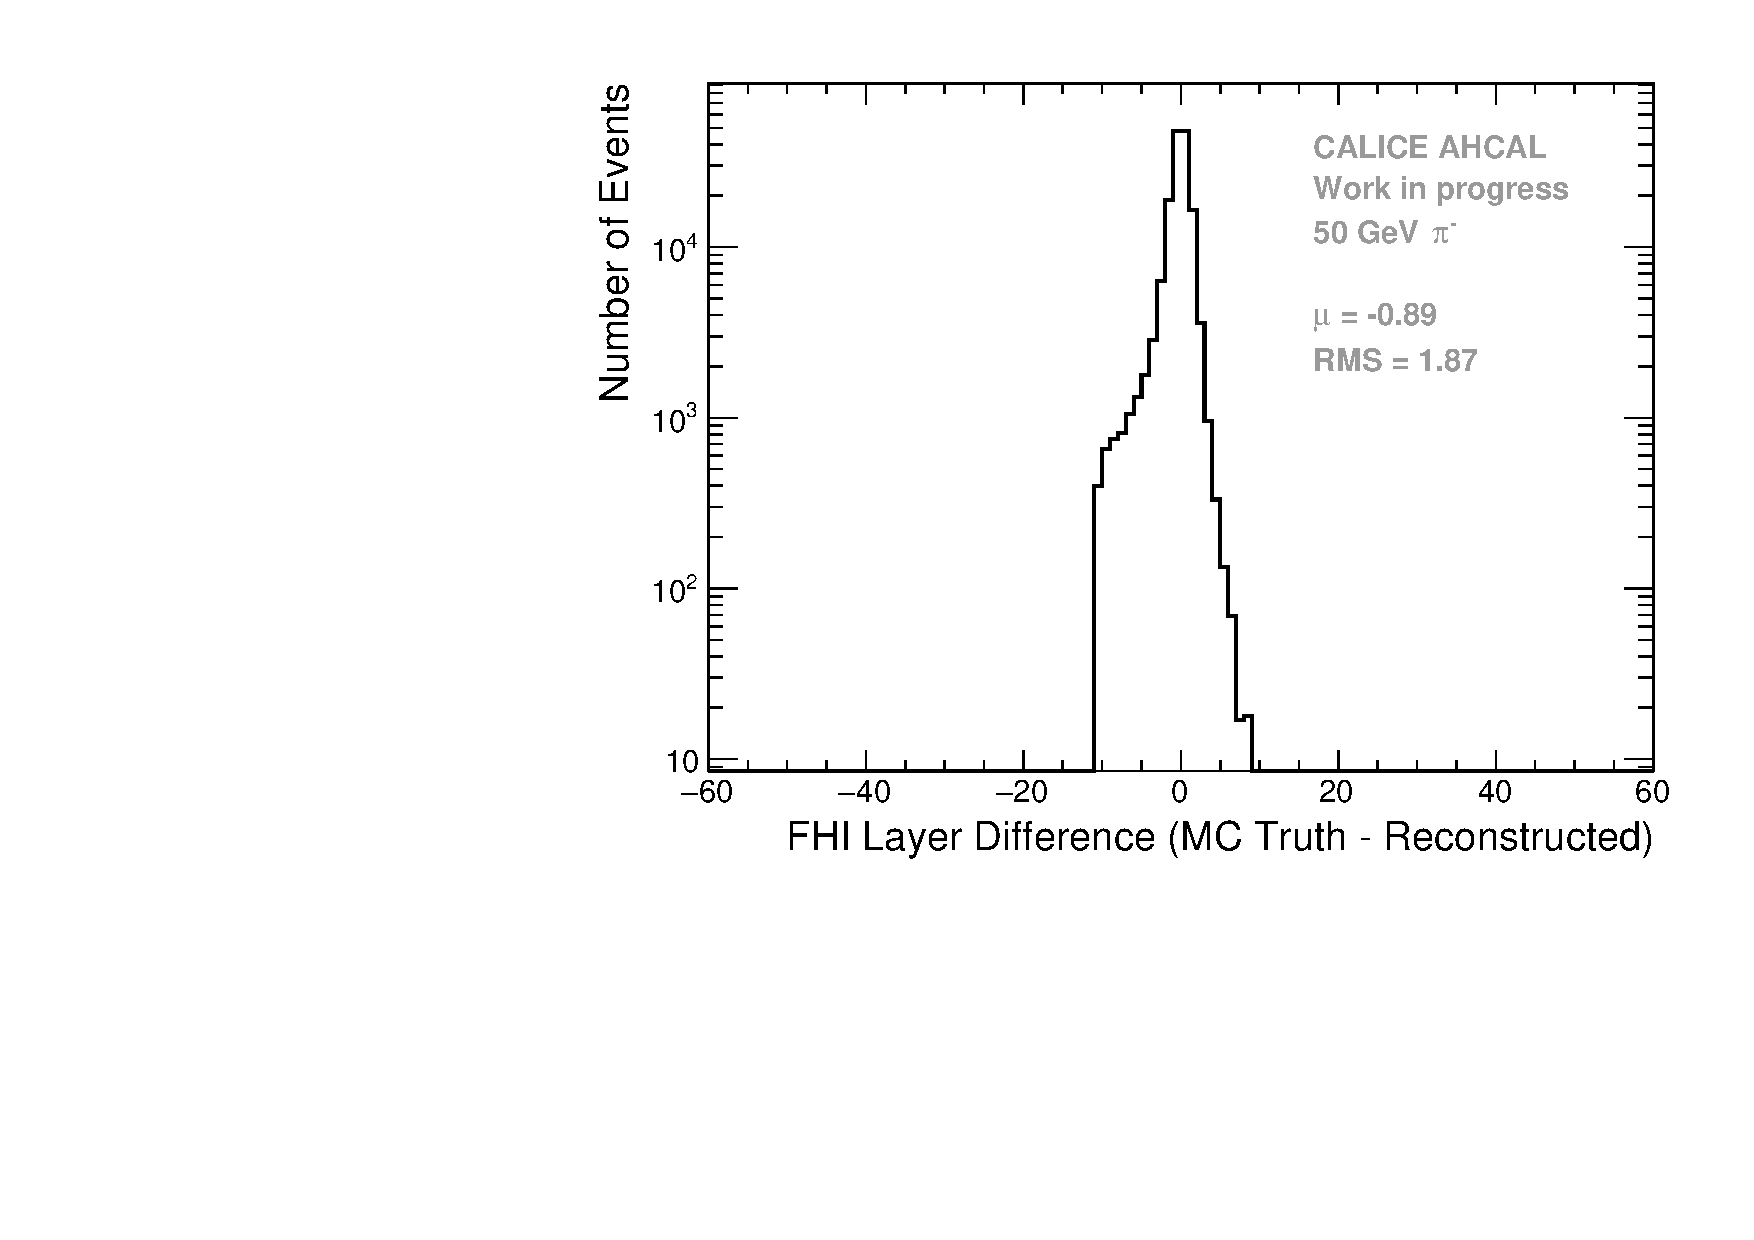
\includegraphics[width=1\textwidth]{../Thesis_Plots/Timing/Pions/Plots/ShowerStart_Difference_noOptimisation.pdf}
		\caption{}\label{fig:Diff_FHI_RecoMC}
	\end{subfigure}
	\hfill
	\begin{subfigure}[t]{0.49\textwidth}
		\centering
		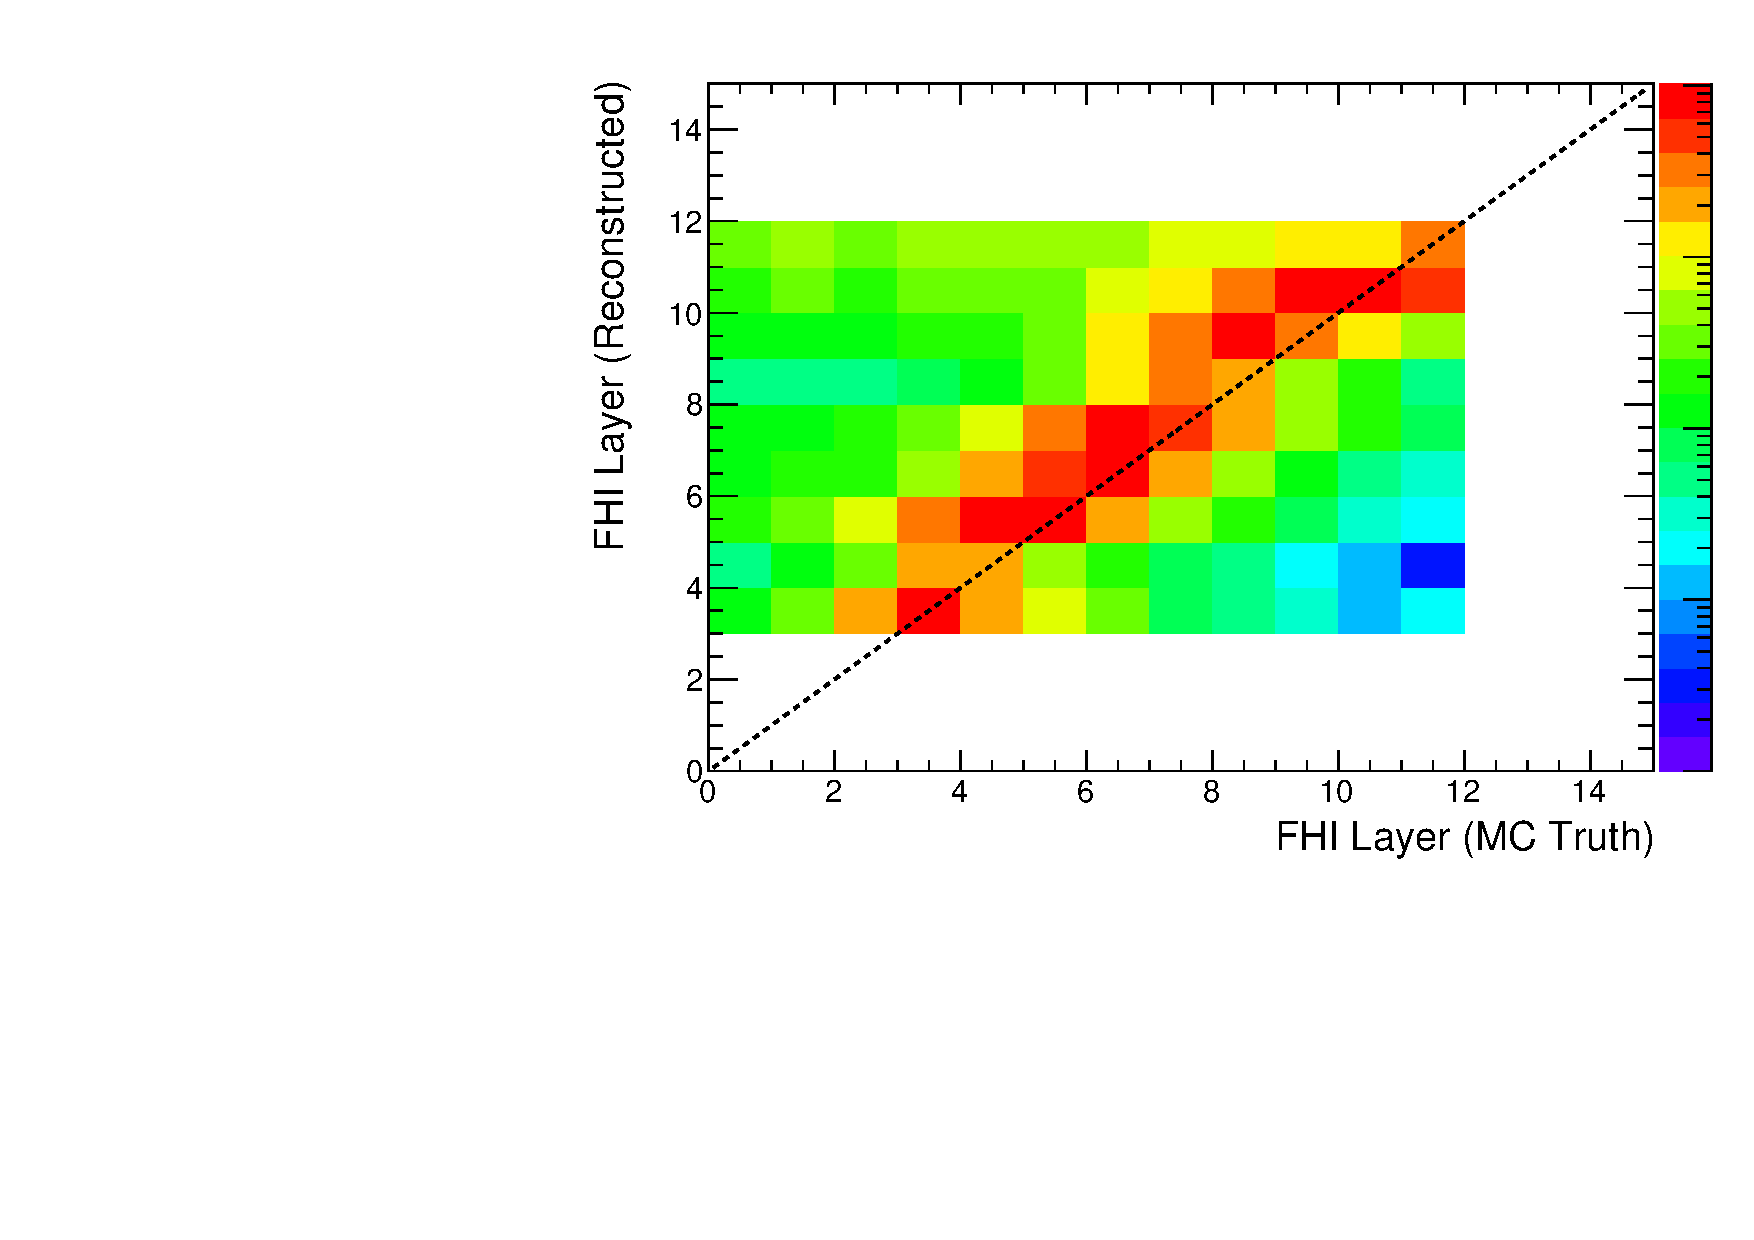
\includegraphics[width=1\textwidth]{../Thesis_Plots/Timing/Pions/Plots/ShowerStart_Difference_noOptimisation_2D.pdf}
		\caption{}\label{fig:Corr_FHI_RecoMC}
	\end{subfigure}
	\caption{Performance of the FHI algorithm in the AHCAL detector. The left plot shows the difference between the reconstructed FHI layer and the MC truth. The distribution is slightly de-centered at -0.81 with a RMS of 1.87. The right plot shows the correlation between the reconstructed FHI layer and the MC truth. The black line represent a guide for a perfect correlation.}
	\label{fig:FHIAlgo}
\end{figure}

It is expected, at a constant distance between the reconstructed FHI layer and a layer, that there will be the same dependence of the mean time of the hit as a function of the hit distance to the shower axis because in this way, the same part of the shower is sampled. Or that inversely, looking at a fixed layer, the expected behavior would be a change in the slope of the mean time of first hit as a function of the hit distance to the shower axis for different reconstructed FHI layer. The figures \ref{fig:Radius_FHI} and \ref{fig:Radius_FHI_Fixed} are an attempt for this study.

\begin{figure}[htbp!]
	\begin{subfigure}[t]{0.49\textwidth}
		\centering
		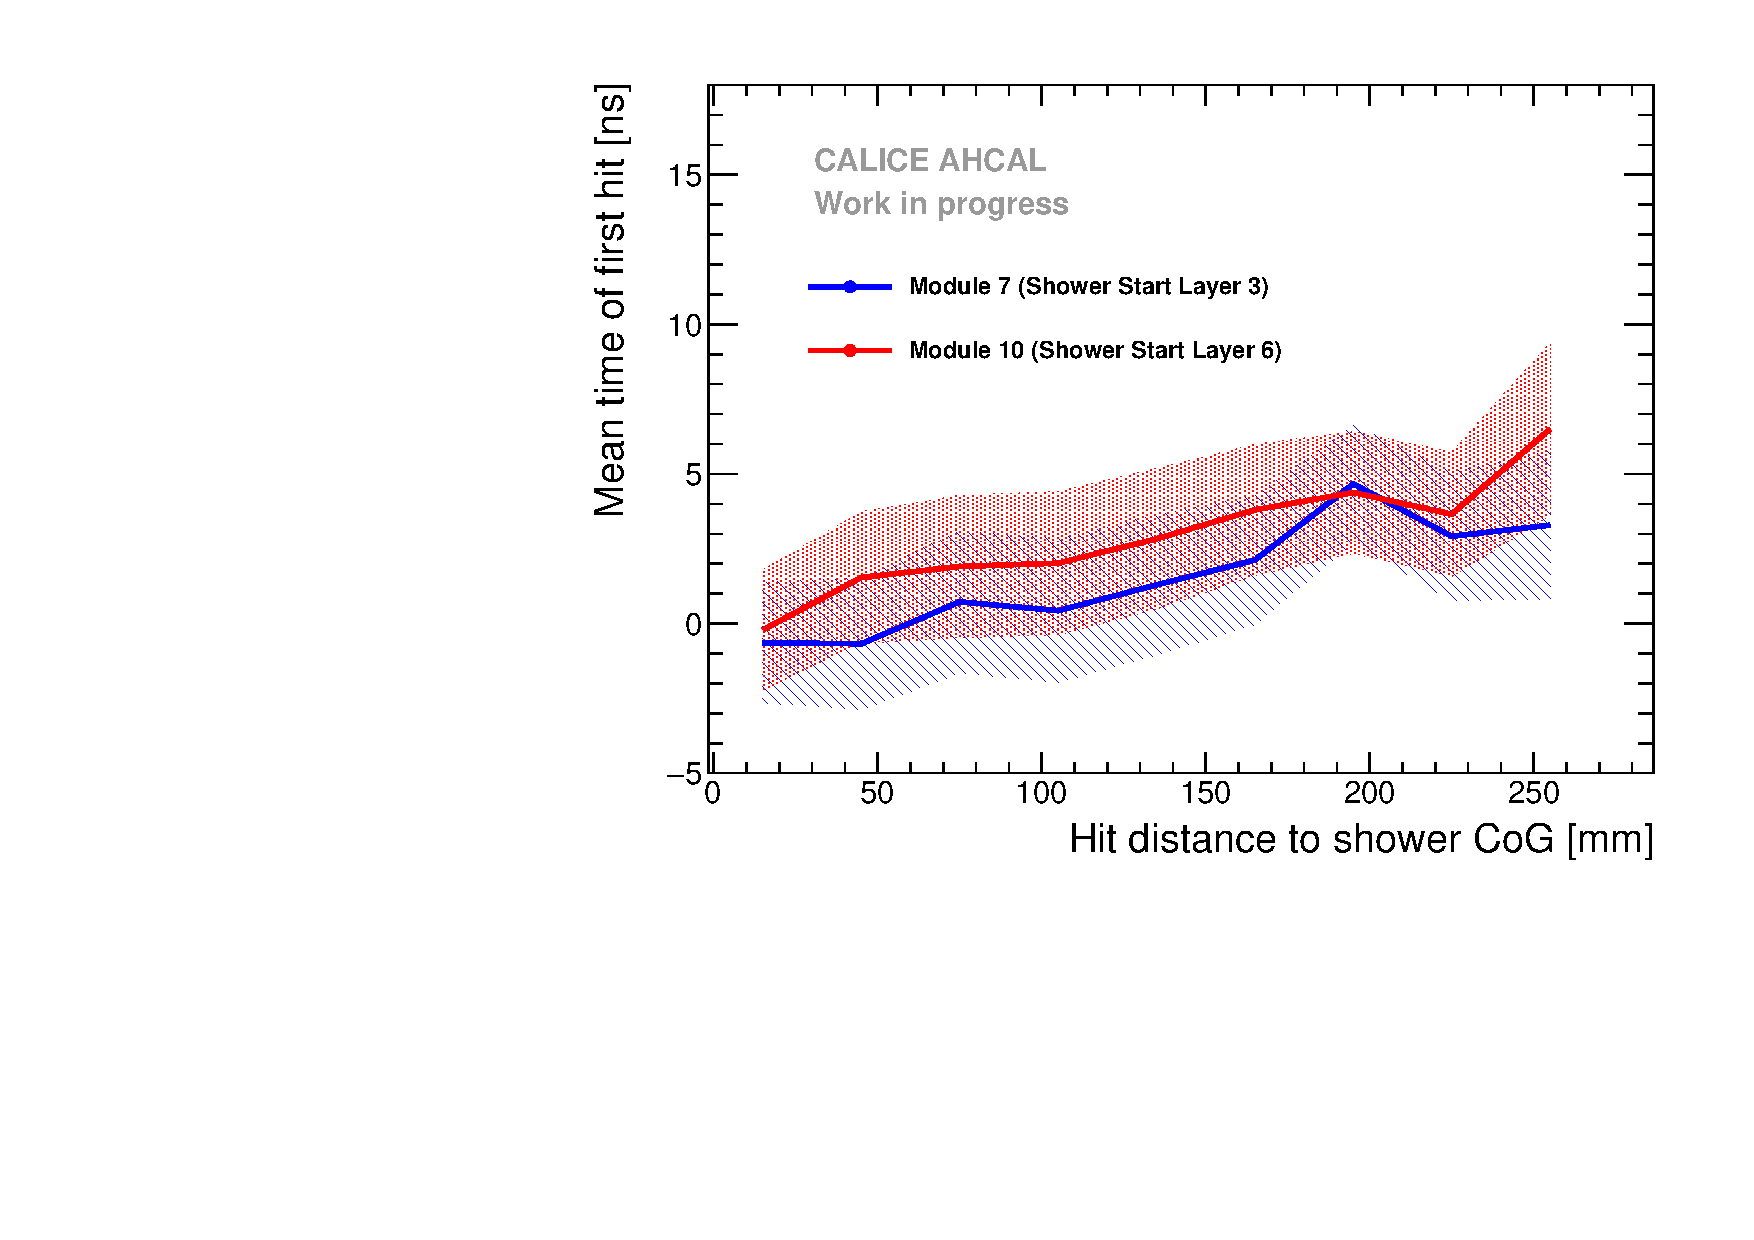
\includegraphics[width=1\textwidth]{../Thesis_Plots/Timing/Pions/Plots/Timing_Radius_Comparison_ShortAsymRange_ShowerStart.pdf}
		\caption{}\label{fig:Radius_FHI}
	\end{subfigure}
	\hfill
	\begin{subfigure}[t]{0.49\textwidth}
		\centering
		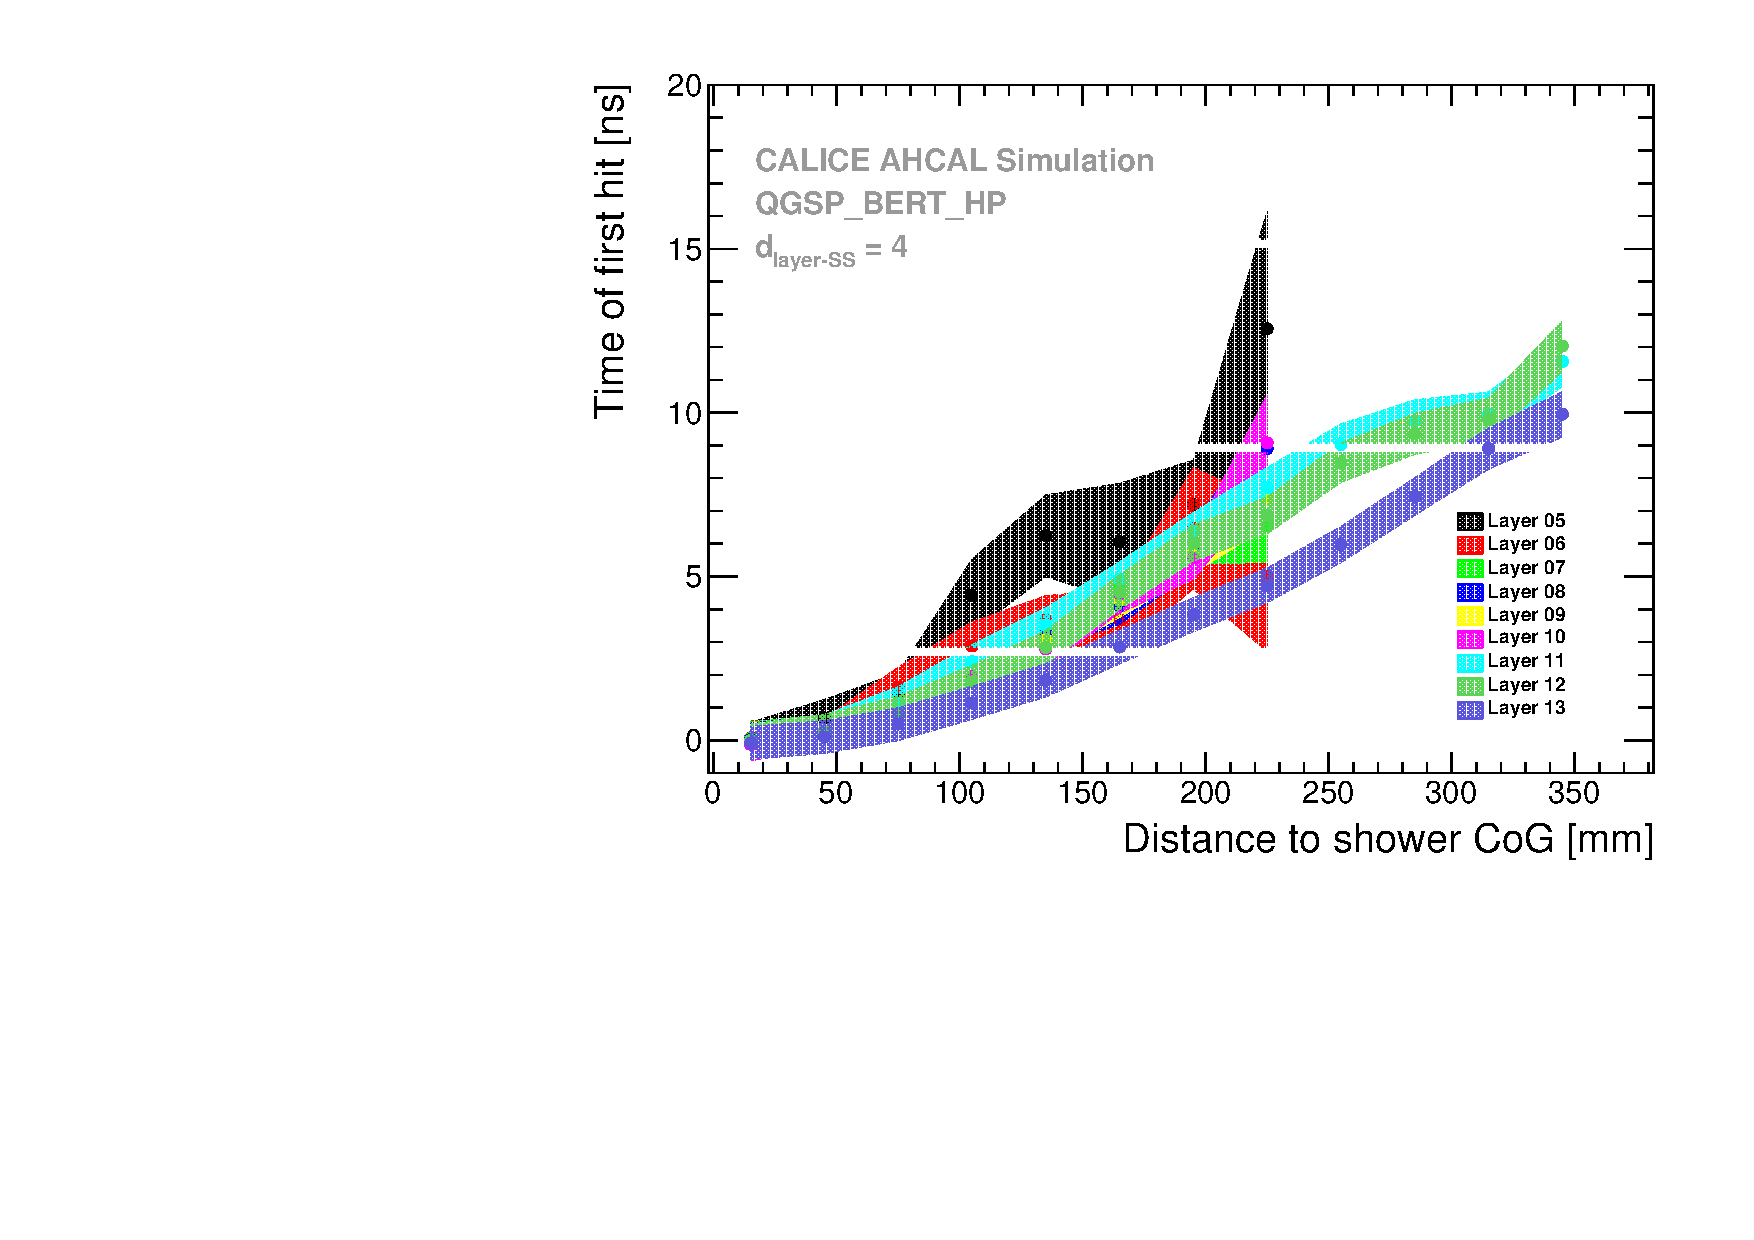
\includegraphics[width=1\textwidth]{../Thesis_Plots/Timing/Pions/Plots/Radius_ShowerStartTruth.pdf}
		\caption{}\label{fig:Radius_FHISim1}
	\end{subfigure}
	\caption{Mean time of first hit as a function of the hit distance to the shower axis for 50 GeV pions for a fixed distance of 4 between the reconstructed FHI layer and a layer. The left plot shows the radial timing profile of layer 7 and 10 in data. The right plots shows the radial timing profile for the same layers in simulation with the QGSP\_BERT\_HP physics list.}
	\label{fig:Radius_FHIAll}
\end{figure}

The data shows that by fixing the distance between the reconstructed FHI layer and a layer, the mean time of first hit displays the same slope within the systematic uncertainties. On the other hand, by looking at a fixed layer, which is in this case the layer 10, it seems that there is a trend of an increase of the curve slope as a function of the reconstructed FHI layer within the systematics. However, because of many layers not working well, it is difficult to find a different comparable configurations to confirm the observation made. In addition, a reduction of the systematic uncertainty is needed. This has been checked in simulation with the QGSP\_BERT\_HP physics list as shown in figures \ref{fig:Radius_FHISim1} and \ref{fig:Radius_FHI_FixedSim}. The simulation agrees well with the observation made in the data.

\begin{figure}[htbp!]
	\begin{subfigure}[t]{0.49\textwidth}
		\centering
		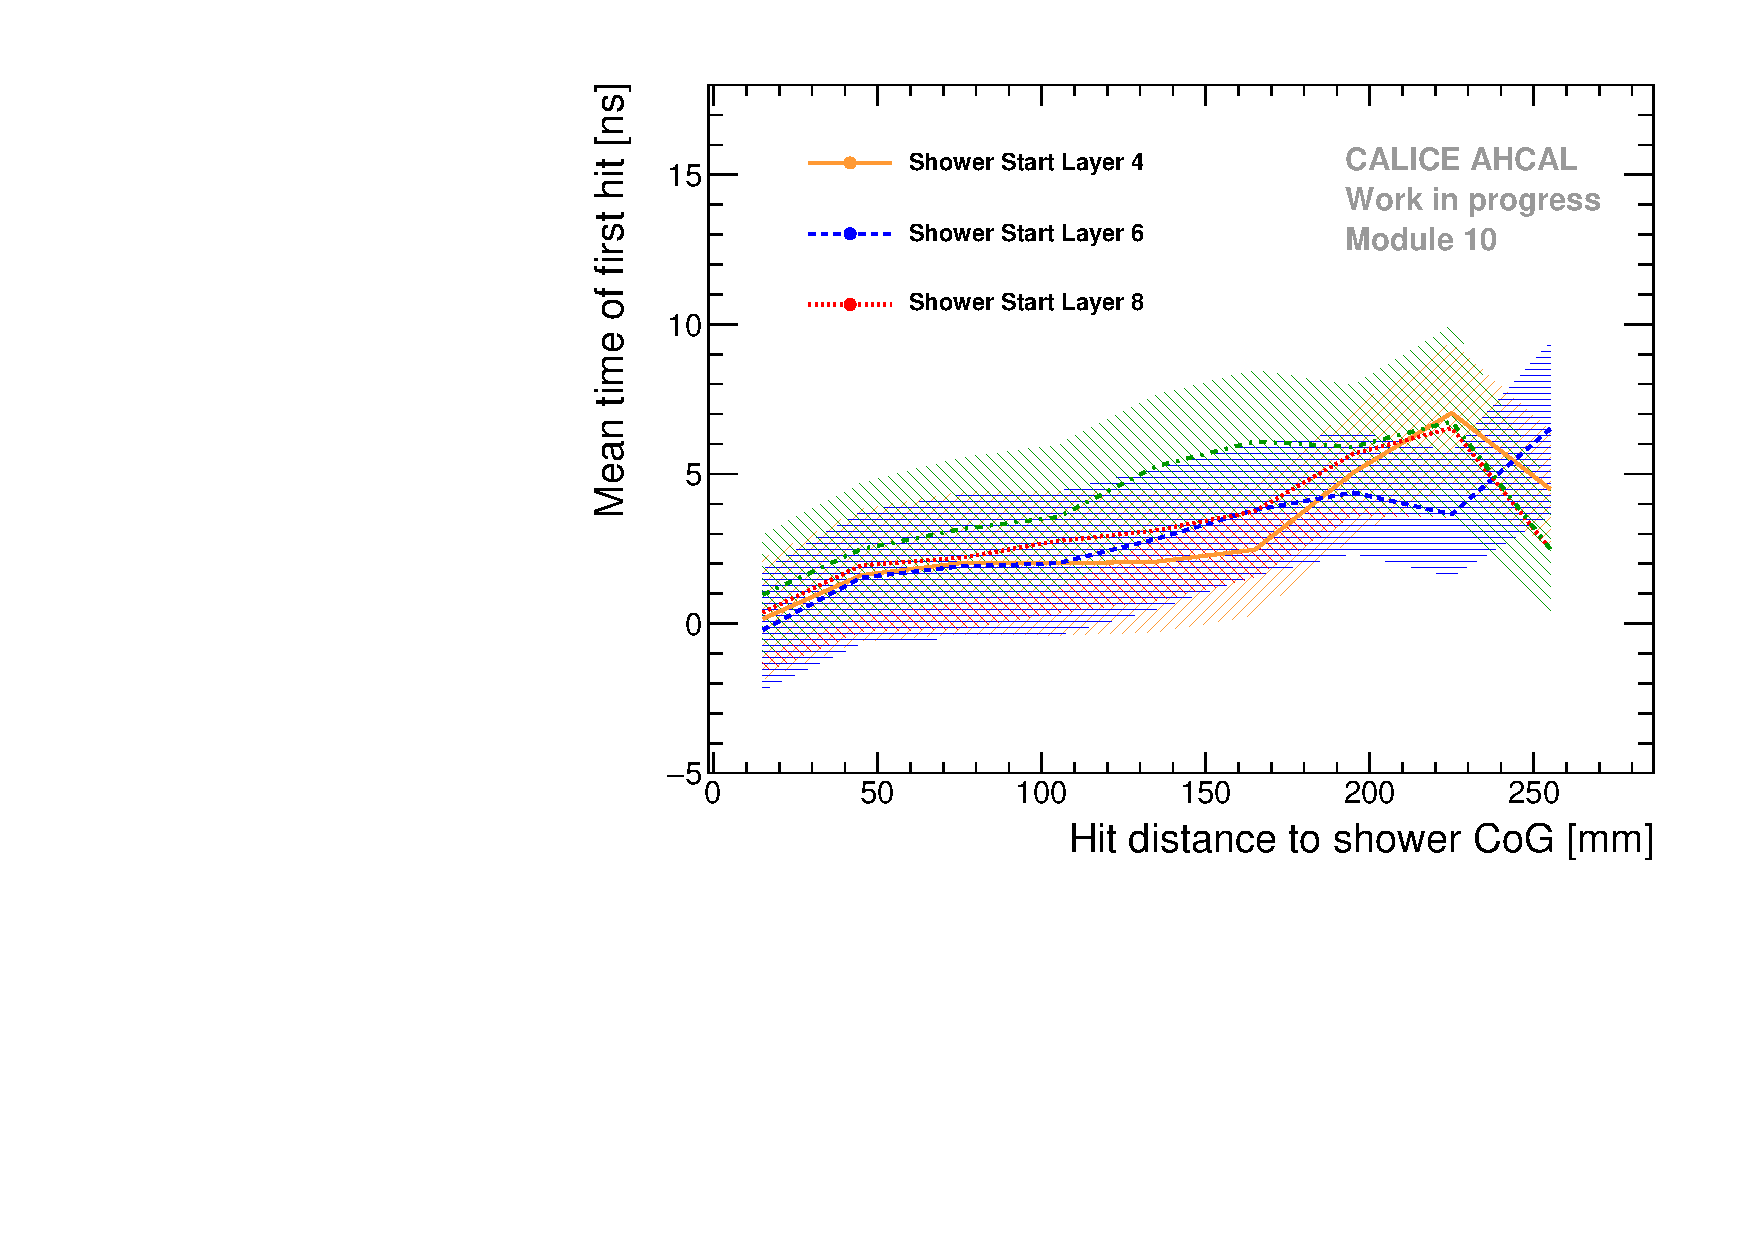
\includegraphics[width=1\textwidth]{../Thesis_Plots/Timing/Pions/Plots/Timing_Radius_Comparison_ShortAsymRange_ShowerStart_FixedModule.pdf}
		\caption{}\label{fig:Radius_FHI_Fixed}
	\end{subfigure}
	\hfill
	\begin{subfigure}[t]{0.49\textwidth}
		\centering
		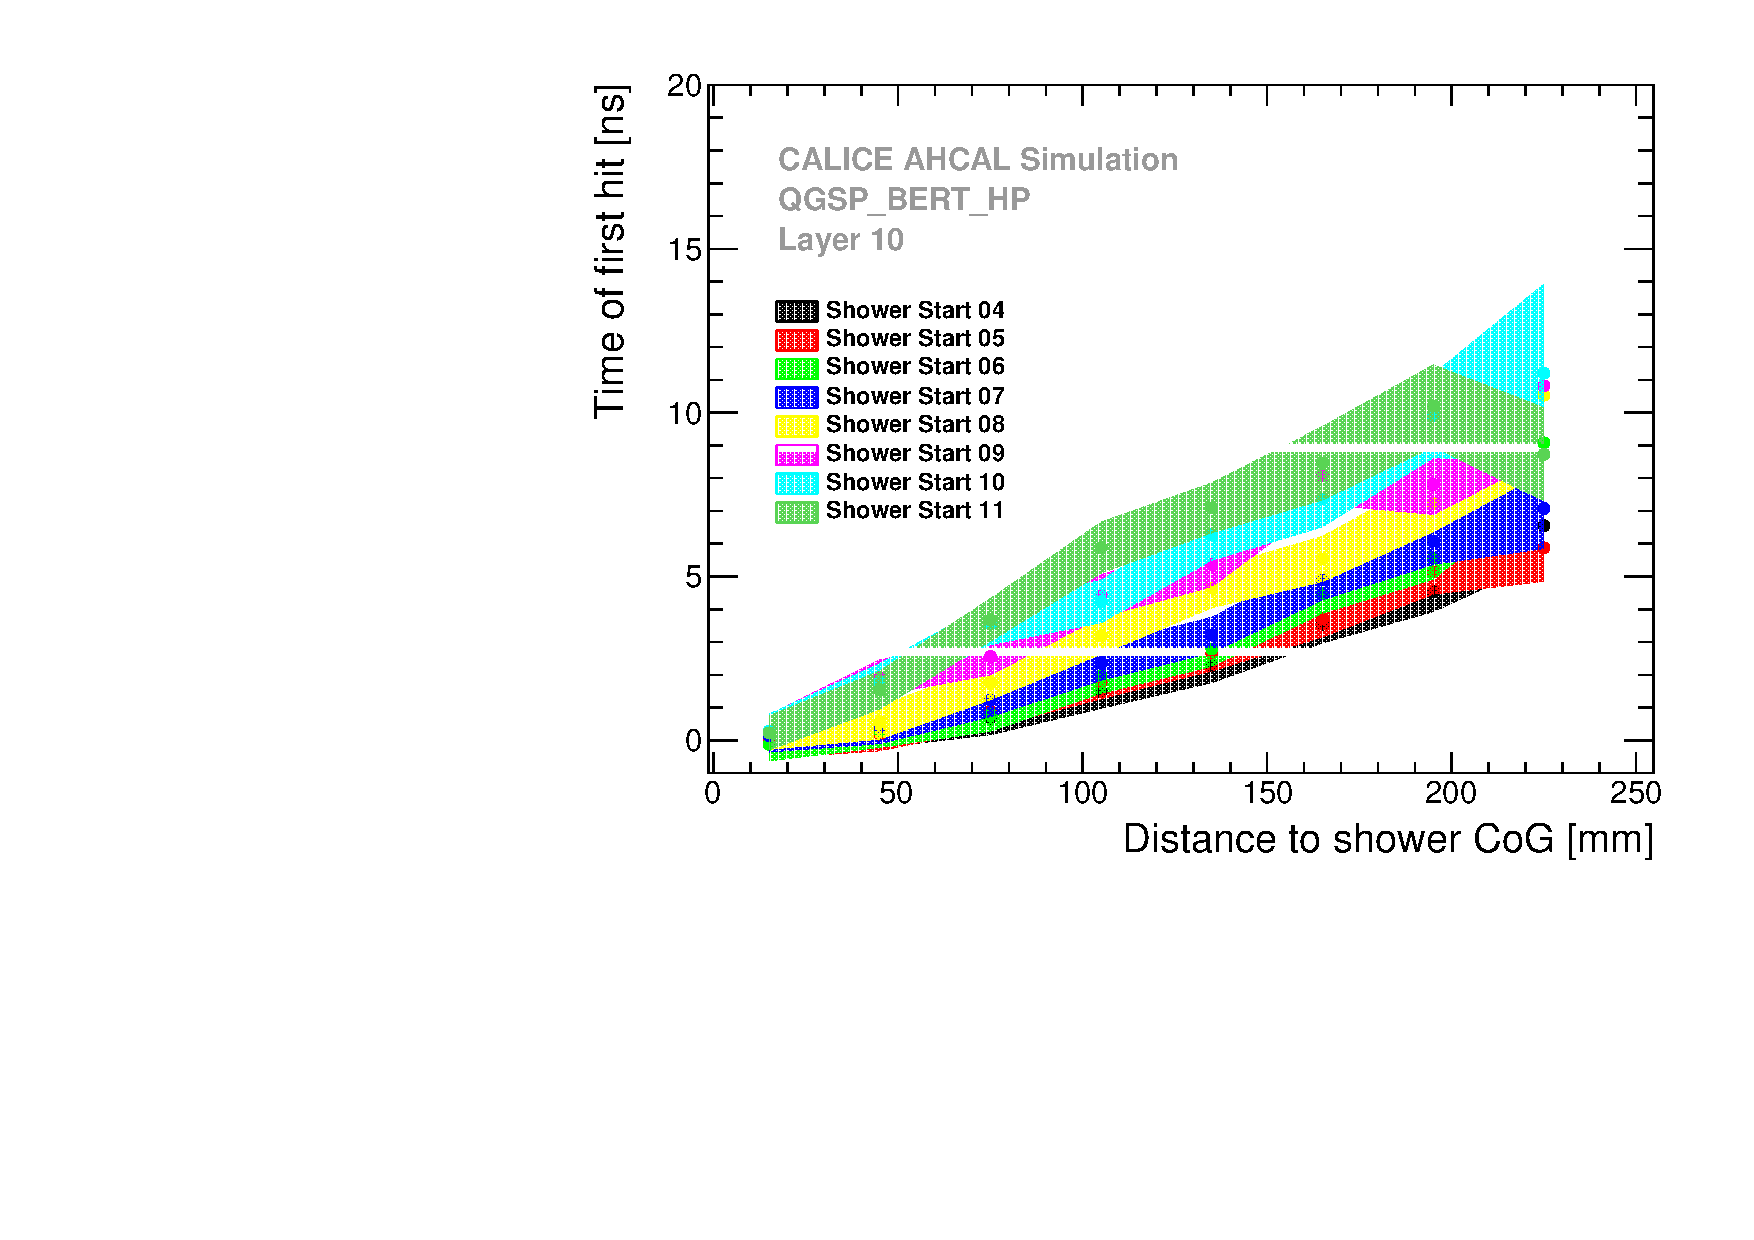
\includegraphics[width=1\textwidth]{../Thesis_Plots/Timing/Pions/Plots/Radius_ShowerStartTruth_FixedModule.pdf}
		\caption{}\label{fig:Radius_FHI_FixedSim}
	\end{subfigure}
	\caption{Mean time of the first hit as a function of the hit distance to the shower axis for 50 GeV pions for different reconstructed FHI layers. In data on the left and in simulation with the QGSP\_BERT\_HP physics list on the right.}
	\label{fig:Radius_FHISim}
\end{figure}

\section{Longitudinal dependence of timing profiles}

Hadronic showers develop as well longitudinally, therefore the longitudinal dependence of mean time of the first hit as a function of the layer position was studied. It is expected that the further you are in the calorimeter that more low energy neutrons contribute to the energy deposition thus enhancing the late tail. The figure \ref{fig:Depth_Comparison} shown the mean time of first hit as function of the layer position for muon, electron and pion beams.

\begin{figure}[htbp!]
	\begin{subfigure}[t]{0.49\textwidth}
		\centering
		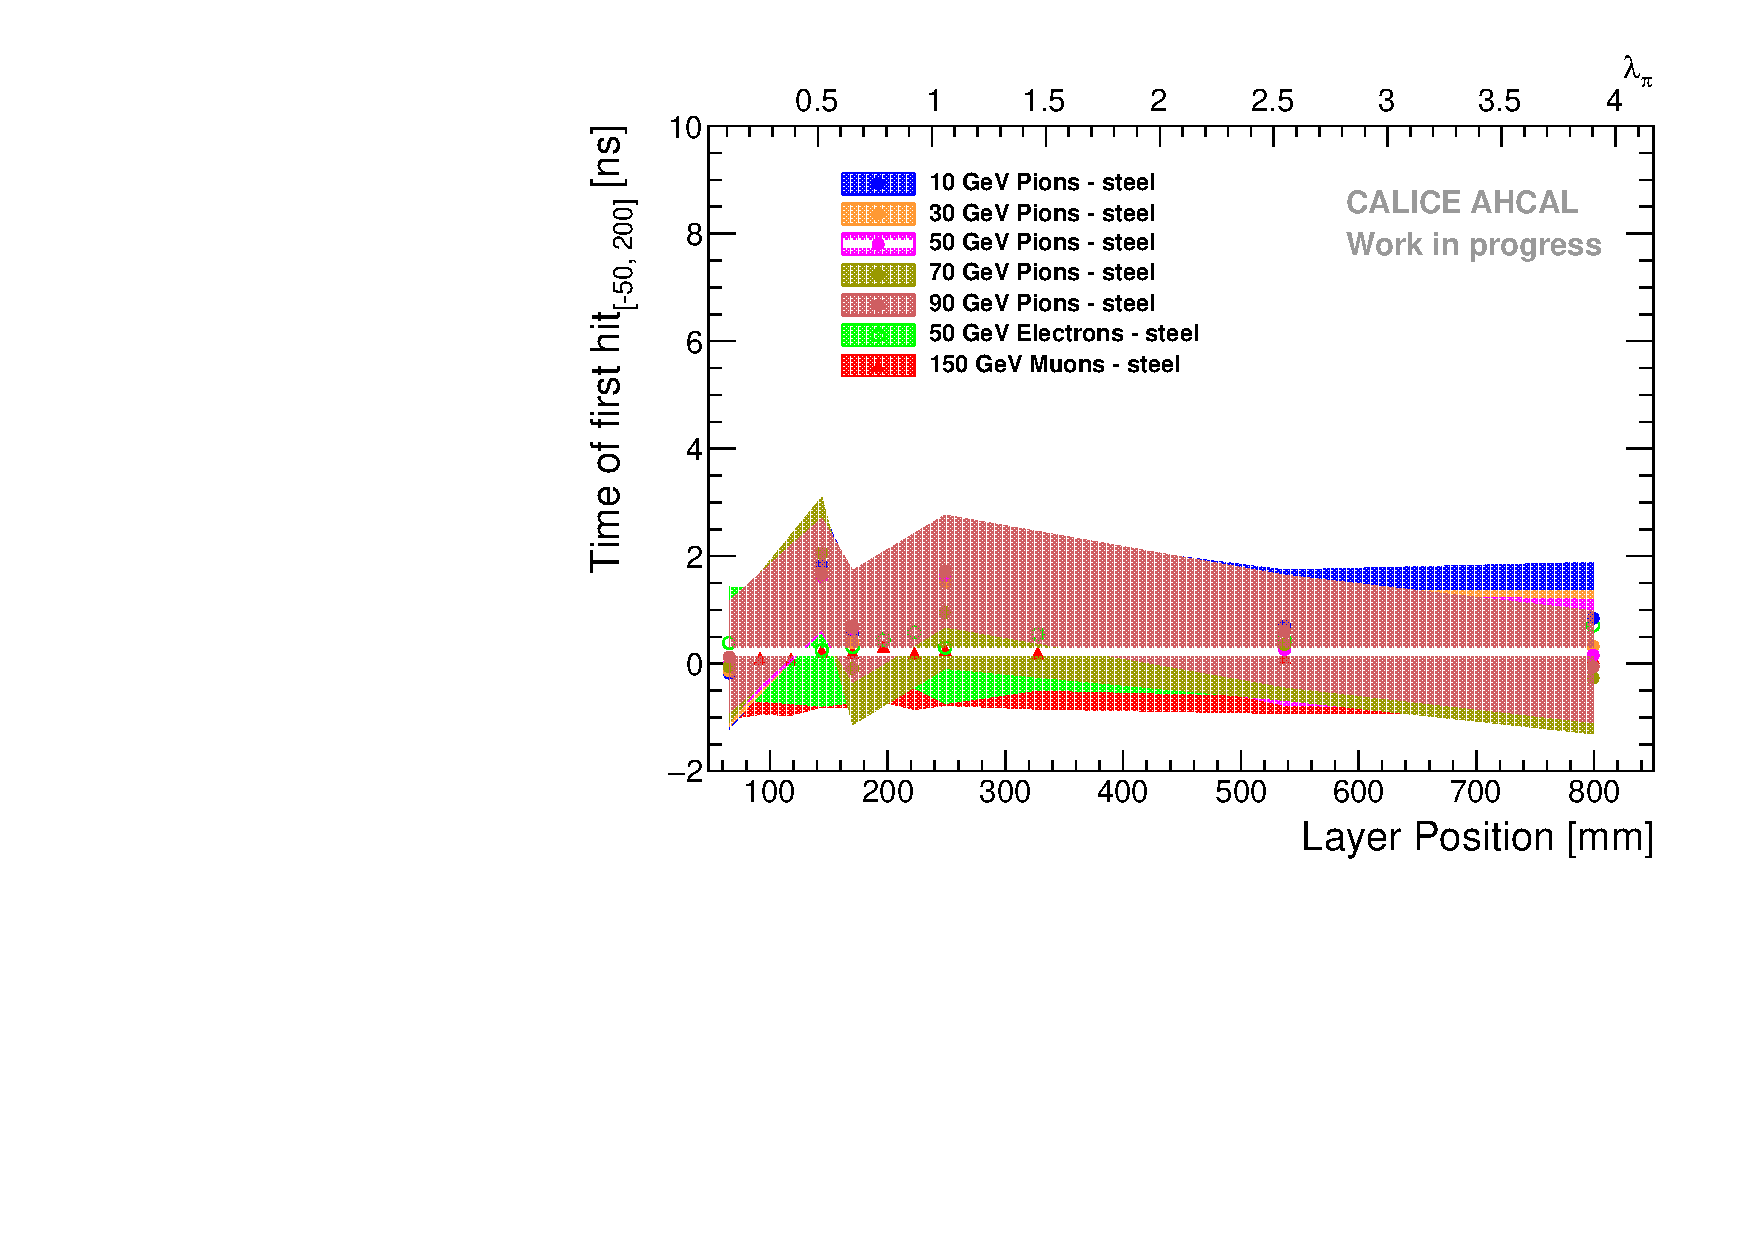
\includegraphics[width=1\textwidth]{../Thesis_Plots/Timing/Pions/Plots/Timing_Depth_Comparison_ShortAsymRange.pdf}
		\caption{} \label{fig:Depth_Comparison}
	\end{subfigure}
	\hfill
	\begin{subfigure}[t]{0.49\textwidth}
		\centering
		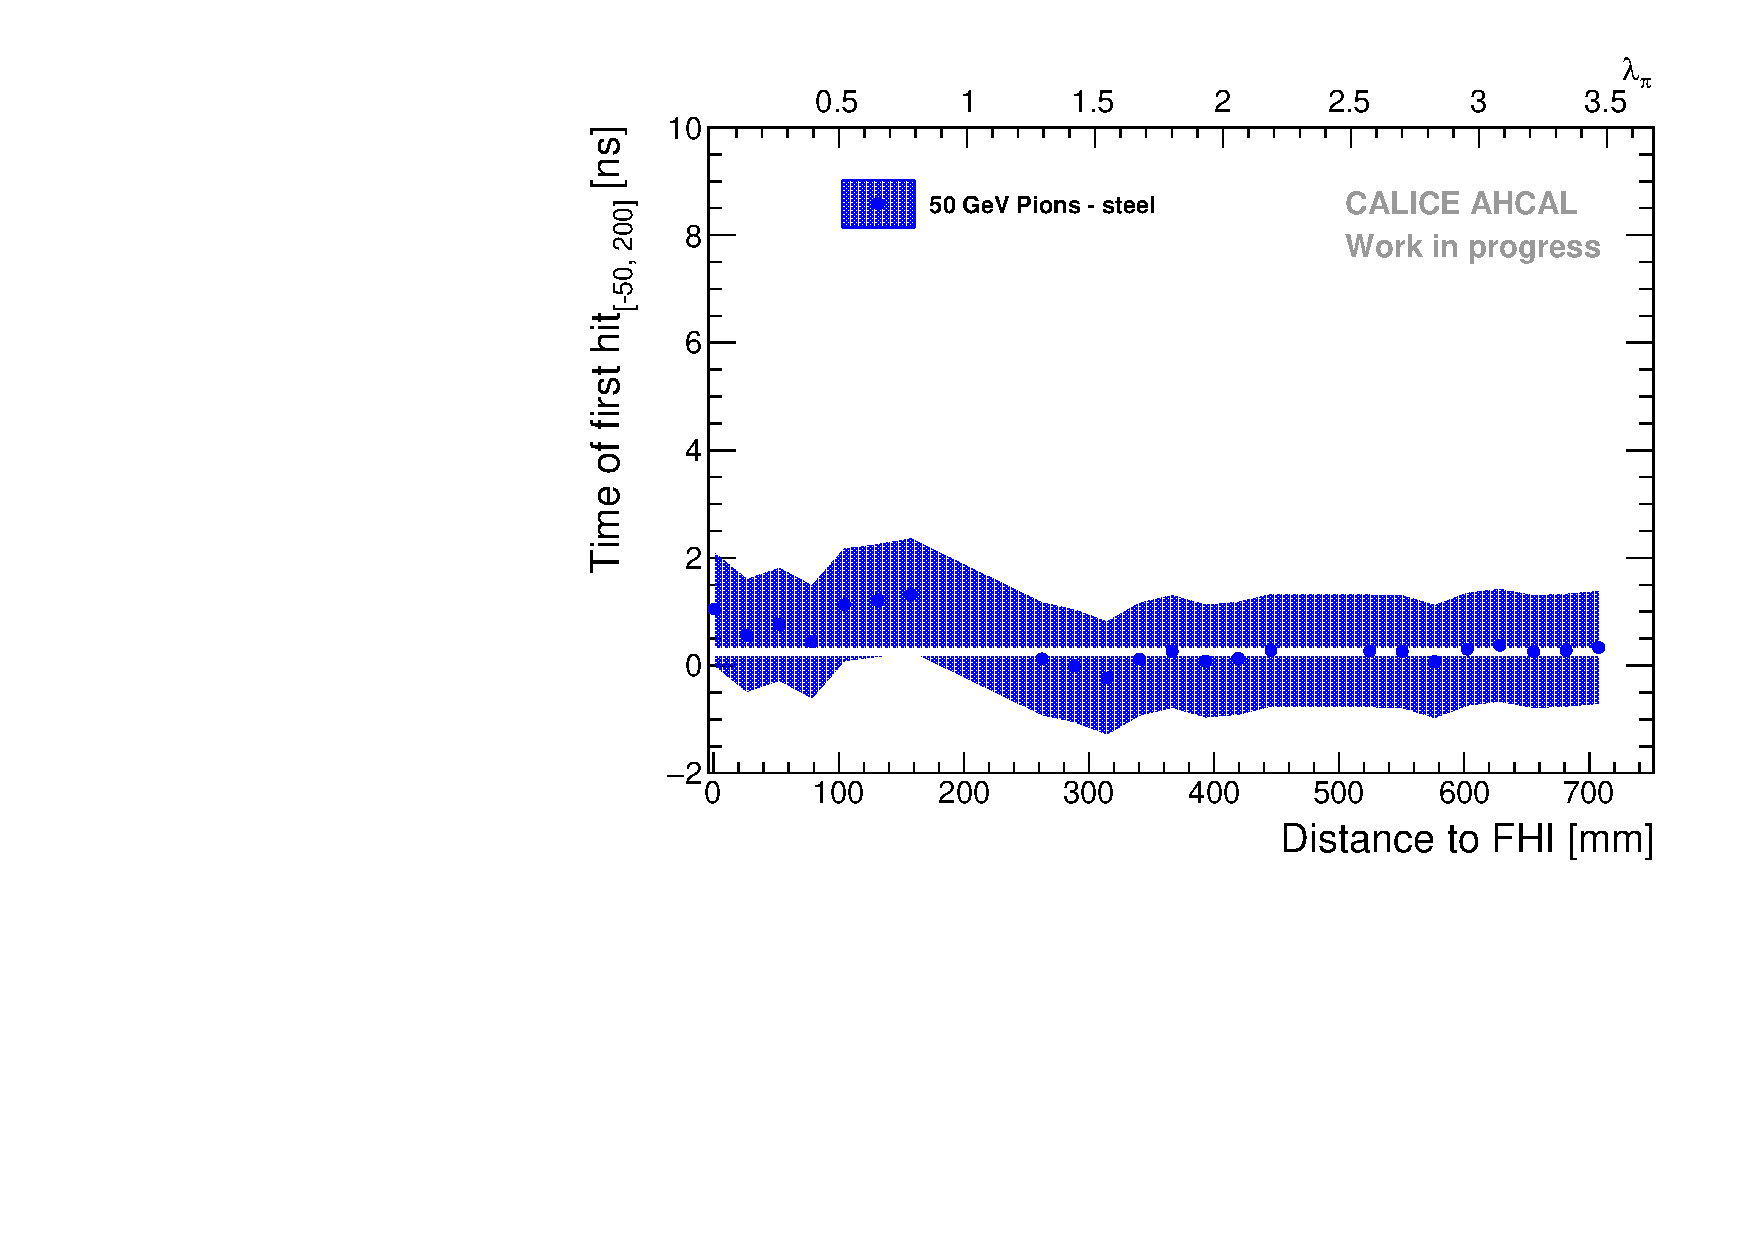
\includegraphics[width=1\textwidth]{../Thesis_Plots/Timing/Pions/Plots/Timing_Depth_Comparison_ShortAsymRange_ShowerStart.pdf}
		\caption{}\label{fig:Depth_Comparison_FHI}
	\end{subfigure}
	\caption{The left plot shows the longitudinal timing profile as a function of the layer position for muon, electron and pion beams. The right plot shows the longitudinal timing profile as a function of the distance to the reconstructed FHI layer for 50 GeV pions.}
	\label{fig:DepthProfile}
\end{figure}

In data, no increase of the mean time is observed as a function of the layer depth and as well no beam energy dependence is visible. This may be due to the late component that is suppressed by the high time resolution of the AHCAL and the systematic uncertainty. An attempt was made to get a better sensitivity by looking at the mean time of first hit as a function of the distance to the reconstructed FHI layer as shown in figure \ref{fig:Depth_Comparison_FHI}. However, the figure still shows a flat distribution centered around 0 ns.

The longitudinal timing profile was also compared to simulations. The mean time of first hit is compatible with a flat distribution around 0 ns for all models. The timing resolution of the AHCAL may be too high in order to be sensitive to any small changes of the mean time over the calorimeter depth. To check this. the simulation with the QGSP\_BERT\_HP physics list without time smearing is shown in figure \ref{fig:Depth_Sim_noSmearing}. It shows that there is an increase of the mean time of first hit as function of the layer in the order of 1 ns and confirms that due to the electronics time resolution this is not visible in data.

\begin{figure}[htbp!]
	\begin{subfigure}[t]{0.49\textwidth}
		\centering
		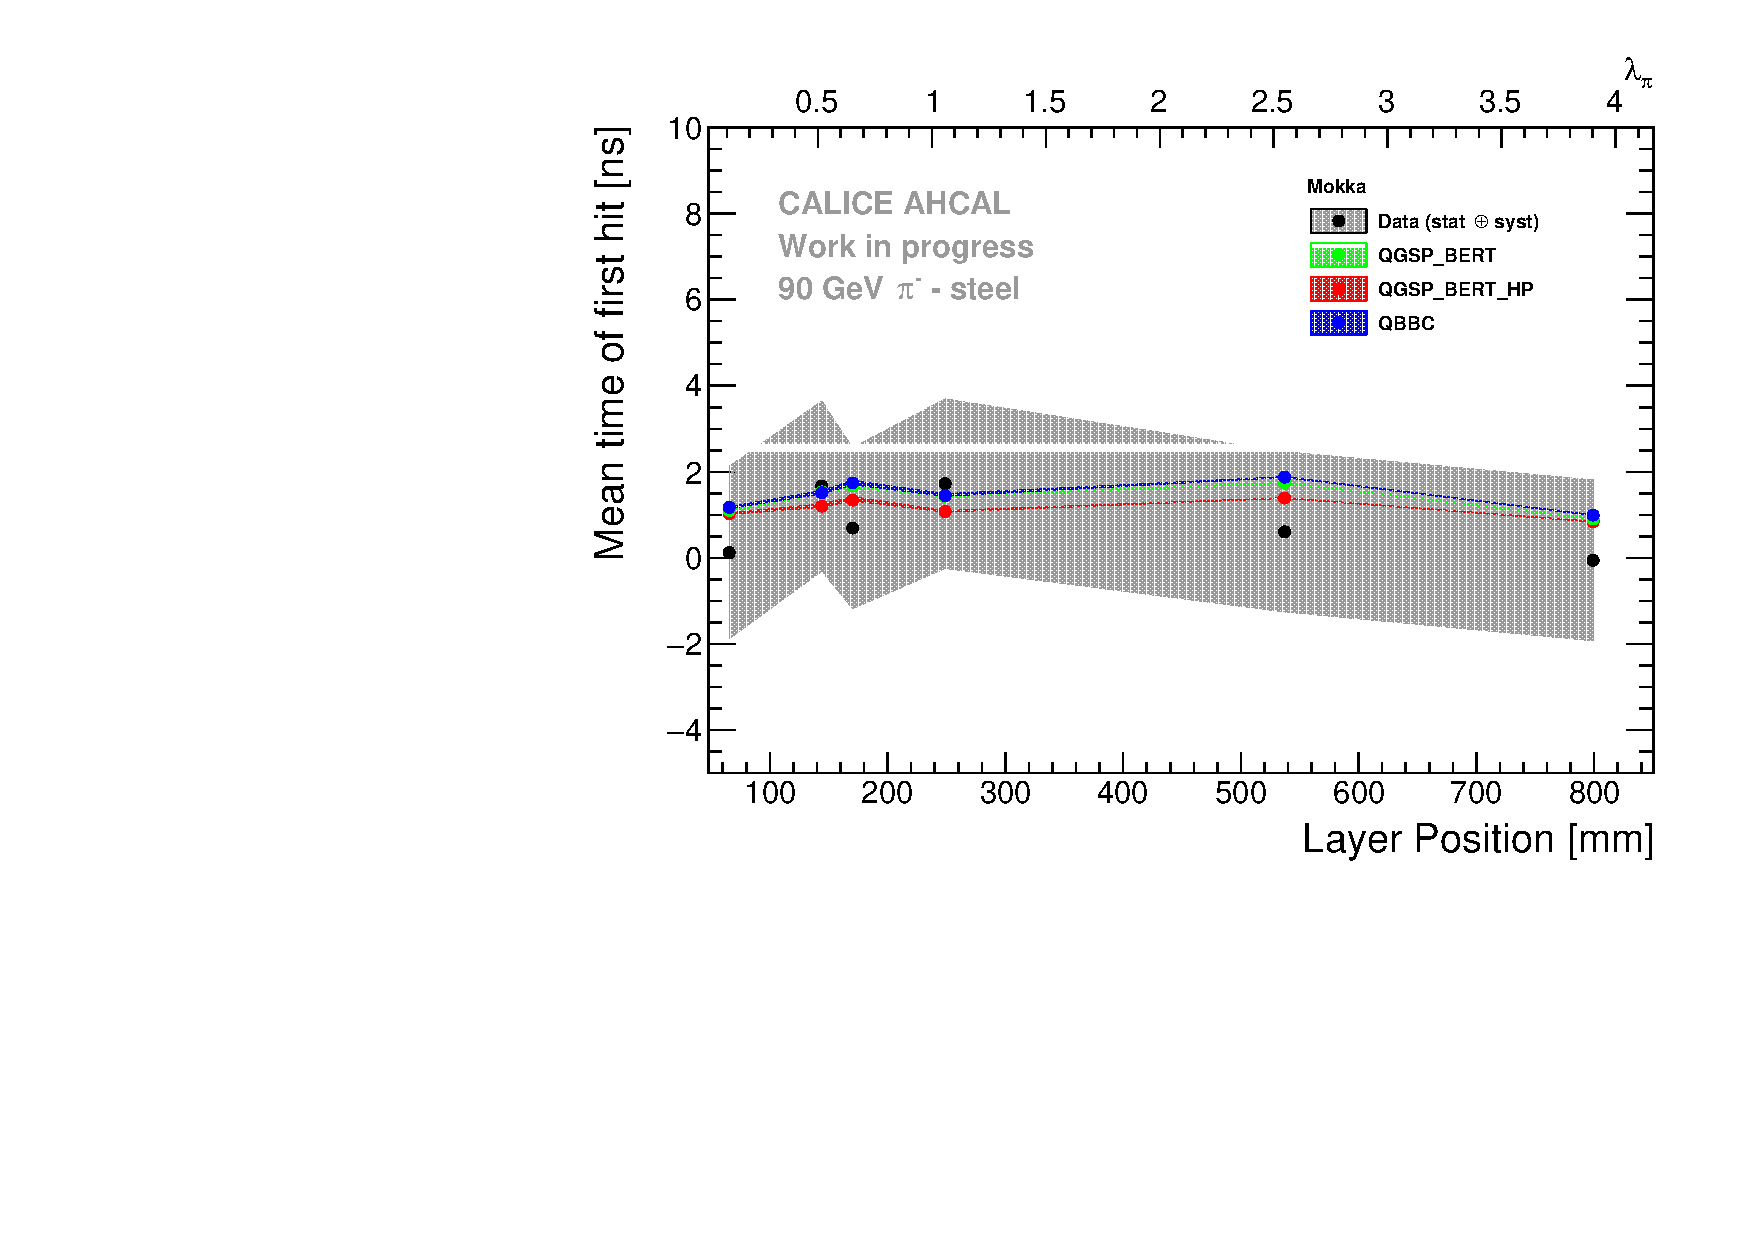
\includegraphics[width=1\textwidth]{../Thesis_Plots/Timing/Pions/Plots/ComparisonToSim/Time_Depth_90GeV_Mokka.pdf}
		\caption{} \label{fig:Depth_SimData_Comparison}
	\end{subfigure}
	\hfill
	\begin{subfigure}[t]{0.49\textwidth}
		\centering
		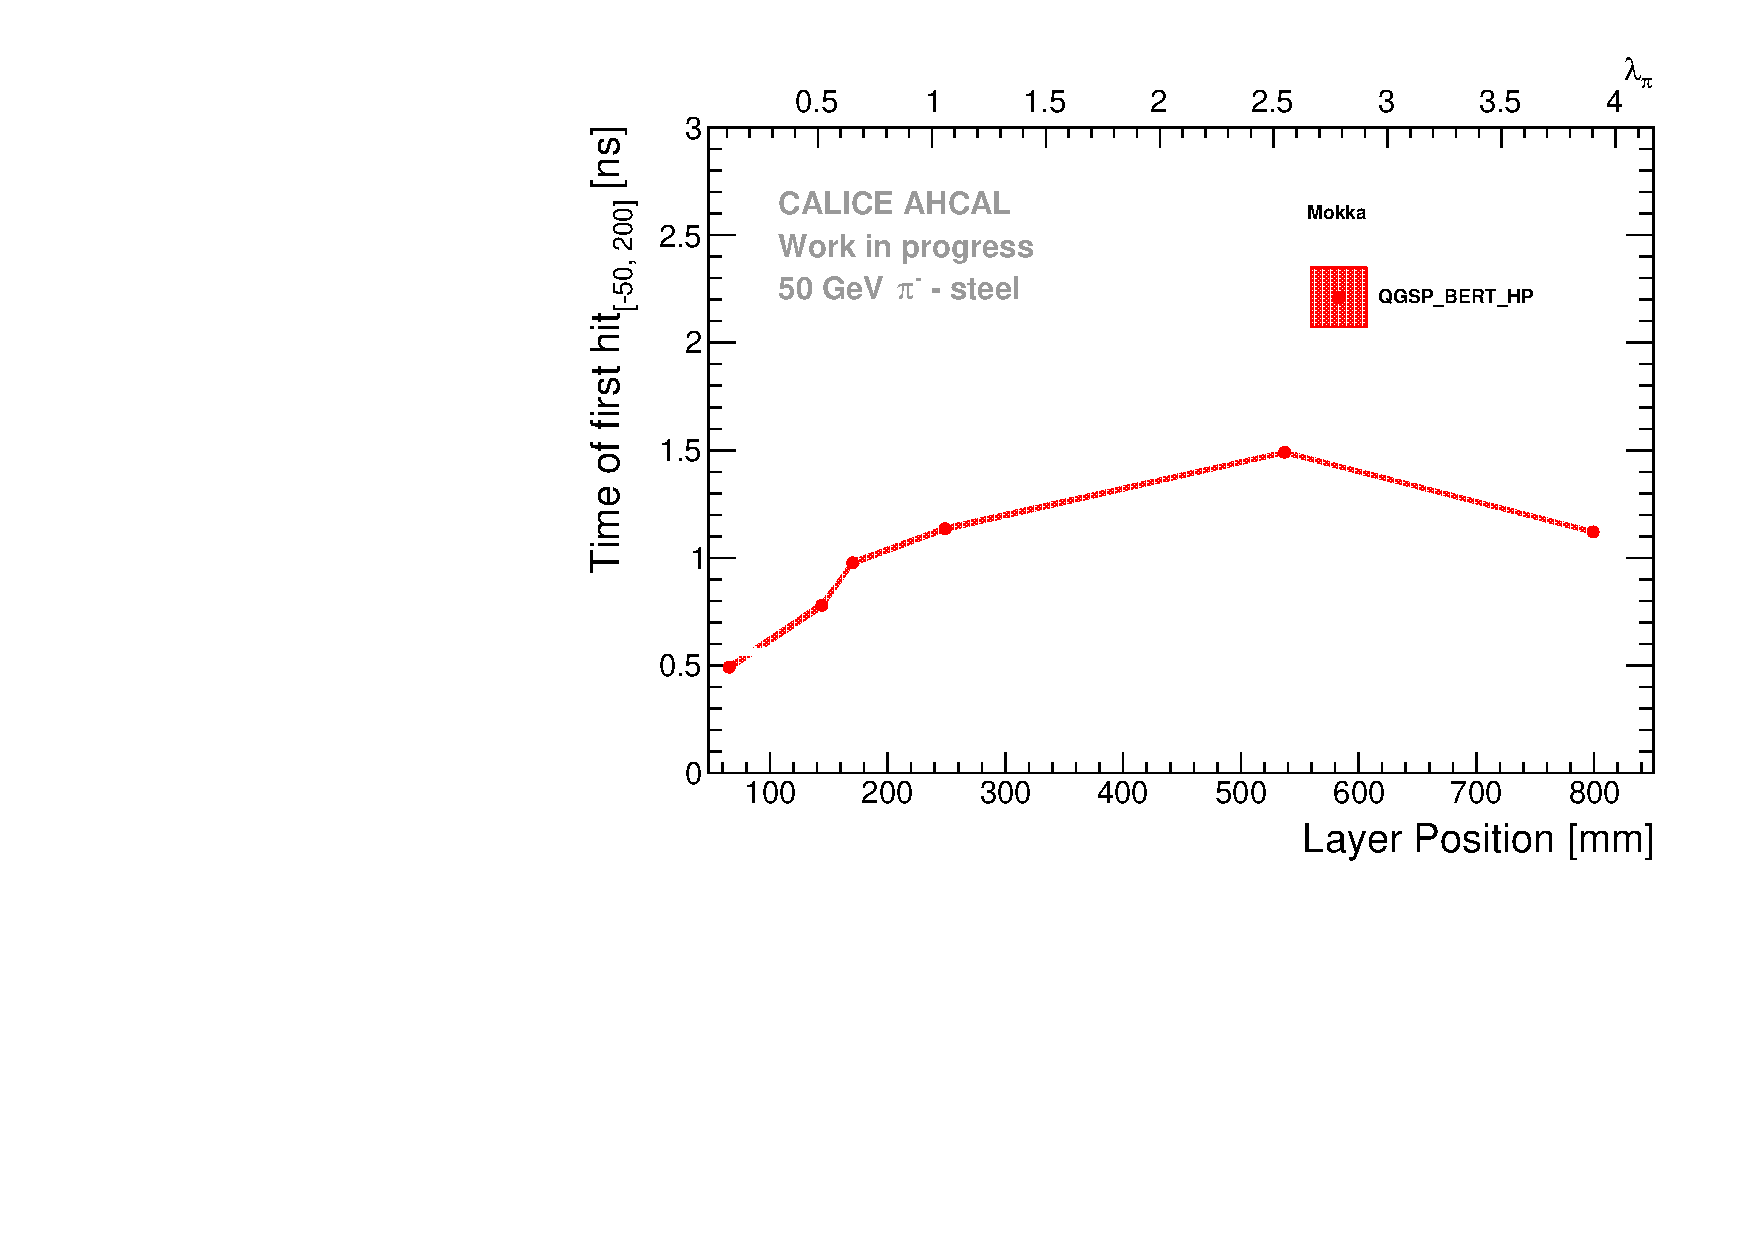
\includegraphics[width=1\textwidth]{../Thesis_Plots/Timing/Pions/Plots/Time_Depth_50GeV_QGSP_BERT_HP_noSmearing.pdf}
		\caption{}\label{fig:Depth_Sim_noSmearing}
	\end{subfigure}
	\caption{On the left, comparison of the time of first hit as a function of the layer position in data and \mokka simulation for 90 GeV pions. The grey and color bands shows the systematics. On the right, time of first hit as function of the layer position for 50 GeV pions in simulation with the QGSP\_BERT\_HP physics list with no time smearing.}
\end{figure}

\section{Time correlations between layers}

The advantage of this studied prototype over T3B is the possibility to investigate time correlations between layers. For this study, the data below 50 ns is ignored as only the tail of the timing distributions is interesting.

The procedure is done by looking at each hit in layer $i$ and checking in layer $i+1$ for a hit within a distance of 60 mm in the $x:y$ plane. If a hit is found, both times are plotted against each other. If more than one hit is found in layer $i+1$ within a radial distance of 60 mm, the closest in the $x:y$ plane is taken.

Two types of correlations were investigated, short and long. For the short correlation, the layers 6 and 7 were chosen, corresponding to 1 $X_0$ or 0.1 $\lambda_{\pi}$. As for the long, the layers 13 and 14 were selected, corresponding to 10 $X_0$ or 1 $\lambda_{\pi}$. These were chosen due to the fact that few layers were working properly. It is expected that EM sub-showers can lead to a correlation of hit times for the layers 6 and 7, while the layers 13 and 14 are far apart, and therefore would show less correlation of hit times. The hit times correlation is shown in figure \ref{fig:TimeCorrelation} for the 50 GeV dataset.

The figures show that a correlation is visible in the data for both cases. To quantify this, the following ratio is calculated
\begin{equation}\label{eq:CorrelCalcul}
	R = \frac{\int_{50 ns}^{2 \mu s} \int_{50 ns}^{2 \mu s} \frac{dN_i(t)}{dt_i} \frac{dN_j(t)}{dt_j} dt_i dt_j}{N_{tot}}
\end{equation}
where N$_{tot}$ is the total number of entries in the histogram and the nominator is the number of entries between 50 ns and \SI{2}{\micro\second} in the red box of the above figures.

The results show that 18.19\% of the entries are in the red box region for the short correlation. This may come from EM sub-showers in the hadron shower. For the long correlation, 3.24\% of the entries are in the red box region. This represents a substantial amount of hits that are correlated.

\begin{figure}[htbp!]
	\begin{subfigure}[t]{0.49\textwidth}
		\centering
		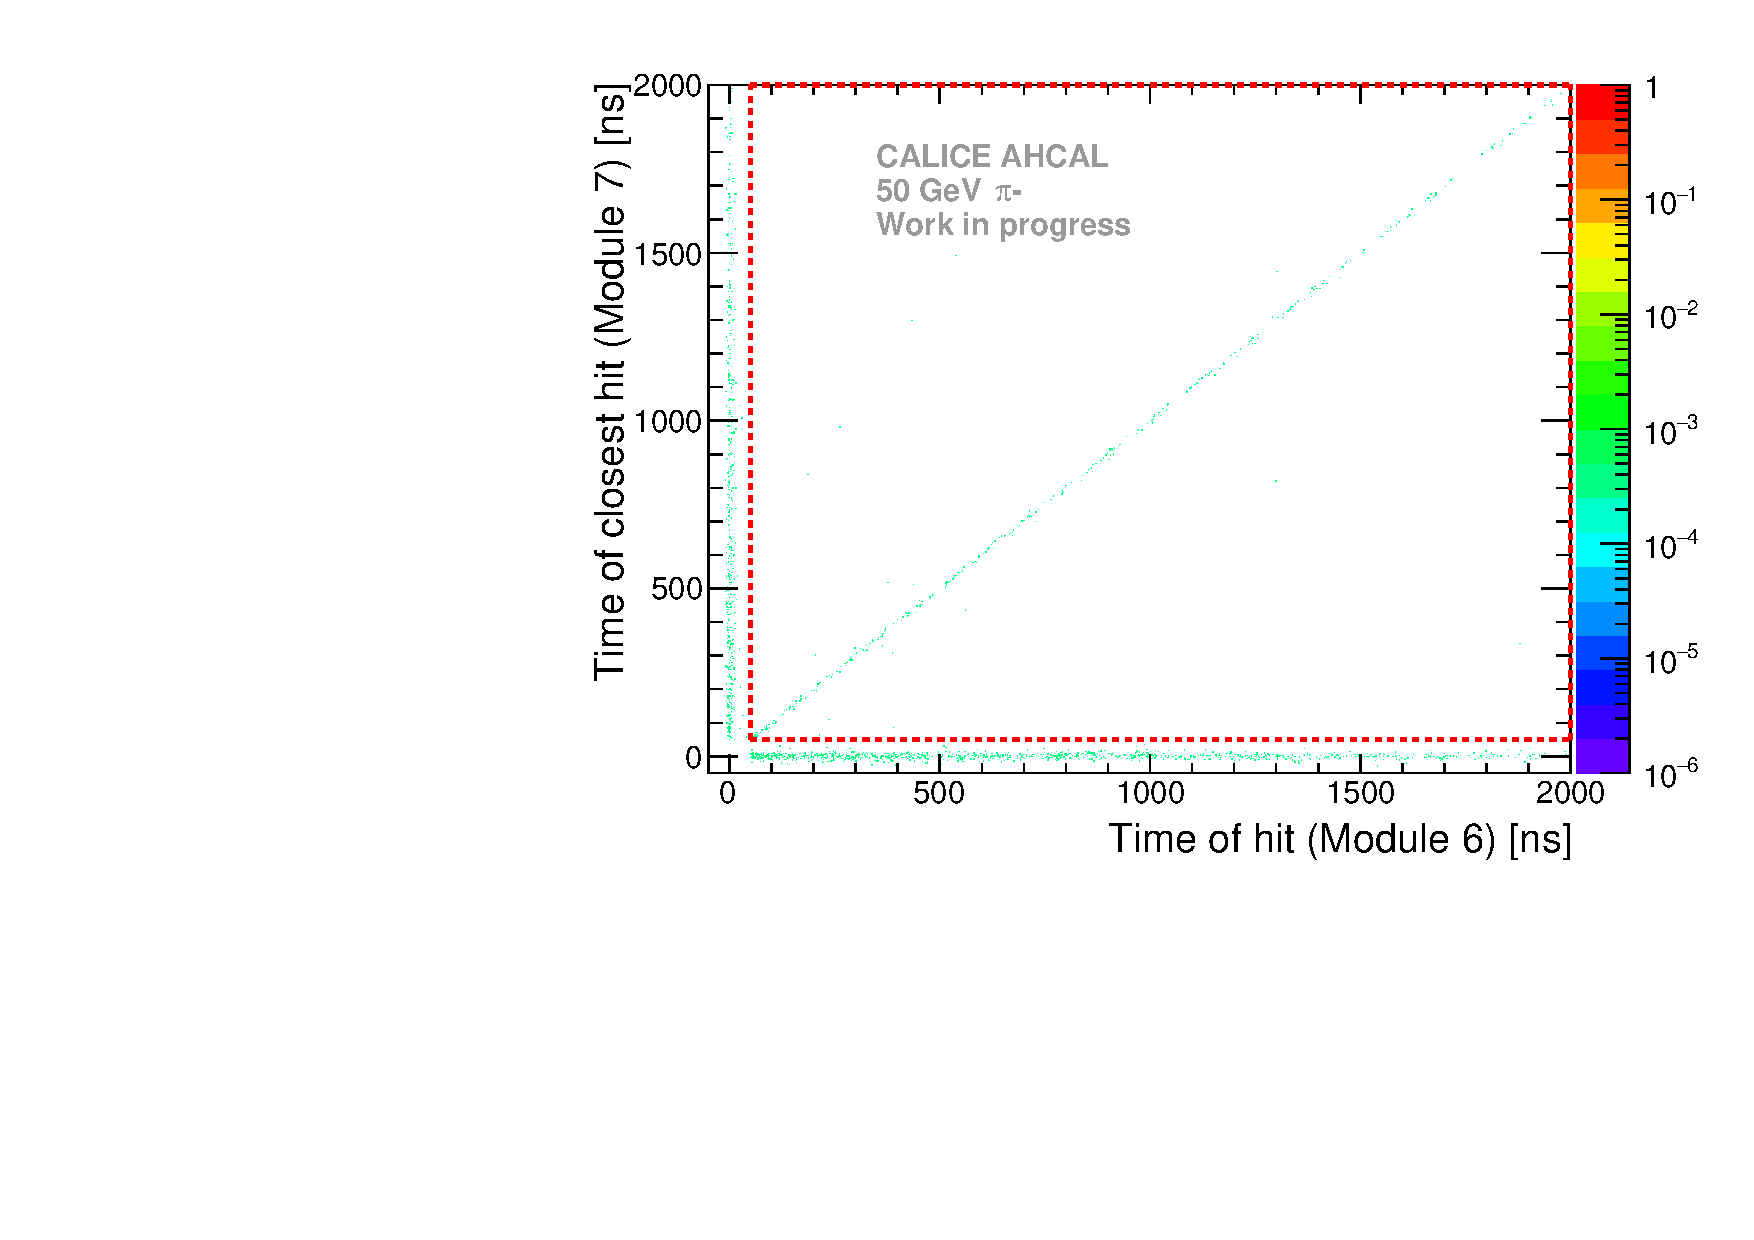
\includegraphics[width=1\textwidth]{../Thesis_Plots/Timing/Pions/Plots/Time_Correlation_short.pdf}
		\caption{} \label{fig:Time_Corr_short}
	\end{subfigure}
	\hfill
	\begin{subfigure}[t]{0.49\textwidth}
		\centering
		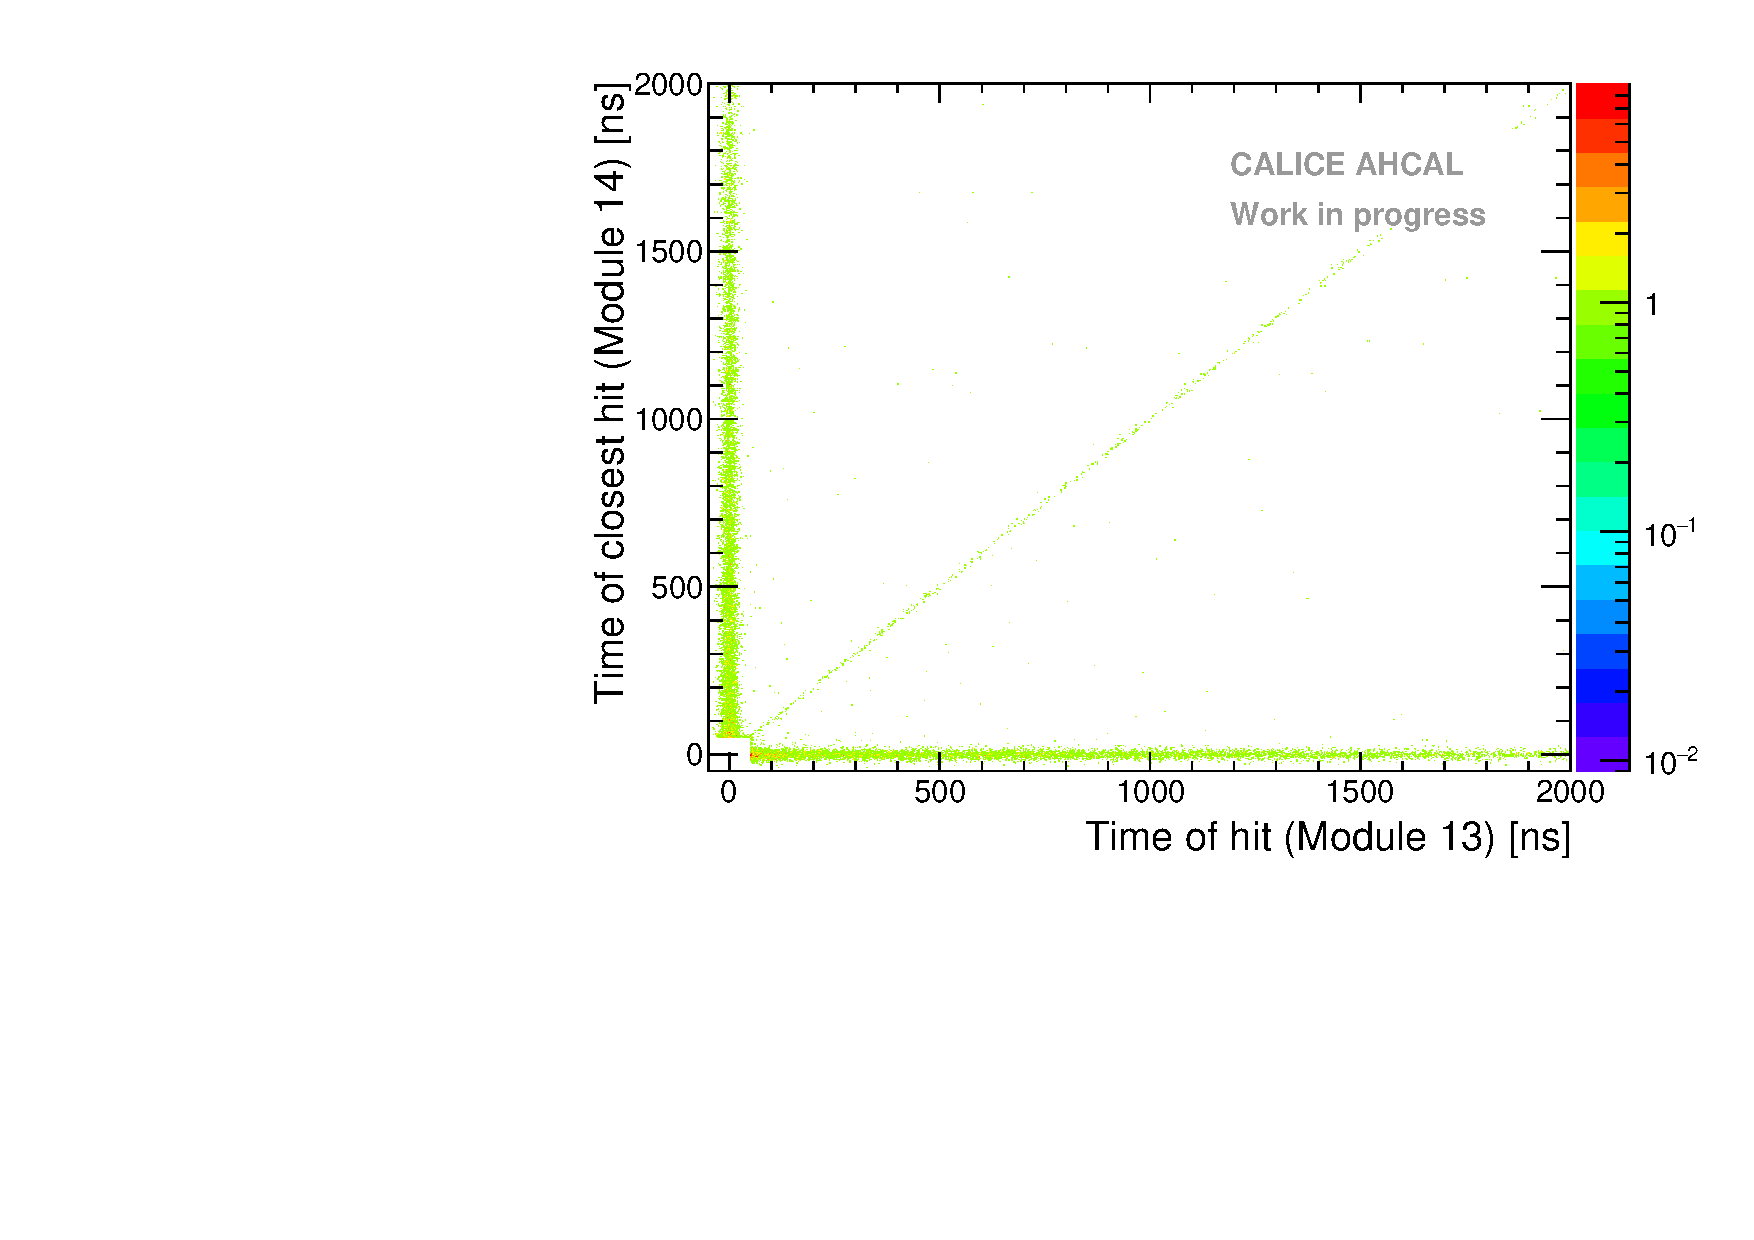
\includegraphics[width=1\textwidth]{../Thesis_Plots/Timing/Pions/Plots/Time_Correlation_long.pdf}
		\caption{}\label{fig:Time_Corr_long}
	\end{subfigure}
	\caption{The left plot shows the time correlation between layer 6 and 7 separated by 1 $X_0$. The right plot shows the time correlation for layers 13 and 14 separated by 1 $\lambda_{\pi}$. Each bin is normalized to the number of entries in the 2D histogram. The red box represent the region of interest. Both plots show a visible time correlation.}
	\label{fig:TimeCorrelation}
\end{figure}
\begin{figure}[htbp!]
	\begin{subfigure}[t]{0.49\textwidth}
		\centering
		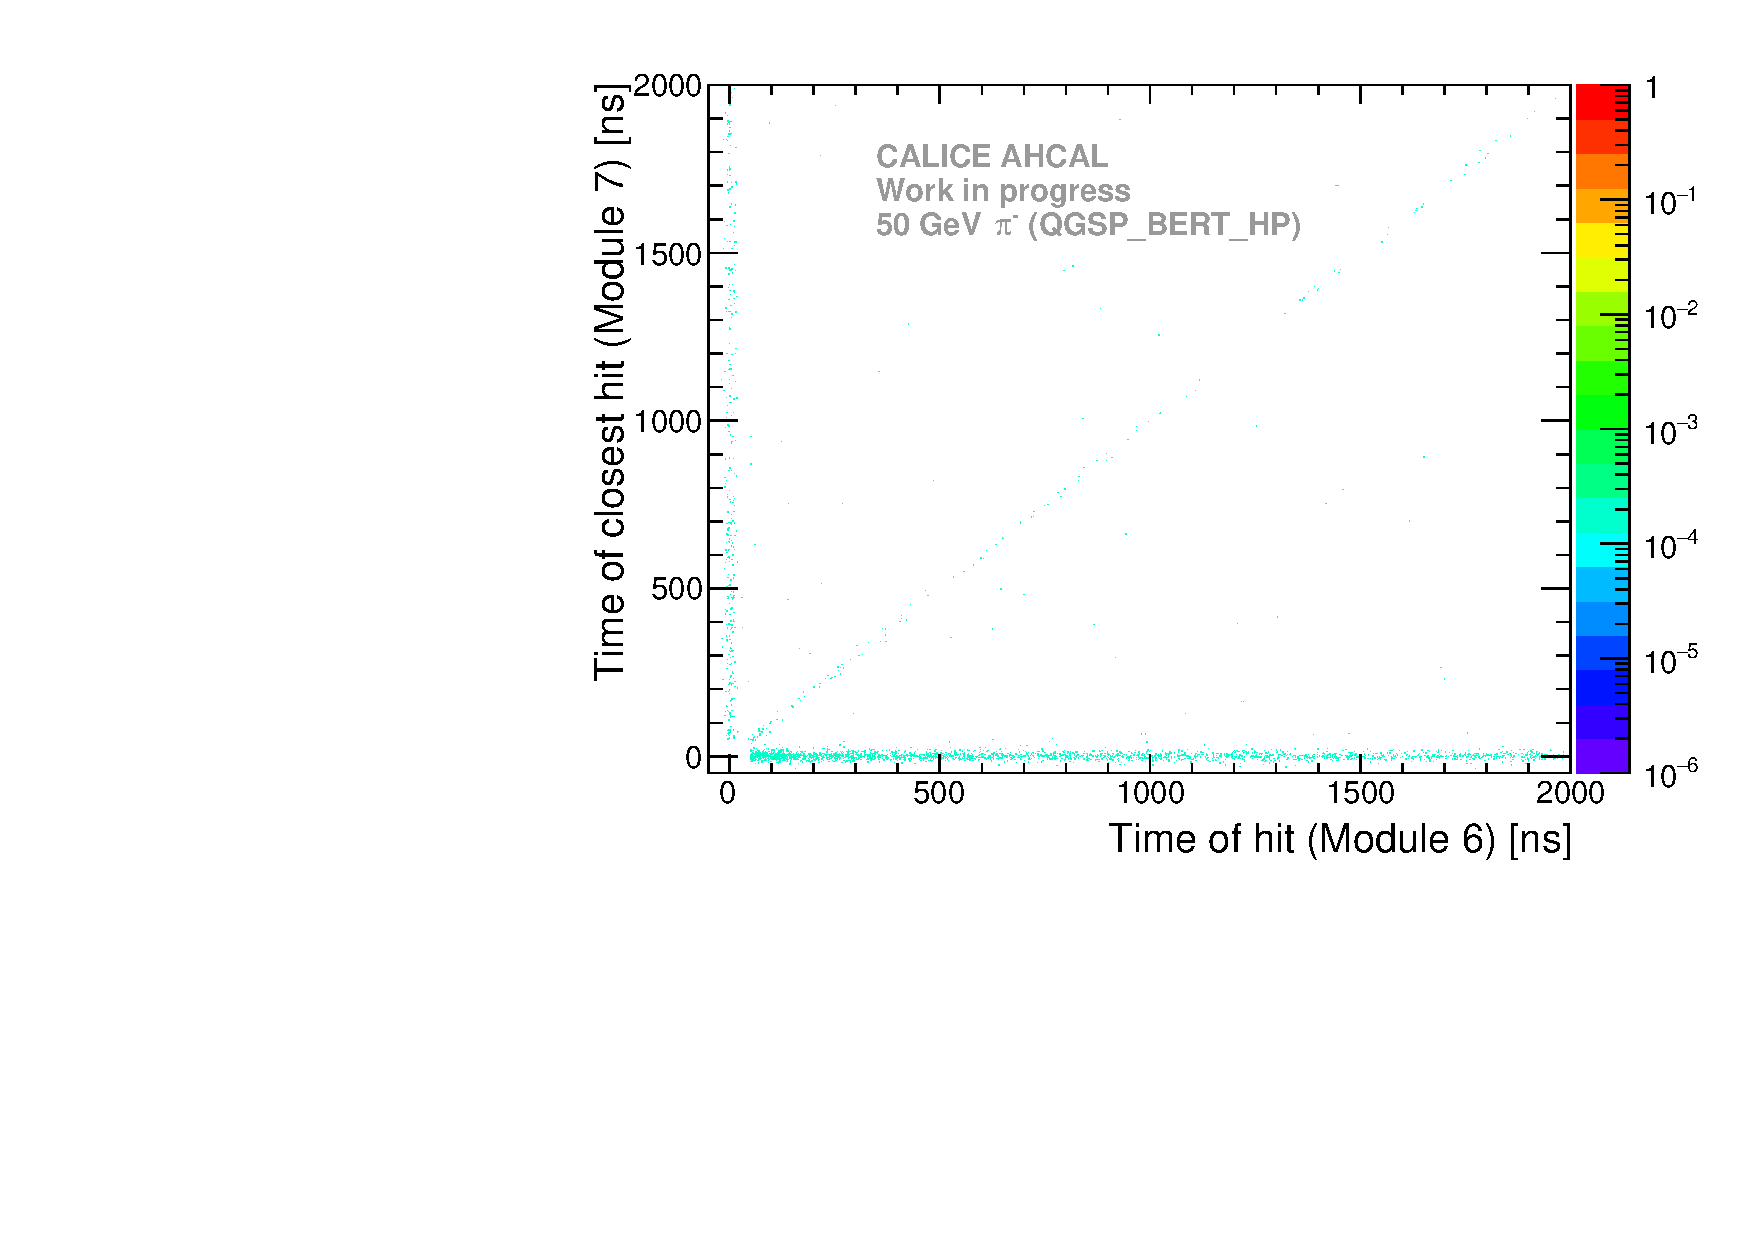
\includegraphics[width=1\textwidth]{../Thesis_Plots/Timing/Pions/Plots/ComparisonToSim/Time_Correlation_50GeV_short_QGSPBERTHP.pdf}
		\caption{Short correlation (QGSP\_BERT\_HP).} \label{fig:Corr_short_QGSPBERTHP}
	\end{subfigure}
	\hfill
	\begin{subfigure}[t]{0.49\textwidth}
		\centering
		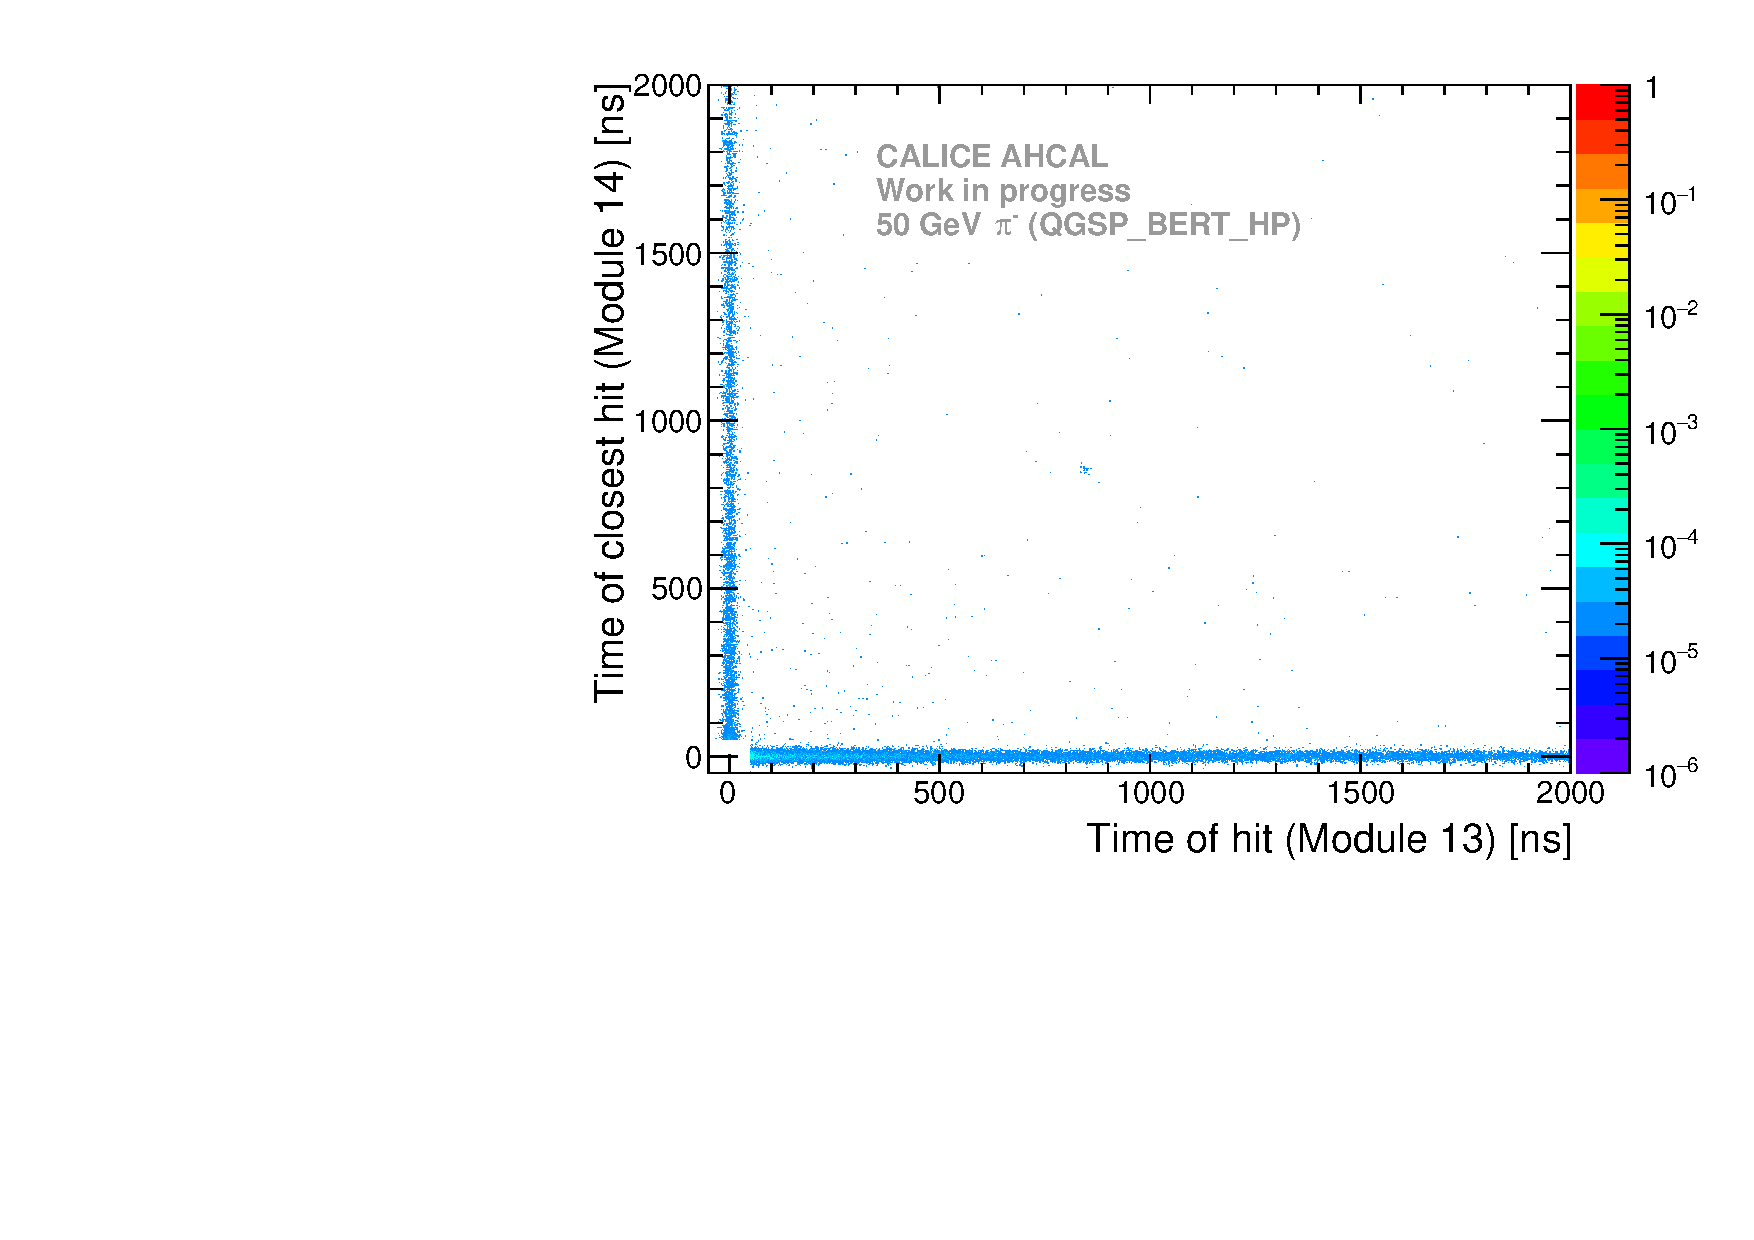
\includegraphics[width=1\textwidth]{../Thesis_Plots/Timing/Pions/Plots/ComparisonToSim/Time_Correlation_50GeV_long_QGSPBERTHP.pdf}
		\caption{Long correlation (QGSP\_BERT\_HP).} \label{fig:Corr_long_QGSPBERTHP}
	\end{subfigure}
	\caption{Hit timing correlations between layers 6 and 7 and layers 13 and 14 in the \mokka simulation with QGSP\_BERT\_HP for 50 GeV pions. Each bin is normalized to the total number of entries in the 2D histogram.}
	\label{fig:Corr_Mokka_Simulation}
\end{figure}

This was compared to simulation using the QGSP\_BERT\_HP physics lists as shown in figures \ref{fig:Corr_Mokka_Simulation}. The figures for simulations with other physics lists can be seen in appendix \ref{appendix:TimingAdd}. In the same way, the number of correlated time hits was calculated and it is summarized in table \ref{table:Correlation_DataSim}. In general, the simulation possesses less correlated hits than in data for both type of correlations. In addition, the choice of the physics list is irrelevant for this observable as all physics lists give the same result within 0.1\% maximum. Furthermore, the \ddhep simulation has slightly less correlated hits, around 1\%, at a short range than in the \mokka simulation which is not understood but it is still within statistical uncertainties.

Comparing data and simulations, there is a large discrepancy for the short range correlation with a difference of around 15\%. For the long correlation, the numbers also differ by around 3\% but it is still within uncertainties. The reason for the discrepancy between data and simulation is not clear though it may come from the selection of the data that may be not good enough to reject multi-particle events as shown figure \ref{fig:DoubleParticleEvent}, therefore providing more correlated hits than observed in simulation. More data, especially with a better detector to be sure to reject multi-particle events, is required in order to understand the origin of such correlations.

\begin{table}[htb!]
	\centering
	\caption{Table with fraction of events in the red box region as calculated with equation \ref{eq:CorrelCalcul}. The top is for \mokka simulations, the bottom is for \ddhep simulations. The quoted errors are only statistical errors.}
	\label{table:Correlation_DataSim}
	\begin{tabular}{@{} lcc @{}}
		\toprule
		Type & Short correlation [\%] & Long correlation [\%]\\
		\midrule
		\multirow{2}{*}{Data} & \multirow{2}{*}{18.19 $\pm$ 5.13} & \multirow{2}{*}{3.24 $\pm$ 3.79}\\ & &\\
		\midrule
		\multirow{2}{*}{QGSP\_BERT} & 4.08 $\pm$ 3.44 & 0.65 $\pm$ 2.65\\ & 3.01 $\pm$ 4.72 & 0.68 $\pm$ 3.25\\
		\multirow{2}{*}{QGSP\_BERT\_HP} & 4.1 $\pm$ 3.44 & 0.67 $\pm$ 2.65\\ & 3.06 $\pm$ 4.72 & 0.71 $\pm$ 3.25\\
		\multirow{2}{*}{QBBC} & 4.09 $\pm$ 3.44 & 0.66 $\pm$ 2.65\\ & 3.02 $\pm$ 4.72 & 0.69 $\pm$ 3.25\\
		\bottomrule
	\end{tabular}
\end{table}

\section{Summary and Outlook}

The understanding of the time structure of hadronic showers and the level of accuracy reflected in \geant simulations is highly relevant for calorimeters at future (linear) collider experiments. This can be applied for conditions with a high level of background such as $\gamma\gamma \rightarrow \text{hadrons}$ or high repetition rates experiments to remove out-of-time pile-up events.

A testbeam at the SPS facility at CERN in July 2015 was focused to enhance the knowledge of the time development of hadronic showers. The AHCAL technological prototype, close to the ILD detector design, was equipped with 14 layers inserted in a steel absorber and using scintillator tiles as active material readout by SiPMs to provide radial and longitudinal sampling of showers with a high granularity and a ns-scale time resolution. For the first time, time study of hadronic showers was done which such granular calorimeters using integrated readout electronics.\\[0.1cm]

\noindent\textbf{Energy scale calibration:} In chapter \ref{chap:ECalibAHCAL}, the energy scale calibration of the AHCAL was presented. 85\% of the AHCAL detector channels have been calibrated to a precision of around 1.7\%. The validation studies of the simulation concluded that the a good average energy calibration is achieved at the cell level. In addition, the simulation has been further validated with electromagnetic showers and it showed that the data is well reproduced at a level of 10-20\% precision.\\[0.1cm]

\noindent\textbf{Time calibration of the AHCAL:} In chapter \ref{chap:TimingCalib}, the time calibration procedure of the AHCAL was presented. More than 20000 constants have been determined from data. A time resolution of 5.65 ns is achieved after a simple time calibration of the AHCAL. However, several effects from the front-end electronics can be corrected. The non-linearity correction ,related to the non-linearity of the TDC ramp in the ASIC, improves the time resolution by around 5\% and the time-walk correction, related to the slow shaper in the ASIC that delays low amplitude signals, improves the time resolution further by 3\%. At the end, a time resolution of the order of 5 ns is achieved for minimum ionizing particles.\\[0.1cm]

\noindent\textbf{Validation of the time calibration:} In chapter \ref{chap:TimingValidation}, the timing calibration was cross-checked with the electron dataset recorded at CERN and the timing simulation has been validated. It was expected that a time resolution in the same order of magnitude or better than the time resolution obtained for MIPs would be achieved. However, due to the readout electronics that affects the time resolution as a function of the number of triggered channels in a chip, the time resolution for electron is worse with a value between 7.5 to 8.2 ns for beam energies between 10 and 50 GeV. This effect has been parametrized from data and implemented in the time smearing for the simulation. The simulation reproduces the data within 10-20\% for all electron beam energies. However, the tails of the time distribution are not well reproduced due an imperfect implementation of noise hits. Nevertheless, this is considered good enough for looking at the time development of pion showers.\\[0.1cm]

\noindent\textbf{Timing of hadron showers:} In chapter \ref{chap:TimingPions}, the timing of hadronic showers was studied. Firstly, the absolute time of first hit distribution has been investigated. The data shows a clear tail to late hits compared to MIP and electron time distributions. A comparison with simulation has been done for pion beam energies between 10 GeV and 90 GeV. The comparison showed that the QGSP\_BERT\_HP and QBBC physics lists agree well with the data. However, the QGSP\_BERT physics list overestimate the amount of hits in the late tail by around a factor 10. Secondly, the energy dependence of the hit time has been studied. The data shows that late hits are concentrated at low hit energies below 1 MIP in iron. The comparison with simulation showed that for 10 GeV pions, the simulation agrees well with the data within the systematics uncertainty. However, for higher pion beam energies, a difference is visible at low hit energies between 0.5 MIP and 1.5 MIP where the simulation lies above the data. The difference seen may be due to the time correction of the data as a function of the number of triggered channels that is not perfect. For hit energies above 3 MIP, the data and simulation are in agreement. Thirdly, the radial dependence of the hit time has been investigated. This dependence has been looked at separately for layers 3 to 10 (single HBU) and layers 11 to 14 (2 by 2 HBU) due to a decrease of the mean hit time at the transition radius between the two type of layers. This has been studied in more details and concluded that this feature may be due to a dependence as a function of the start of the shower that showed that the radial dependence of the mean time of first hit decreases with deeper layers. The simulation reflects this feature as well. Anyhow, the data shows that late hits are mostly at a great distance from the shower axis, while prompt hits from electromagnetic sub-showers and relativistic hadrons are predominant near the shower axis. A comparison between data and simulation has been carried out and showed that the QGSP\_BERT\_HP physics list agrees well with the data but the QBBC and QGSP\_BERT physics lists agree with the data up to a hit distance to the shower axis of 100-150 mm and for higher hit distances to the shower axis, these physics lists tend to overestimate the late depositions by 1-3 ns. Fourthly, the longitudinal dependence of the hit time has been studied. This study concluded that there are no visible dependence for all beam energies. This is due to the timing resolution of the AHCAL that is too high. The simulation without time smearing shows that an increase of the mean time of around 1-1.5 ns is visible as a function of the layer depth. Finally, timing correlations between layers have been investigated. Short range (1 $X_0$ separation) and long range (10 $X_0$ or 1 $\lambda$ separation) have been looked at. Time correlations are visible at short range as well as long range in different proportions in the data. In addition, a comparison of detailed simulations with data has been performed. It shows that in general, time correlations are reproduced in simulation but the amount of hits in data and simulation differ quite significantly. This may be due to the selection of the data that does not reject efficiently multi-particle events. More data and investigations to understand the origin such time correlations are needed.\\[0.1cm]

Furthermore, the time resolution achieved in testbeam does not reflect the time resolution that could be accessible in an ILC running mode due to a different frequency of the slow clock (250 kHz in testbeam compared to 5 MHz at the ILC). By extrapolation, assuming that the time resolution scales linearly with the frequency of the slow clock, a time resolution of the order of 1 ns could be obtained in an ILC running scenario. The use of timing information could be a powerful tool to have to help in separating nearby showers in case of very busy events, for example in a $ttH$ event. Timing information could also be used in a software compensation way by using timing bins differentiating electromagnetic sub-showers or relativistic hadrons and the hadronic late component, and weight each individual hit energy to improve the calorimeter energy resolution.
